%% uctest.tex 11/3/94
%% Copyright (C) 1988-2004 Daniel Gildea, BBF, Ethan Munson.
%
% This work may be distributed and/or modified under the
% conditions of the LaTeX Project Public License, either version 1.3
% of this license or (at your option) any later version.
% The latest version of this license is in
%   http://www.latex-project.org/lppl.txt
% and version 1.3 or later is part of all distributions of LaTeX
% version 2003/12/01 or later.
%
% This work has the LPPL maintenance status "maintained".
% 
% The Current Maintainer of this work is Daniel Gildea.
%
% 2007/08/01
% LaTeX Package "ucr" is modified from LaTeX package "ucthesis."
% This modification is therefore under to the conditions of 
% the LaTeX Project Public License.
% Its formality is suitable for the dissertation of Universty of
% California, Riverside.
% This test document is for the convenience of all students of
% Universty of California, Riverside.
% Contact Charles Yang at chcyang@yahoo.com if you like.
% Charles Yang has nothing to do with the original author's sarcasm.
%

% \documentclass[11pt]{ucthesis}
% \documentclass[11pt]{ucr}
\documentclass[oneside,final, letterpaper]{ucr}
% add packages you want to use, and LaTex functions here
\usepackage{booktabs}
\usepackage{setspace}
\usepackage{scrextend}
\usepackage[labelfont={bf,it},textfont={it}]{caption}
\setlength{\captionmargin}{33 pt}
\captionsetup{font={stretch=1.3}}
\usepackage[labelfont={bf,it},textfont={it}]{subcaption}
\usepackage[square, numbers, comma, sort&compress]{natbib}
\usepackage{float}
\usepackage{geometry}
\usepackage[table,xcdraw]{xcolor}
% If you use beamer only pass "xcolor=table" option, i.e. \documentclass[xcolor=table]{beamer}
\usepackage[normalem]{ulem}
\useunder{\uline}{\ul}{}
\makeatletter
% taken from uct12.clo and adapted to LaTeX2e nomenclature
\renewcommand{\normalsize}{\@setfontsize\normalsize\@xipt{14.5}%
\abovedisplayskip 12\p@ plus3\p@ minus7\p@
\belowdisplayskip \abovedisplayskip
\abovedisplayshortskip  \z@ plus3\p@   
\belowdisplayshortskip  6.5\p@ plus3.5\p@ minus3\p@
\let\@listi\@listI}   % Setting of \@listi added 9 Jun 87
\renewcommand{\small}{\@setfontsize\small\@xpt{12}%
\abovedisplayskip 11\p@ plus3\p@ minus6\p@
\belowdisplayskip \abovedisplayskip
\abovedisplayshortskip  \z@ plus3\p@   
\belowdisplayshortskip  6.5\p@ plus3\p@ minus3\p@
\def\@listi{\leftmargin\leftmargini %% Added 22 Dec 87
\topsep 9\p@ plus3\p@ minus5\p@\parsep 4.5\p@ plus2\p@ minus\p@
\itemsep \parsep}}
\renewcommand{\footnotesize}{\@setfontsize\footnotesize\@ixpt{11}%
\abovedisplayskip 10\p@ plus2\p@ minus5\p@
\belowdisplayskip \abovedisplayskip
\abovedisplayshortskip \z@ plus3\p@
\belowdisplayshortskip 6\p@ plus2\p@ minus2\p@
\def\@listi{\leftmargin\leftmargini %% Added 22 Dec 87
\topsep 6\p@ plus2\p@ minus2\p@\parsep 3\p@ plus\p@ minus\p@
\itemsep \parsep}}
\renewcommand{\scriptsize}{\@setfontsize\scriptsize\@viiipt{9.5pt}} 
\renewcommand{\tiny}{\@setfontsize\tiny\@vipt{7pt}} 
\renewcommand{\large}{\@setfontsize\large\@xiipt{18pt}} 
\renewcommand{\Large}{\@setfontsize\Large\@xivpt{22pt}} 
\renewcommand{\LARGE}{\@setfontsize\LARGE\@xviipt{25pt}} 
\renewcommand{\huge}{\@setfontsize\huge\@xxpt{30pt}} 
\renewcommand{\Huge}{\@setfontsize\Huge\@xxvpt{30pt}} 
\makeatother

\graphicspath{{Pictures/}} % Specifies the directory where pictures are stored

\begin{document}

% Declarations for Front Matter

\title{Measurement of Identified Charged Hadron Anisotropic Flow in d+Au Collisions}
\author{Matthew Mendoza}
\degreemonth{September}
\degreeyear{2016}
\degree{Doctor of Philosophy}
\chair{Dr. Richard Seto}
\othermembers{Dr. Kenneth Barish\\
Dr. John Ellison}
\numberofmembers{3}
\field{Physics}
\campus{Riverside}

\maketitle
\copyrightpage{}
\approvalpage{}

\degreesemester{Fall}

\begin{frontmatter}

\begin{acknowledgements}
I am grateful to my advisor, without whose help, I would not have been here.
\end{acknowledgements}

\begin{dedication}
\null\vfil
{\large
\begin{center}
To my parents for all the support.
\end{center}}
\vfil\null
\end{dedication}

\begin{abstract}
Collective flow has historically been an indicator that nuclear matter created in heavy ion collisions has undergone a phase change to a novel state where its constituent particles are deconfined. This phase called a \textit{Quark-Gluon Plasma} (QGP) has many characteristics that are signature of its creation. Chief among these is the collective behavior of the nuclear matter indicated by its anisotropic flow, as well as high $p_T$ particle suppression, baryon enhancement at mid-$p_T$, and the enhancement of strange quark containing particles above binary scaling expectations. Recent results from the Large Hadron Collider (LHC) show evidence of collective flow in the simpler p+Pb system, implying that a QGP may be formed in smaller systems than previously thought. An elliptic flow measurement with identified particles in d+Au collisions could reveal more about the nuclear matter created in these simpler systems. The Pioneering High Energy Nuclear Ion Experiment, or PHENIX, Time of Flight detector used in conjunction with its Aerogel Cherenkov Counter can provide particle identification with good proton/kaon/pion separation for $p_T<7$ GeV/c. I will present studies of particle identified elliptic flow using these detectors which could help to elucidate the underlying physics of the baryon excess and strangeness enhancement anomalies that may be evidence of new physics in the d+Au system.
\end{abstract}

\tableofcontents
\listoffigures
\listoftables
\end{frontmatter}

% \part{First Part}
\dsp

% \part{First Part}

\chapter{Introduction}

% Chapter 1

\section{Introduction}
%----------------------------------------------------------------------------------------
Humanity is set apart from the rest of creation by its tenacity to explore and discover, and it's no surprise that the driving force for this discovery is our constant desire to better understand the universe around us. From the deepest distances of outer space to the infinitesimally small structures of the atoms that comprise the matter we interact with every day, our growing understanding of the intricacies of our world has revealed such amazing complexities we never could have thought possible. Over the last century, one such exploration that has uncovered many unforeseen phenomena is the that of the building blocks of matter and the forces that hold it all together. From Planck's discovery that the world of the incredibly small is not smooth and continuous but rather comprised of discrete quanta, to Bohr's model of the atom showing that even the orbits of electrons were quantized, a new quantum world changed the very way we approached physics. This was further solidified with the discovery of the neutron, which pointed the way to the discovery of new fundamental forces of nature, field theories with which to describe them, and eventually the venerable Standard Model of particle physics. At every turn, our ever-increasing understanding of the workings of the atom revealed many new surprises. In the last few decades, one such investigation into the makings of the atomic nucleus aims to study the properties of this nuclear material under extremes of temperature and energy density. As we now know, the proton and neutron were not the proverbial 
``end-of-the-line'' for physicists seeking the fundamental components of matter. We discovered that they, too, are comprised of smaller particles called \textit{quarks}, which are held together with a new fundamental force of nature called the \textit{strong force}, which is mediated by the exchange of force carrier particles called \textit{gluons.} 

This binding of quarks into confined states such as protons and neutrons made physicists wonder about the nature of this confinement, namely whether or not it was possible to deconfine particles into free quarks. This culminated with Gross, Wilczek \citep{PhysRevD.8.3633}, and Politzer's \citep{PhysRevLett.30.1346} 1973 discovery of this quark \textit{deconfinement}, a property they called \textit{asymptotic freedom} in the quantum field theory of the strong nuclear force, Quantum Chromodynamics (QCD). They discovered that the strength of the strong force became asymptotically weaker as energy increased and distance decreased. Collins and Perry \citep{Collins:1974ky} continued this idea to the nuclear matter extremes that exist in the centers of neutron stars and exploding black holes, noting that, due to the extreme pressures in these systems resulting in small distances between quarks, the QCD coupling constant would decrease, resulting in asymptotically free quarks. Though their inferences pertained to low temperature, high density systems, they noted that similar phenomena could occur in high temperature systems like that of the early universe. The first to coin the term ``Quark-Gluon Plasma'' (QGP) was Shuryak in 1980 \citep{Shuryak:1980tp} who wrote: 

\begin{addmargin}[1.5em]{2em}``When the energy density, $\epsilon$, exceeds some typical hadronic value ($\sim$1 GeV/fm$^{3}$)\footnote{This energy density was later found to be $\epsilon \approx 2$ GeV/fm$^3$ \citep{Fries:2006pv}}, matter no longer consists of separate hadrons (protons, neutrons, etc.), but as their fundamental constituents, quarks and gluons. Because of the apparent analogy with similar phenomena in atomic physics, we may call this phase of matter: the QGP (or quark gluon) plasma.''
\end{addmargin}
 
It is with this theoretical framework that we have set out to develop an understanding of this quark/gluon deconfinement. But what of this Quark-Gluon Plasma? How is it created, and what are its properties? Historically, new physics discoveries have led to new frontiers of science. Could this search for the QGP deepen our understanding of nuclear forces beyond small system interactions to that of larger systems? And could a better understanding of these larger systems point to ever stranger new phenomena? It was questions such as these that have led us to a new era of physics discovery.

\section{Early Experiments: An Overview} \label{sect:earlyexperiments}
The earliest experiments that utilized the collisions of two ions to study nuclear matter were largely done by re-purposing existing accelerators that were used for elementary particle physics. The general goal of an accelerator setup to study elementary particle physics is to observe the production of new particles by the collision of small nucleons or leptons, which result in a small number of detected particle tracks. In contrast, an accelerator used for Heavy Ion Physics is used to study larger nuclear matter systems created by colliding large nuclei, which result in higher track multiplicity consisting of particles created by more common QCD processes. 

Examples of this include the re-purposing of the weak focusing proton synchrotron, the Bevatron, at Lawrence Berkeley National Laboratory, when it was joined with the SuperHiLac, a linear accelerator capable of accelerating ions to relativistic energies of up to 2 GeV per nucleon. It became the only machine in the world at the time capable of accelerating all of the elements in the periodic table to relativistic speeds. This capability allowed researchers to pioneer the study of \textit{quark matter} \citep{bevalac9lives}; the major achievement of this epoch being the discovery that nuclear matter could be compressed to high temperatures \citep{ROBINSON857}. This property was made evident by the observation of collective flow in niobium + niobium collisions that were accelerated to energies of 400 MeV/nucleon \citep{PhysRevLett.52.1590}, paving the way for the search for other phases of nuclear matter, namely the Quark Gluon Plasma.

The first step into the ``ultra-relativistic'' energy regime ($>$ 10 GeV/nucleon) took place at Brookhaven National Lab (BNL) in the mid-1980's with the \textit{Alternating Gradient Synchrotron} (AGS), which initially was able to reach 14 GeV per nucleon with silicon ions. Concurrently, across the ocean, the European Organization for Nuclear Research (Conseil Europ\'{e}en pour la Recherche Nucl\'{e}aire, CERN) had the \textit{Super Proton Synchrotron} (SPS) which accelerated oxygen and sulfur ions up to 200 GeV per nucleon. By the mid 1990's both had seen upgrades that allowed them to create larger systems with the use of so called ``heavy'' ions. At the AGS, gold ions were accelerated to 11 GeV per nucleon; at the SPS, lead ions were accelerated to 158 GeV per nucleon \citep{wojciechphenomenology}. Though both accelerators set the stage for the \textit{Relativistic Heavy Ion Collider}, each had their own periods of discovery. 

The first sign that quark matter behaved collectively was the observation that it ``flowed'' like a fluid would. This phenomena, called \textit{collective flow}, was observed in 11.5 GeV Au + Au collisions at the AGS by the E877 collaboration \citep{Barrette:1999rx}. This quark matter was indeed a new state of matter as it did not behave simply as a conglomerate of independent nuclei. The E802 collaboration compared the production of charged kaons to the production of charged pions in 14.6 GeV Si + Au collisions and saw that the production of kaons was enhanced compared to proton + proton collisions showing that the behavior of this quark matter produced a different spectrum of particles than the simpler proton+proton (p+p) collisions \citep{PhysRevLett.64.847}. 

At the SPS, the increased production of hadrons\footnote{Compared to the production of the same in p+p collisions. Increased production of particles compared to p+p is called \textit{enhancement}, conversely decreased production is called \textit{suppression}.} containing heavier quarks called \textit{strange} quarks was studied in heavy ion collisions. This so-called \textit{strangeness enhancement} was observed by the NA49 \citep{Hohne:1999jf} and WA97 collaborations through the measurement of the charged kaon to pion ratio and the production of multi-strange baryons ($\Lambda$, $\bar{\Lambda}$, $\Xi^{\pm}$, and $\Omega^{\pm}$). Meanwhile, the NA50 collaboration was finding not enhancement, but rather suppression of \textit{charm quark}\footnote{The second generation partner of the strange quark.} containing J/$\Psi$ mesons in heavy ion collisions compared to the known production of them in p+p collisions \citep{Abreu:2000ni}. This was caused by free quarks and gluons at high temperature weakening the strength of the coupling force between charmed quark pairs that comprise J/$\Psi$ by screening the color charge. This color charge screening effectively breaks up the J/$\Psi$, resulting in the suppression of its production.

Concurrently, the teams at both accelerators used two particle correlations to study the evolving collision volume and two things. First, the energy density of the quark matter was a factor of 10 greater than naturally stable laboratory nuclei \citep{Heinz:1999rw}. Second, the lower boundary of QGP formation by finding the conditions (energy density $\leq$ 100 MeV/fm$^{3}$) for thermal \textit{freeze-out} \citep{BraunMunzinger:1998cg}, i.e., the point of re-confinement for quarks and gluons into hadronic states, a process called \textit{hadronization}.

These various phenomena were signatures of new physics that could not be explained solely by scaling up p+p collisions. They were signs that new, undiscovered mechanisms were at work when large numbers of nucleons came together such as in a nucleus, or in extreme conditions, such as those in the early universe and inside of ultra-dense astrophysical objects. 
\pagebreak
\pagebreak
 %usually intro

% Chapter 2

\chapter{Nuclear Matter: Hot and Cold} % Main chapter title
%----------------------------------------------------------------------------------------
\section{Hot versus Cold Nuclear Matter}
Because the deconfinement corresponds to a condition where the temperature of the system is above some critical temperature it is often called ``Hot Nuclear Matter.'' Therefore, the region of the nuclear matter phase diagram where quarks and gluons are confined or ``frozen'' into hadronic states is often called ``Cold Nuclear Matter.'' Historically, ``Hot'' QGP systems were those created by colliding two large nuclei such as in Au+Au collisions and ``Cold Nuclear Matter'' systems were studied by colliding smaller nuclei with large ones such as in d+Au collisions because it was believed that a large number of interacting quarks was needed in order to describe a thermal system undergoing a phase transition and that small systems of few interacting quarks was had insufficient number of particles needed to describe such a system.

\section{The Cronin Effect}
The seminal paper titled \textbf{Production of hadrons at large transverse momentum at 200, 300, and 400 GeV} by J.W. Cronin, et al. detailed a fixed target experiment that collided protons with a tungsten target and observed a phenomenon which typified cold nuclear matter systems. Later dubbed the \textit{Cronin Effect} after the paper's first author, the experiment found that the production of protons at mid $p_{T}$ ($2\leq p_{T} \leq 4$) was enhanced when compared to the production of pions \citep{croninpaper}. Figure \ref{fig:croninratio} shows the production ratio of protons to pions over a range of transverse momentum. In order to measure how nuclear matter affects particle production compared to small systems, they defined a quantity called the \textit{number of effective nucleons}:
\begin{equation}
A_{eff} = \frac{\sigma_{absorption}}{\sigma_{pp}}, \qquad A^W_{eff} = \frac{1635\: mb}{40\: mb} = 40.9,
\end{equation}
where $\sigma_{absorption}$ is the absorption cross section of the target nuclei and $\sigma_{pp}$ is the total p+p cross section. In practice, the number of effective nucleons described the number of nucleons that interacted in the collision, with the limiting case of A=1 meaning p+p like collisions. The closed circle markers show the data from 23.7 GeV proton collisions on a fixed tungsten target. The open circles show the same data extrapolated to the lower limit of p+p like collisions.
\begin{figure}[htbp!]
  \centering    \rule{35em}{0.5pt}
    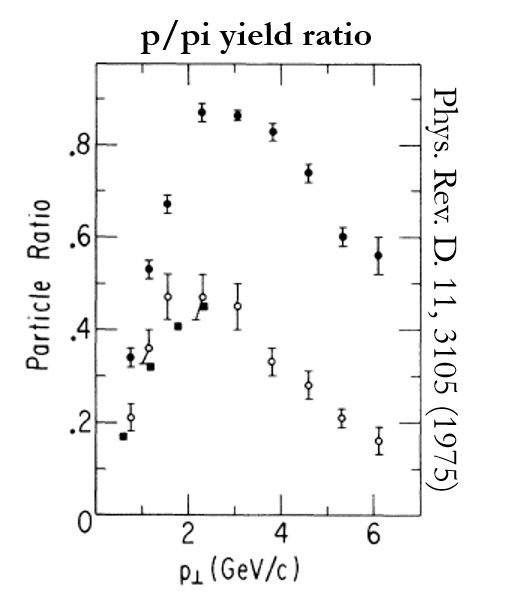
\includegraphics[width=0.5\textwidth]{prevplots/croninratio.JPG}

  \caption[Proton vs pion yield ratio from the Cronin paper]{Proton vs pion yield ratio from the Cronin paper. Closed circles are the ratio obtained by colliding 23.7 GeV protons on tungsten ($A_{eff}= 40.9$). Open circles are the same data scaled to the low limit of single nucleon-nucleon interaction($A=1$).}
  \label{fig:croninratio}    \rule{35em}{0.5pt}
\end{figure}

After the observation of this effect, many set out to come up with theoretical mechanisms that could explain this baryon production preference. These mechanisms can largely be categorized into two types: those where the incoming partons interact with the nuclear medium and those where outgoing partons created after an incoming nucleon hard scatters interacts with the nuclear medium. These two categories are called \textit{Initial State Interactions} and \textit{Final State Interactions.}

\subsection{Initial State Multiple Scattering}
The first attempts at explaining the Cronin Effect were made using initial state interactions. K\"{u}hn in 1975 described a mechanism where incoming partons scatter on nuclear partons, randomizing the direction of the incoming parton before finally colliding with a nuclear quark to produce an event similar to a proton-proton collision\citep{PhysRevD.13.2948} (see fig. \ref{fig:ISIscattering}). Since it is unclear how many ``soft scatters'' happen before the final hard scatter the $p_{T}$ spectrum is broadened which could account for the increase of particle production for the mid $p_{T}$ range. Furthermore, multiple soft scatters are unlikely to produce pions due to the high $p_T$ required to break color confinement, possibly explaining the mid $p_T$ baryon preference.
\begin{figure}[htbp!]
  \centering    \rule{35em}{0.5pt}
    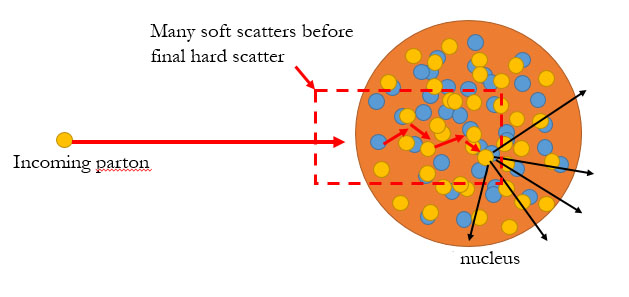
\includegraphics[width=0.8\textwidth]{Figures/ISIscattering.jpg}

  \caption[Illustration of Initial State Multiple Scattering]{Illustration of Initial State Multiple Scattering.}
  \label{fig:ISIscattering}    \rule{35em}{0.5pt}
\end{figure} 

The NA10 collaboration at CERN set out to use back to back lepton probes to study the effect of the nucleus on jets. They collided 140 GeV and 258 GeV negative pions on tungsten targets of various thicknesses and looked for muon pairs produced by quark-antiquark annihilation, also known as a \textit{Drell-Yan Process}.
%\begin{figure}[htbp!]
 % \centering
  %  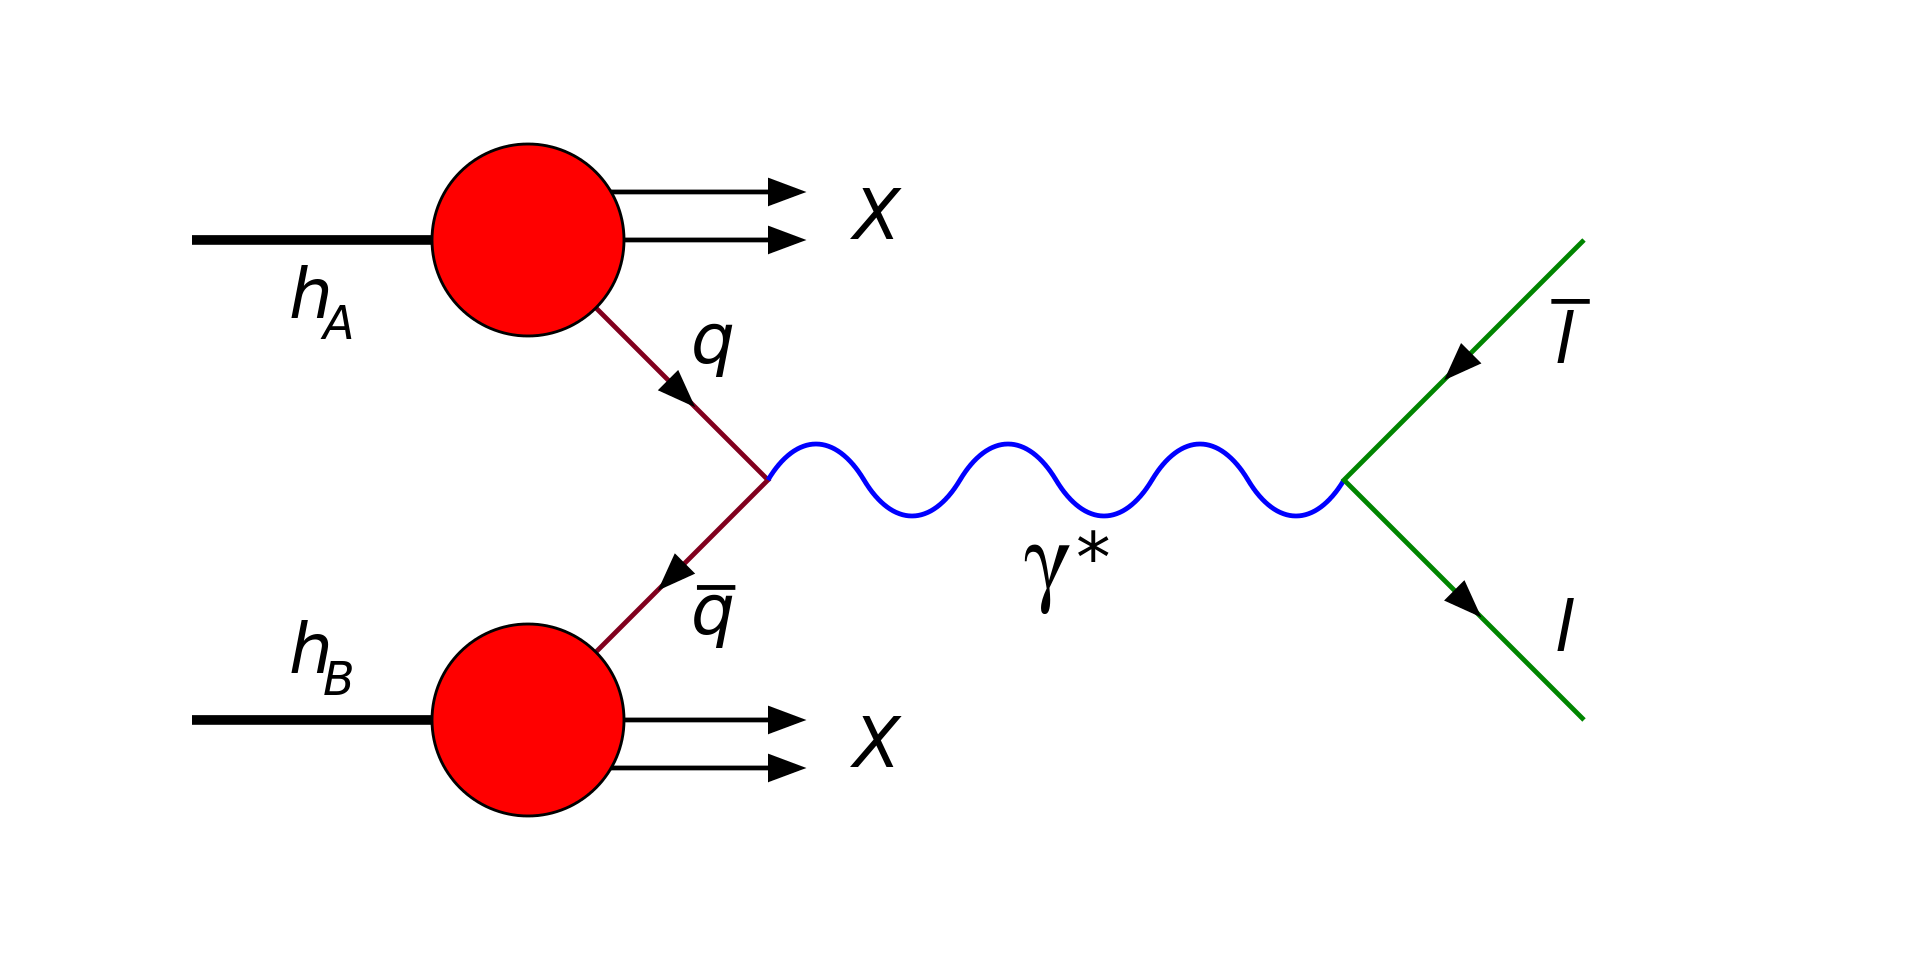
\includegraphics[width=0.7\textwidth]{Figures/DYfeynman.png}
  %  \rule{35em}{0.5pt}
  %\caption[Feynman diagram of Drell-Yan production of dileptons.]{Feynman diagram of Drell-Yan production of dileptons. Quark-Antiquark annihilation produces a lepton-antilepton pair through the exchange of a virtual photon.\citep{PhysRevLett.25.316}}
  %\label{fig:DYfeynman}
%\end{figure}
They found that the mean squared $p_{T}$ of the muon pair did not vary much at all as a function of target thickness which implies that incident partons are not affected by the thickness of the target and therefore that the path length of soft collisions that would broaden the $p_{T}$ spectrum is very short. Furthermore, the E772 collaboration, with an experiment colliding 800 GeV protons on H$_{2}$, C, Ca, Fe, and W targets, showed that Drell-Yan produced dileptons’ mean squared $p_{T}$ did not vary much between the nuclear targets of varying nucleon number\citep{PhysRevLett.66.2285}, i.e. increasing the number of nucleons does not change the net $p_{T}$ much, further showing that initial state contributions to $p_{T}$ broadening are minimal.

\subsection{Final State Multiple Scattering}
\begin{figure}[hbtp!]
\centering    \rule{35em}{0.5pt}
\begin{subfigure}[]{1\textwidth}\captionsetup{width=1.1\linewidth}
    \centering
    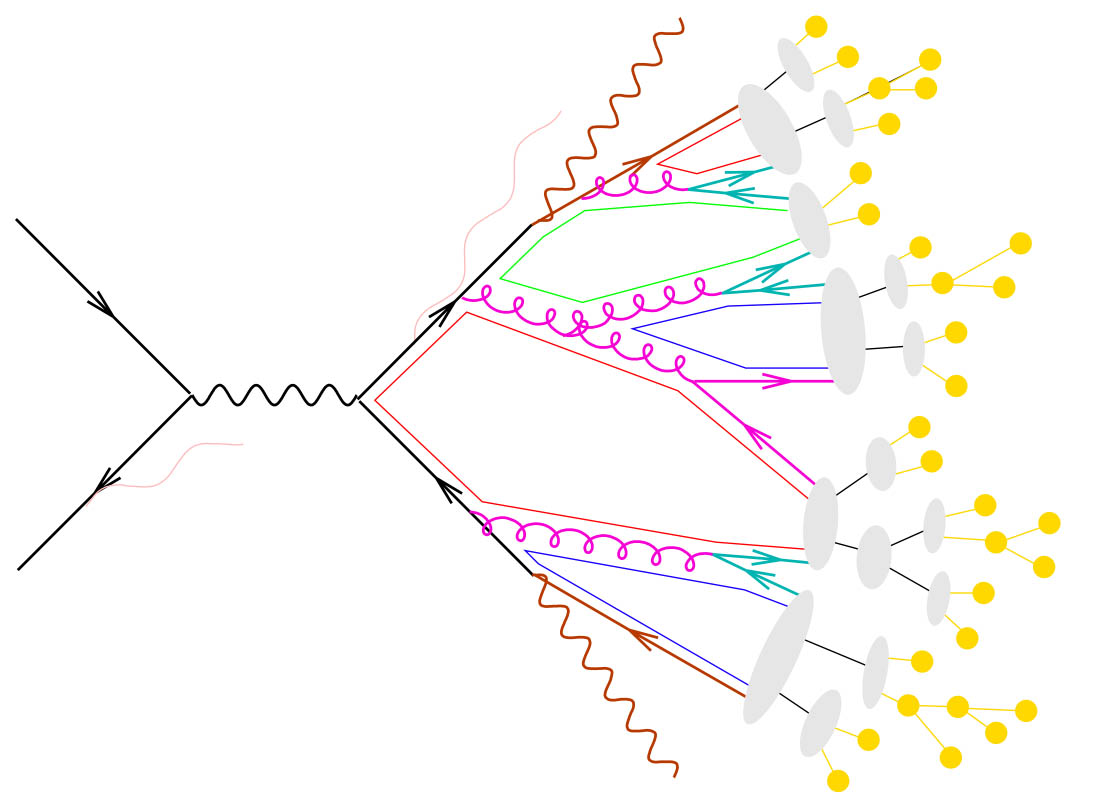
\includegraphics[width=0.5\textwidth]{Figures/jetfeynman.jpg}
\caption{A Feynman diagram\citep{jetfeynmancredit} depicting the annihilation of two quarks creating a force carrying boson which creates a quark-antiquark pair. By the rules of QCD confinement, single particles that have a color charge cannot exist by themselves. As they travel away from the vertex where they were formed they create other colored objects around them in a manner that the net color charge of all particles in the group is colorless. Each group of colorless particles is called a \textit{jet}. Since one jet forming quark is created going one direction, often another is formed going the opposite direction in order to conserve quantum numbers and momentum. This other quark in turn goes on to form its own jet in the same manner. This pair of jets is often referred to as a \textit{dijet}.}
\label{fig:jetfeynman}
\end{subfigure}
\begin{subfigure}[]{1\textwidth}
\captionsetup{width=1.5\linewidth}
    \centering
    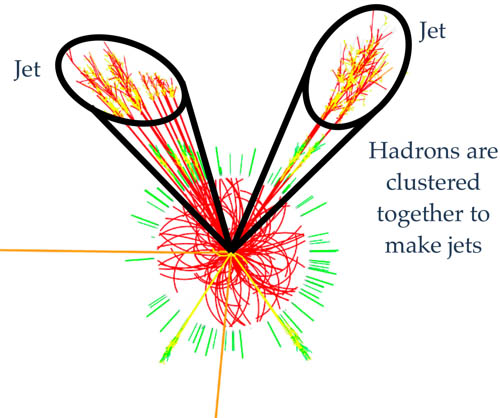
\includegraphics[width=0.5\textwidth]{Figures/jetdiagram.jpg}
\caption{A cartoon illustration\citep{jetdiagramcredit} of how this process might appear in an experiment.}
\label{fig:jetdiagram}
\end{subfigure}
\caption[Feynman and Cartoon diagrams of Jet Formation]{Two illustrations of how jets are formed in particle collisions.}
\label{fig:jetformation}    \rule{35em}{0.5pt}
\end{figure}
In 1991 the E609 collaboration at Fermilab studied phenomena in experiments that collided 400 GeV/c protons with targets made of various nuclear materials including hydrogen and lead\citep{Corcoran:1990vq}. The conditions of interest to them were the creation of two back to back jets produced after an incoming parton hard scattered with a target nucleon, utilizing these dijets as a probe with which to measure the effect of nuclear matter on outgoing partons. They defined a quantity called \textit{planarity} which measured how \textit{back-to-back} two jets are. In their words:
\begin{addmargin}[1.5em]{2em}
``An axis is found which maximizes the sum of the squares of all momentum components ($b_{max}$) along that axis while minimizing the sum of the squares of momentum components perpendicular to that axis ($b_{min}$). Planarity is then defined as: 
\begin{equation}
P = \frac{b_{max}-b_{min}}{b_{max}+b_{min}}.
\end{equation}
For two narrow back-to-back jets, P approaches 1, while for a circularly symmetric event P is 0.''
\end{addmargin}

\begin{figure}[htbp!]
  \centering
    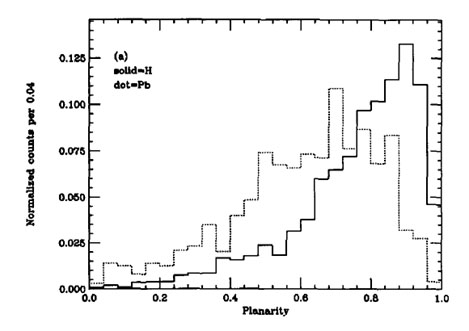
\includegraphics[width=0.8\textwidth]{prevplots/e609planarity.jpg}
    \rule{35em}{0.5pt}
  \caption[Planarity of jets created with protons incident on Pb targets vs H targets.]{Planarity of jets created with protons incident on Pb targets vs H targets.}
  \label{fig:e609planarity}
\end{figure}
Their measurement (fig. \ref{fig:e609planarity}) compared the planarity of dijets created from protons colliding with a hydrogen target with the planarity of those created with collisions on a lead target. They noticed a downward shift in planarity and broadening of the spectrum for Pb dijets compared to H although both had very similar jet widths. This measurement led to a paper in 1993 where they concluded that “Parton hard scatterings within nuclei involve very little nuclear scattering of the incident parton, but that there is substantial nuclear rescattering of outgoing hard scattered partons.\citep{PhysRevLett.70.143}” Because of this, we call this type of mechanism a \textit{Final State Interaction} (for example see fig. \ref{fig:FSIscattering}). While it is true that this could account for the increase in particle production it does not effectively explain why the effect is stronger for baryons than for mesons and why this preference disappears for at high $p_{T}$
\begin{figure}[htbp!]
  \centering
    \rule{35em}{0.5pt}
    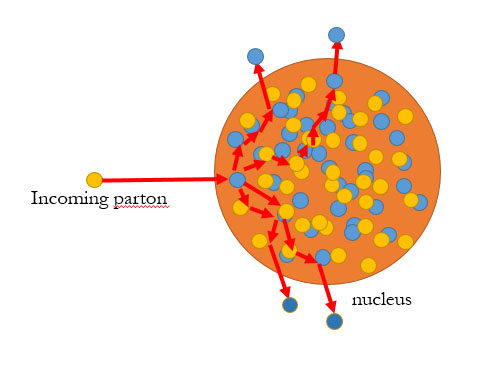
\includegraphics[width=0.7\textwidth]{Figures/FSIscattering.jpg}

  \caption[Illustration of Final State Multiple Scattering]{Illustration of Final State Multiple Scattering.}
  \label{fig:FSIscattering}
    \rule{35em}{0.5pt}
\end{figure} 

\section{Hot Nuclear Matter: Quark Gluon Plasma }
So far this discussion has stayed within the temperature regime where quarks and gluons are confined to hadronic states. As summarized in the previous chapter, physicists had already seen enough hints that new physics was taking place when the energy density reached some critical value and consequently RHIC was commissioned to study this phase change.

\subsection{Collective Flow}
As mentioned, one of the signatures of this phase change was that the medium behaved collectively and that, like a fluid, it flowed. One method of observing this flow is the measurement of the \textit{azimuthal anisotropy} of produced particles. This anisotropy is a measure of how a pressure anisotropy caused by the initial conditions of an ion-ion collision can be correlated to a momentum anisotropy of outgoing particles about the azimuth of the collision. The details of this pressure anisotropy are quantified with a parameter called collision \textit{centrality} which is discussed in detail in section \ref{sect:centrality}, however for this discussion we can think of centrality as how ``head-on'' the collision of two ions is, i.e. do they collide with a large overlap or a small one (see fig. \ref{fig:centvsperiph1}).

\begin{figure}[htbp]
\centering
\rule{35em}{0.5pt}
    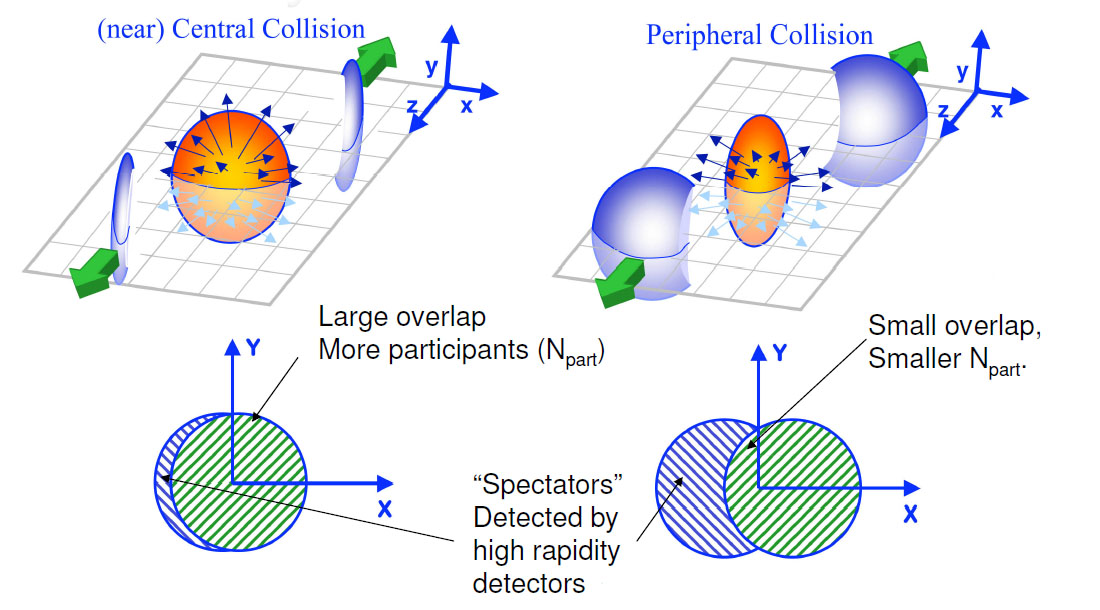
\includegraphics[width=1\textwidth]{Figures/centralvsperipheral.jpg}    

	\caption[Central vs Peripheral collisions, geometry of initial conditions]{An illustration of central vs peripheral heavy ion collisions, geometry of initial conditions. The beam axis goes into and out of the page for the lower diagrams.}
\label{fig:centvsperiph1}
\rule{35em}{0.5pt}
\end{figure}

Therefore it can be seen that peripheral collisions create the largest azimuthal pressure anisotropy and therefore would result in the largest momentum anisotropy of outgoing particles. This pressure anisotropy is largest around the waist of the collision region and weakest at the poles meaning that the collective flow of the QGP would happen with an elliptical shape, also called elliptic flow(fig. \ref{fig:v2auau}), measured by the quantity: $v_2$. There are other types of flow which will be discussed further in chapter \ref{sect:flow}.
    
\begin{figure}[htbp]
\centering 	\rule{35em}{0.5pt}
    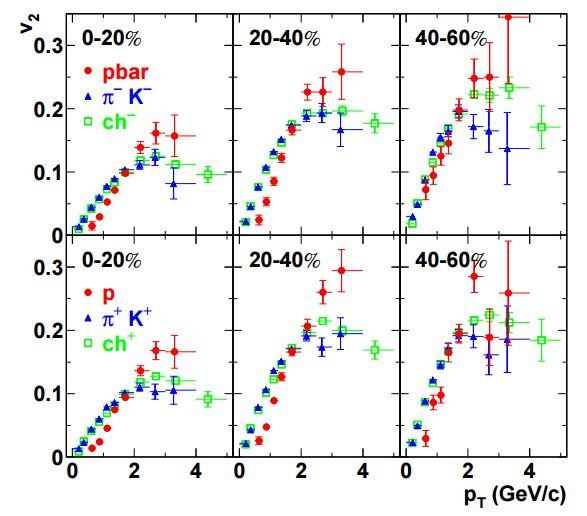
\includegraphics[width=0.5\textwidth]{prevplots/v2auau.jpg}

	\caption[Identified particle elliptic flow vs centrality in 200 GeV Au+Au collisions]{Identified particle elliptic flow vs centrality in 200 GeV Au+Au collisions. Flow is strongest for peripheral collisions due to initial pressure anisotropy indicative of QGP collective behavior. \citep{Adler:2003kt}}
\label{fig:v2auau}	\rule{35em}{0.5pt}
\end{figure}

\subsection{Baryon Enhancement}

\begin{figure}
\centering    \rule{35em}{0.5pt}
\begin{subfigure}[b]{0.7\textwidth}
    \centering
    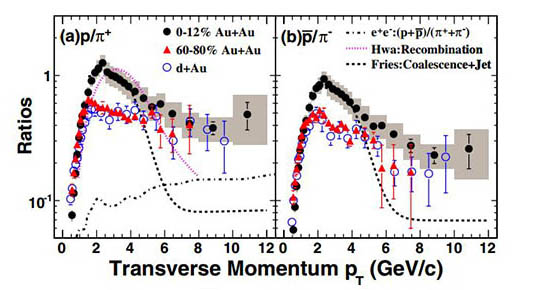
\includegraphics[width=\textwidth]{prevplots/ppiratiocentvsperiph.JPG}
    \caption{ $p/\pi{+}$ and $\bar{p}/\pi^{-}$ ratios for central and peripheral 200 GeV Au+Au collisions. Two leading models are compared to the data as well as the same ratio for 200 GeV d+Au collisions.}
    \label{fig:ppiratiocentvsperiph}
\end{subfigure}
\begin{subfigure}[b]{0.8\textwidth}
    \centering
    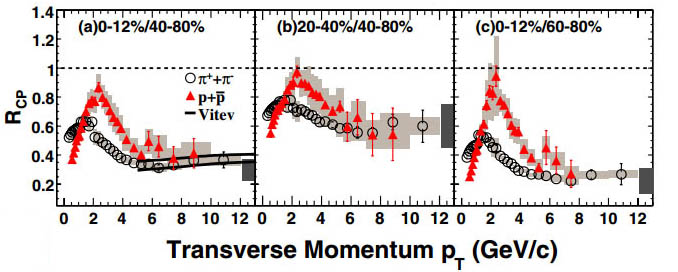
\includegraphics[width=\textwidth]{prevplots/Rcpcentvsperiph.jpg}
    \caption{Nuclear modification factor, $R_{CP}$, comparing nuclear effects on particle production in central versus peripheral Au+Au collisions compared to production in binary scaled p+p collisions (see appendix \ref{nuclmodfactapp} for a summary on nuclear modification factors)}
    \label{fig:Rcpcentvsperiph}
\end{subfigure}
\caption[Evidence of Baryon Enhancement in Au+Au collisions]{$p/\pi$ production ratio and $R_{CP}$ as evidence of Baryon Enhancement in central Au+Au}
\label{fig:baryonenhancementAA}    \rule{35em}{0.5pt}
\end{figure}

Another surprise encountered when studying this new phase of matter was that the production of particles seemed to have a different mechanism compared to p+p collisions. One experimental signature of this was the so called \textit{baryon enhancement} for peripheral Au+Au collisions \citep{PhysRevLett.97.152301}. This result is shown in figure \ref{fig:ppiratiocentvsperiph} which shows the comparative yield between protons and pions in bins of $p_{T}$. The phenomena of interest is the apparent baryon excess in central collision data set for the mid $p_{T}$ range which is strongest at around $p_{T}\approx$ 2 GeV/c and disappears at around $p_{T}\approx$ 4 GeV/c. Similarly, the Nuclear Modification factor for Central and Peripheral collisions also shows this enhancement in the same range (shown in figure \ref{fig:Rcpcentvsperiph}). Though this enhancement is similar to the Cronin effect in cold systems, the Cronin effect had already been attributed to multiple scattering effects of partons on ``frozen'' hadronic states whereas the asymptotic freedom of quarks in the QGP would not cause the same scattering effects since the whole system was outwardly expanding.

\subsection{Theoretical Models of the QGP}
Though many have proposed models to describe this baryon enhancement, I will focus this discussion on a handful of leading models.

\subsubsection{Viscous Hydrodynamics}


\subsubsection{Recombination and Fragmentation}
Following the idea that a phase change in nuclear matter happens when a critical energy density causes deconfinement of quarks and gluons from their bound states as neutrons and protons and that the post-collision evolutionary behavior of this QGP is one that expands rapidly, Rudolph Hwa and C.B. Yang postulated that the enhancement of particle production could be explained by the ways in which the outgoing partons interacted\citep{PhysRevC.70.024905}. They defined two momentum classifications for outgoing partons: those with low transverse momentum (in the hundreds of MeV/c) created by the collective thermal expansion of the QGP which they referred to as \textit{soft} partons, and \textit{hard} partons with high transverse momentum created by hard nuclear scattering processes. Since these hard partons result in jet formation, and jets are comprised of a shower of particles, they use the terminology \textit{shower parton} to describe these hard scatter produced partons. The production of particles could then be described by the way these partons combined combinatorially, i.e. the way thermal partons combined with other thermal partons, the way they combined with hard partons, and the way hard partons combined with other hard partons. This mechanism was termed \textit{recombination} since it relied on the recombining of quarks in partons created from the nuclear collision.

\begin{figure}
\centering    \rule{35em}{0.5pt}
\begin{subfigure}[b]{0.32\textwidth}
    \centering
    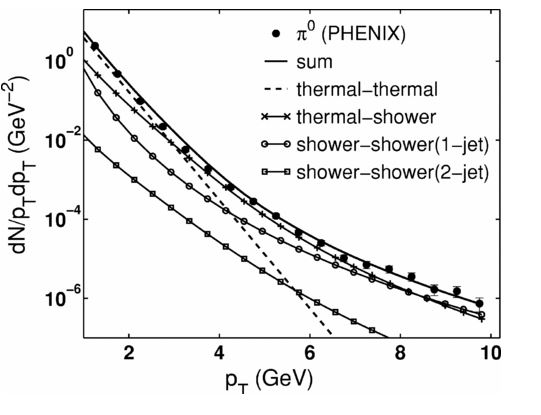
\includegraphics[width=\textwidth]{prevplots/piyieldrecomb.JPG}
    \caption{$p_T$ distribution of pions}
    \label{fig:kyieldrecomb}
\end{subfigure}
\begin{subfigure}[b]{0.32\textwidth}
    \centering
    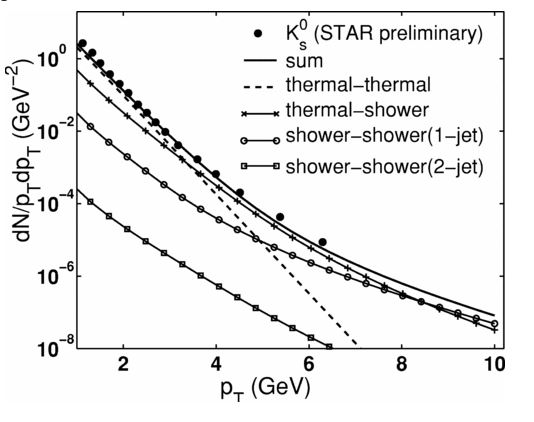
\includegraphics[width=\textwidth]{prevplots/kyieldrecomb.JPG}
    \caption{$p_T$ distribution of kaons}
    \label{fig:kyieldrecomb}
\end{subfigure}
\begin{subfigure}[b]{0.32\textwidth}
    \centering
    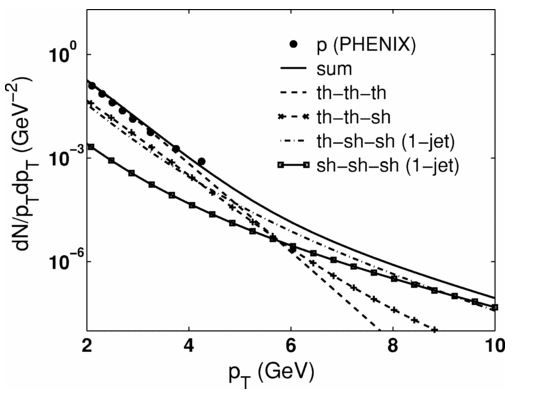
\includegraphics[width=\textwidth]{prevplots/pyieldrecomb.JPG}
    \caption{$p_T$ distribution of protons}
    \label{fig:pyieldrecomb}
\end{subfigure}
\begin{subfigure}[b]{0.5\textwidth}
    \centering
    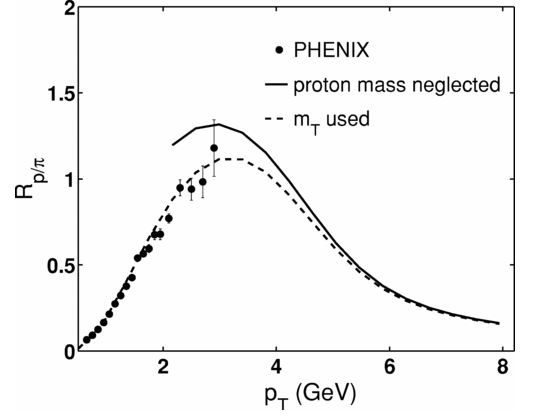
\includegraphics[width=\textwidth]{prevplots/ppiratiorecomb.JPG}
    \caption{$p/\pi$ production ratio versus $p_T$}
    \label{fig:ppiratiorecomb}
\end{subfigure}
\caption[Recombination model compared with Au+Au data]{Au+Au identified particle measurements compared with recombination model predictions. For the $p_T$ distributions we see three distinct regions of recombination, the low $p_T$ range where soft thermal parton recombination dominates, the high $p_T$ range where hard parton recombination dominates, and the middle range where thermal-hard recombination best describes the data.}
\label{fig:hwaAAmodels}    \rule{35em}{0.5pt}
\end{figure}

\begin{figure}[htbp!]
  \centering    \rule{35em}{0.5pt}
    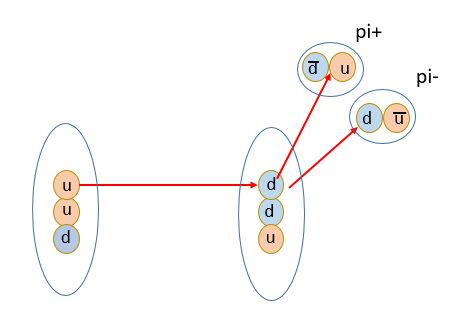
\includegraphics[width=0.5\textwidth]{Figures/fragmentationdiag.JPG}

  \caption[Illustration of an example hard scatter resulting in fragmentation to two pions]{Illustration of an example hard scatter resulting in fragmentation to two pions. Here an up quark scatters with enough energy to scatter and release the down quark from being bound in another nucleon. This occurs with enough energy to create antiparticle partners from the vacuum resulting in the formation of charged pions.}
  \label{fig:fragmentationdiag}    \rule{35em}{0.5pt}
\end{figure} 
Fries, M{\"u}eller, et al. simplified this picture, postulating that the the reason why protons were produced in abundance was simply that following a collision, the building blocks of protons: up and down quarks, are plentiful and that they simply recombine back into their confined states. This mechanism dominates for low $p_{T}$ since outgoing partons are traveling slowly enough that the constituent quarks to remain connected due to color confinement. In contrast to the soft partons, partons created with hard scattering processes are more likely to have enough energy to briefly break color confinement, briefly isolating quarks which then create jets of quark/anti-quark pairs, i.e. mesons. The process of breaking up 3 quark states into quark-antiquark states was then termed \textit{fragmentation}. This two regime model naturally creates a baryon preference for low $p_{T}$ partons that is met with proportional meson production when the parton $p_{T}$ is adequately high enough (see fig. \ref{fig:hwaAAmodels}).

\section{Flow at the LHC}
Up till now it appeared that the lines in the proverbial sand were clear with respect to nuclear matter phase changing and that we had two distinct ways to describe the properties of these two states. On the one side there was cold hadronic matter which had its own experimental signatures that could be observed in the collisions of light ions with heavy ones (such as d+Au). On the other hand, there was hot, deconfined, quark matter which behaved another way and was measured using collisions of two heavy nuclei (as in Au+Au). This notion that the two experimental methods allowed the temperature dependent phenomena to be studied separately was brought into question in 2015 when the \textit{Large Hadron Collider} (LHC) at CERN turned on and entered its second era of measurements. At the Compact Muon Solenoid (CMS) they collected data from p+Pb collisions at 5.02 TeV and compared it to Pb+Pb collisions at 2.76 TeV \citep{Khachatryan:2015waa}. While hydrodynamic phenomena like collective flow was expected in the Pb+Pb data, they did not expect to find flow in systems consisting of a small number of interacting nucleons such as p+Pb(see fig \ref{fig:pPbflow}).

\begin{figure}[htbp!]
  \centering    \rule{35em}{0.5pt}
    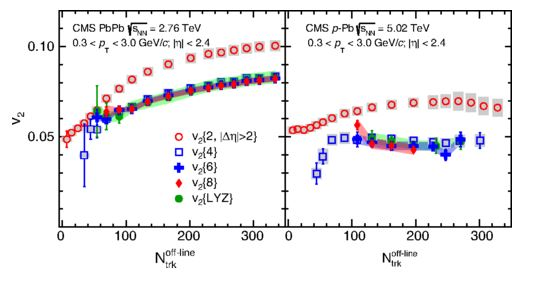
\includegraphics[width=0.7\textwidth]{prevplots/pPbflowLHC.JPG}

  \caption[Elliptic Flow in p+Pb at the LHC]{CMS result from 5.02 TeV p+Pb collisions showing a nonzero elliptic flow signal versus track multiplicity. \citep{Khachatryan:2015waa}}
  \label{fig:pPbflow}    \rule{35em}{0.5pt}
\end{figure} 

The appearance of flow in systems previously thought of as ``cold'' was a sign that perhaps the QGP forms much more easily than was previously expected and that perhaps some phenomena found in cold systems, such as baryon enhancement, could be attributed to mechanisms that found favor in explaining similar phenomena in hot heavy ion systems.

\section{Recombination and Fragmentation for All?}
\label{sect:recombcold}
Furthermore, experimental evidence that the two systems behave quite similarly has been found. In fig. \ref{fig:daaaratios} particle production ratios ($p/\pi$) are compared and we see that the baryon enhancement which was indicative of the QGP formation in peripheral Au+Au collisions is followed extremely closely by data from central d+Au. 

\begin{figure}[htbp!]
  \centering    \rule{35em}{0.5pt}
    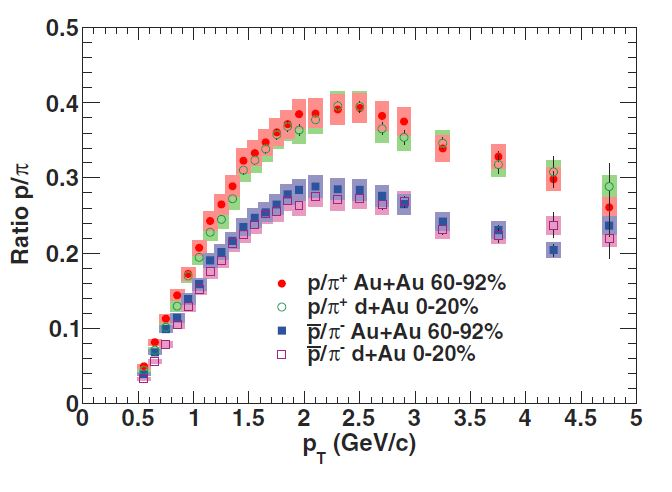
\includegraphics[width=0.7\textwidth]{prevplots/dAvsAAratios.JPG}

  \caption[p/$\pi$ ratios compared for central d+Au and peripheral Au+Au]{p/$\pi$ ratios compared for central d+Au and peripheral Au+Au\citep{PhysRevC.88.024906}}
  \label{fig:daaaratios}    \rule{35em}{0.5pt}
\end{figure} 

The quantity \textit{centrality} will be discussed further in \ref{sect:centrality} but it simply describes how ``head-on'' a collision is. For instance, a collision where two ions collide perfectly head-on is called a \textit{central} collision, whereas if they were just to barely glance each other it would be called a \textit{peripheral} collision. It may seem that the behavior of the two are contradicting since the effect happens in central events for one system and in peripheral events in the other, but we can see from inspection that the two cases are similar. In the Cronin result, a quantity called the number of effective nucleons described the number of nucleons that interacted in a system. If we make the hypothesis that the formation of a QGP is most likely with a higher number of interacting nucleons then it follows that if a QGP were to be formed in d+Au, it would be most likely to form in central collisions. And so, since physicists love reductionism and unification, and that the evidence makes one wonder if a QGP is formed in these simpler systems, it would be advantageous to be able to describe the two systems with a single mechanism.

But are there even the building blocks to support such a notion that QGP is created in such a simple system as d+Au? Recombination is easy to justify in Au+Au since the large number of interacting nucleons makes the formation of the QGP easily achieved and leaves a great abundance of free quarks that are able to recombine. Could there be analogous members at work in the d+Au system? 
\begin{figure}[b!]
  \centering
    \rule{35em}{0.5pt}
    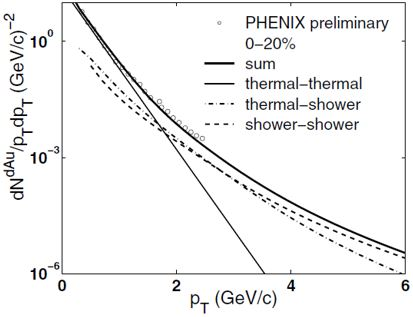
\includegraphics[width=0.5\textwidth]{prevplots/daurecomb.JPG}

  \caption[Pion transverse momentum distribution from d+Au collisions compared to one created with the recombination model]{Pion transverse momentum distribution from d+Au collisions compared to one created with the recombination model}
  \label{fig:daaaratios}
    \rule{35em}{0.5pt}
\end{figure}
Hwa and Yang set out to adapt their recombination model to fit the phenomena in d+Au\citep{PhysRevLett.93.082302}. They asserted that since hard scattering creates jets, as jets traverse the nuclear medium it generates a lot of soft outgoing partons. They argue that these soft partons could behave like an expanding QGP, that is to say, they behave like the thermal partons in Au+Au collisions. Since thermal parton recombination seems to explain baryon enhancement well, and if soft partons behave like thermal partons, could there recombination in d+Au as well? Additionally, if there is, could it be a sign that we should see other signs of QGP formation such as collective flow? 

\section{The Big(ger) Picture}
What other phenomena could hint at the formation of a QGP? Many of the mechanisms discussed thus far pertain to the collective behavior post-thermalization, h

\subsection{Color-Glass Condensate}
A leading model that describes the behavior of nuclei at ultra-relativistic speeds is the \textit{Color-Glass Condensate}. It finds a majority of its support in the results from the H1 and ZEUS experiments at the Hadron Electron Ring Accelerator (HERA) in Germany where the structure of protons was studied by colliding them with electrons at a center of mass energy of 318 GeV\citep{Abramowicz2015}. Their experiments mapped the  \textit{Parton Distribution Function} (PDF) which describes the probability density of particles versus fractional longitudinal momentum. This momentum, the Bjorken \textit{x}, is the fraction of a relativistic hadron's momentum that is carried by a particular parton within it. The PDF from HERA showed that as x decreased, the gluon probability density increased exponentially. At low enough x, the gluon probability dominates the PDF by a factor of 20 (see figure \ref{fig:HERAPDF}). 

\begin{figure}
\centering
\begin{subfigure}[p]{0.8\textwidth}
  \centering
    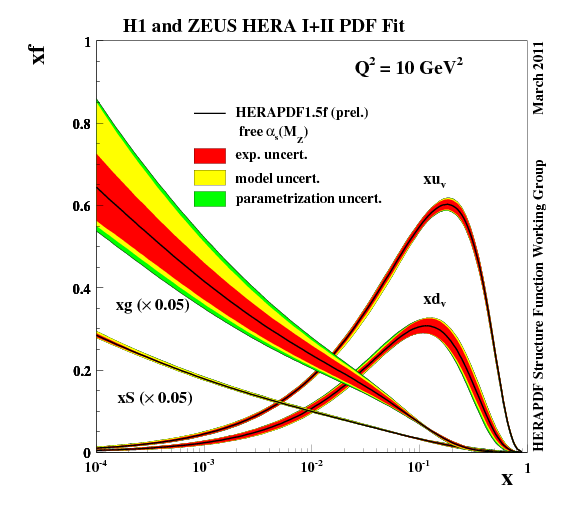
\includegraphics[width=0.8\textwidth]{prevplots/herapdf15f_alpha.png}
  \caption[H1 and ZEUS Parton Distribution Functions]{Combined Parton Distribution Function (PDF) results from HERA experiments\citep{Abramowicz2015} shows probability of finding specific species of particles with fractional momentum, x (Bjorken), inside a proton of squared energy $Q^2 = 10$ GeV$^2$. Carrying the bulk of the momentum are the valence up ($xu_v$) and down ($xu_v$) quarks as expected, however at low x, strange sea quarks (quarks created by quantum fluctuations, $xS$) and gluons ($xg$) dominate. The gluon PDF, specifically, dwarfs the rest by over a factor of 20 at low x.}
  \label{fig:HERAPDF}
\end{subfigure}
    \rule{35em}{0.5pt}
\begin{subfigure}[p]{0.8\textwidth}
  \centering
    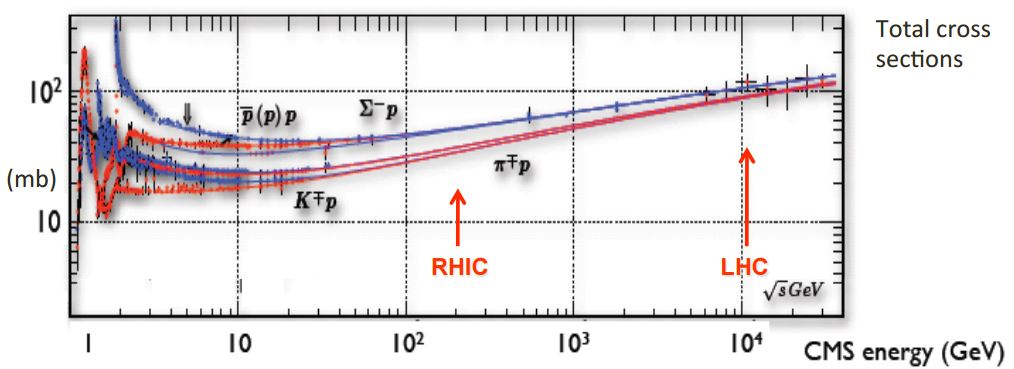
\includegraphics[width=1\textwidth]{prevplots/protoncrosssection.JPG}
  \caption[Proton Cross Section vs Center of Mass Energy.]{Proton Cross Section vs Center of Mass Energy with a variety of probes\citep{PDGcrosssection}. Effective cross section increases with energy implying that there is more inside the proton for incident particles to interact with as the energy of the proton increases.}
  \label{fig:PDGxsection}
\end{subfigure}
\end{figure}

\begin{figure}
\centering
\ContinuedFloat
\begin{subfigure}[h]{0.8\textwidth}
  \centering
    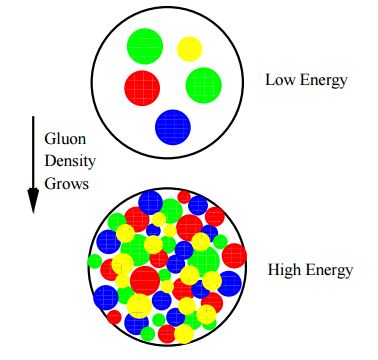
\includegraphics[width=0.5\textwidth]{Figures/gluondensityCGC.jpg}
  \caption[Illustration of gluon saturation in Color-Glass Condensate.]{An illustration of gluon saturation for high energy nucleons\citep{McLerran:2001sr}. As energy increases, the occupation of space by low-x gluons increases.}
  \label{fig:gluonsaturation}
    \rule{35em}{0.5pt}
\end{subfigure}
\caption{}
\end{figure}

Additional support for the model comes from the experimental cross section vs energy. The hadron cross section quantifies the likelihood of a scattering event for an incident beam on a hadron. The classical limit of this cross section is just the cross sectional area of a target but for high energy physics it quantifies the number of interactions that could take place inside of a target (in this case a proton). Figure \ref{fig:PDGxsection} shows that the proton cross section increases above its geometrical cross section ($\pi r_{prot}^2 = $30 mb${^-1}$) to over 100 mb$^{-1}$\citep{PDGcrosssection}. That is, as the energy of a proton increases, it fills with ``something'' that can interact with incident particles. Given the PDF at low-x, it is very highly likely that this ``something'' is an abundance of gluons.

This has interesting implications in the context of Lorentz contracted nucleons. Longitudinally (i.e. along the direction the proton travels), the valence quarks are flattened together due to this contraction, but transversely, the radius of the proton does not change. This leads to a diminishing amount of space inside the proton for the ever increasing number of these low x gluons to occupy. However, from the PDF, we know that the numbers of gluons have to \textit{increase} as we go to lower and lower x, implying that the lower the fractional momentum, the more \textit{saturated} the proton becomes with gluons. This phenomena of large numbers of bosons occupying the same state is where we get the term \textit{condensate} in CGC.

Furthermore, we know that these gluons are force carriers responsible for holding the constituent valence quarks together, however due to the PDF we know that they move orders of magnitude slower than the quarks they are binding together. This inhomogeneity of momentum leads to an inhomogeneity of time scales due to relativistic time dilation. That is, the constituent quarks' relativistic speeds cause the attached slow moving gluons to move incredibly slowly, appearing to be stationary at time scales the high-x quarks experience. This relativistically hindered movement, or textit{frustration}, has drawn analogs to the condensed matter physics term \textit{glass} which is a classification of materials that have the property of behaving like solids on short time scales and flowing like liquids on long ones. 

\subsection{Glasma}
\begin{figure}
\centering
\begin{subfigure}[p]{0.6\textwidth}
  \centering
    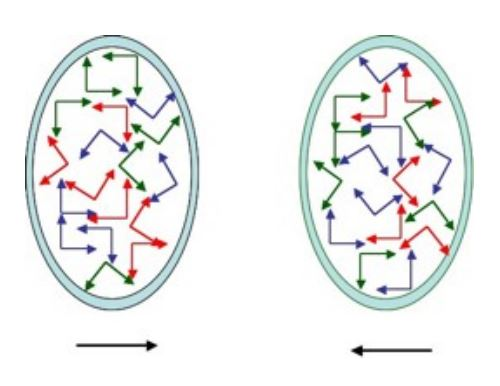
\includegraphics[width=0.8\textwidth]{Figures/collidingCGCsheets.jpg}
  \caption[A cartoon of two color glass sheets just before collision.]{A cartoon of two color glass sheets just before collision. Fields on the sheets exist only in transverse directions.\citep{McLerran:2008es}}
\end{subfigure}
    \rule{35em}{0.5pt}
\begin{subfigure}[p]{0.6\textwidth}
  \centering
    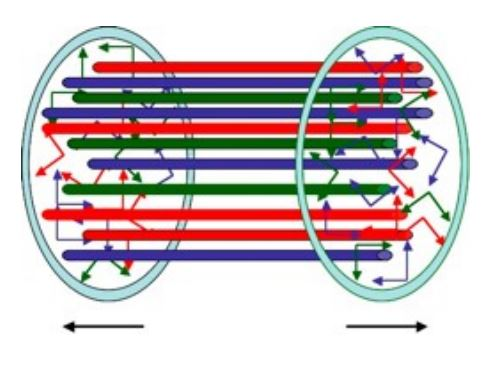
\includegraphics[width=0.8\textwidth]{Figures/glasmatubes.jpg}
  \caption[A cartoon of Glasma formation just after color glass collision.]{A cartoon of Glasma formation. The collision of color glass sheets cause the transverse fields from the two sheets to interact and form longitudinal fields called \textit{color flux tubes} in the moments just after the collision.\citep{McLerran:2008es}}
  
\end{subfigure}
\label{fig:glasmacartoons}
\end{figure}

The CGC has found favor in its ability to describe the initial conditions of the ions before the collision and hydrodynamics describes well the thermalized QGP but the process of thermalization, the equilibration of the quark matter into the QGP, is described by the behavior of the color fields just after the collision.


\subsection{Strangeness Enhancement}
The enhancement of strange particle production has historically been promoted as a sign of QGP formation. As mentioned in section \ref{sect:earlyexperiments}, NA49 and WA97 collaborations were seeing enhancement of kaons compared to pions. 
Note that HERA's PDF shows that not only the number of gluons increase at low-x, but also strange quarks created by quantum fluctuations. A

\section{Moving Forward}
I will show that there is sufficient evidence to say that the nuclear matter created by d+Au behaves collectively and that there should be a non-zero elliptic flow measurement. Furthermore, this elliptic flow is dependent on particle species in that it exhibits baryon enhancement in the mid $p_T$ range indicative of the formation of a QGP. Unknown phenomena of interest is the enhancement of strangeness. Proton and pion flow is an indicator of first generation quark recombination due to the presence of these quarks in atomic nuclei, however strange quarks do not exist in the nucleus and are rather created ``fresh'' from the QGP.  Evidence of strangeness enhancement via kaon flow independent of quark scaling may be further evidence of QGP formation in the previously thought-to-be cold d+Au system. Due to system geometry, flow effects should be maximal with the most central collisions since they create the most interaction of nuclear material (see sect. \ref{sect:recombcold}). Furthermore, as the collisions become more peripheral, the behavior of the system should become more p+p like.
\pagebreak
\pagebreak

% Chapter 3

\chapter{Experimental Apparatus} % Main chapter title
\label{apparatus}
%----------------------------------------------------------------------------------------

\section{The Relativistic Heavy Ion Collider}
\begin{figure}[htbp]
  \centering
    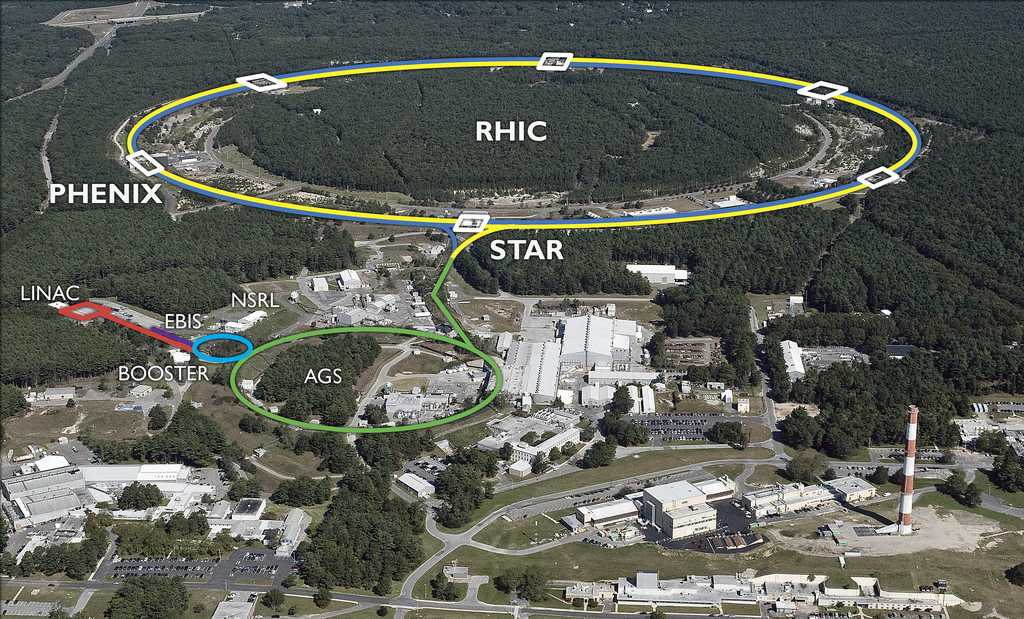
\includegraphics[width=0.6\textwidth]{Figures/RHIC-aerial-HR.jpg}
    \rule{35em}{0.5pt}
  \caption[An Aerial view of BNL]{An Aerial view of BNL with RHIC and the AGS outlined and the locations of PHENIX and STAR mapped}
  \label{fig:Aerial RHIC}
\end{figure}
\indent Based at Brookhaven National Lab (BNL) on the east end of Long Island, New York, the Relativistic Heavy Ion Collider (RHIC) is a particle accelerator and storage ring that is used to study the properties of nuclear matter, specifically the properties, formation of, and phase transition of nuclear matter into a novel state called the Quark Gluon Plasma (QGP).  RHIC accelerates nuclei which are stripped of their electrons (heavy ions) to almost the speed of light and collides them together with enough energy to raise the system's temperature to that which is required to create the QGP. 

\section{From Start to Finish}
\begin{figure}[htbp]
  \centering
    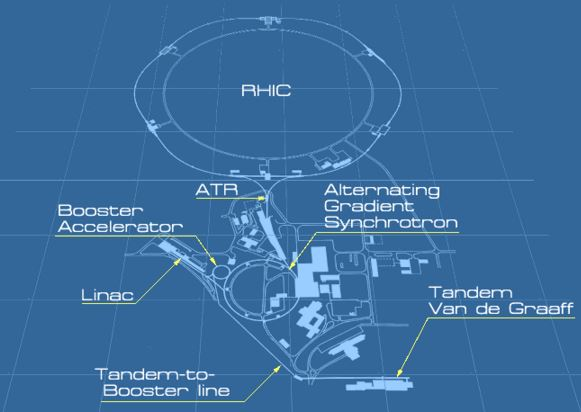
\includegraphics[width=0.8\textwidth]{Figures/RHICdiagram.JPG}
    \rule{35em}{0.5pt}
  \caption[Illustration of all the accelerators used to boost ions to relativistic speeds at RHIC]{Illustration of all the smaller accelerators which are used together in order to boost ions to relativistic speeds at RHIC}
  \label{fig:RHICdiagram}
\end{figure}
The speeds achieved at RHIC is the result of many smaller accelerators working in concert in order to boost the ions' speed faster and faster \citep{RHICaccel}.  Ions begin their journey at a compact source and heavy ion accelerator called the Electron Beam Ion Source (EBIS) (located by the Linear Accelerator (LINAC) in figure \ref{fig:RHICdiagram}). From there they are transferred to the a circular accelerator called the Booster Synchrotron which utilizes long-wavelength radio frequency electromagnetic waves allowing the ions to "surf" on their downward slope. The ions are then fed into the Alternating Gradient Synchrotron (AGS). No slouch in and of itself, the AGS was once the proverbial end-of-the-line where experiments took place and were studied and is responsible for three Nobel Prizes itself: the discovery of the muon neutrino in 1962, the discovery of charge-parity violation in 1963, and the joint discovery of the J/$\Psi$ in 1976. The AGS uses the magnetic field gradients of 240 magnets, alternating them in order to boost the ions to 99.7$\%$ the speed of light after which it is transferred to the AGS-to-RHIC transfer line (AtR). The AtR is like a train switch yard wherein bunches of ions are fed into the RHIC rings. Bunches of ions are sent through either clockwise in one ring or counterclockwise in the other using a switching magnet.

RHIC is comprised of two concentric rings which are 3.8 kilometers in circumference.  These rings use 1,740 helium cooled superconducting magnets to hold beams of these heavy ions which circulate in opposite directions within the two rings.  Along the circumference of RHIC there are six points where the counter-circulating beams can be steered to collide (Interaction Regions or IR). Of these six IR, four have been used to house different detectors: the smaller, now defunct PHOBOS and BRAHMS experiments, and the larger still operational PHENIX and STAR experiments.  

RHIC is an incredibly flexible machine capable of colliding various species of nuclei from protons to Uranium \citep{EBISupgrade} at a wide range of energies.  Heavy ions such as Au can be accelerated as low as 3.85 $GeV/c^{2}$ and as high as 100 $GeV/c^{2}$ \citep{RHIClum} with a combined center of mass energy of 200 $GeV/c^{2}$.  When accelerating protons, RHIC is able to achieve up to 250 $GeV/u$ since the mass/charge ratio is smaller and is able to do so with polarized beams. It is also able to do this asymmetrically, that is to say, with two different species of nuclei, one in each ring.  The system studied in this thesis is one such asymmetric system wherein a deuteron is collided with a gold ion with a center of mass energy of 200 $GeV/c^{2}$ (this system is referred to shorthand as "d+Au").

\section{The PHENIX Detector}

\indent The analysis described in this thesis was made using the PHENIX detector which stands for: \textit{\textbf{P}ioneering \textbf{H}igh \textbf{E}nergy \textbf{N}uclear \textbf{I}nteraction e\textbf{X}periment}. PHENIX is the largest of the experiments at RHIC and was designed specifically to study the QGP using a wide variety of particle probes at a very high rate with high accuracy.  

\begin{figure}[htbp]
  \centering
    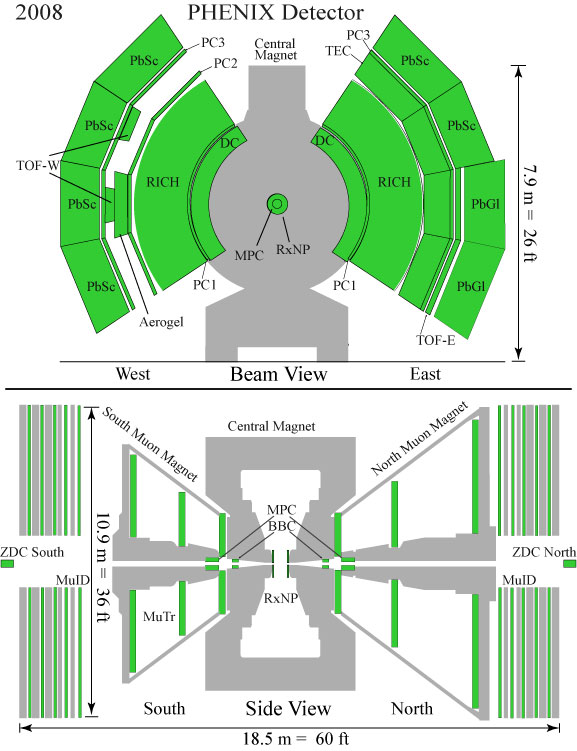
\includegraphics[width=0.8\textwidth]{Figures/Phenix_2008.jpg}
    \rule{35em}{0.5pt}
  \caption[PHENIX Detector Configuration for RHIC Run 8 (2008)]{The configuration of the PHENIX detector for Run 8 (2008)}
  \label{fig:run8config}
\end{figure}
%----------------------------------------------------------------------------------------
It consists of a collection of various detectors assembled into four spectrometers called arms. The muon arms are used for studying physics phenomena at forward rapidity ($\eta$ = $|1.1-2.4|$)\citep{rapidityref} but the system of detectors used for the reconstruction of event tracks of import for this analysis are contained in the \textit{Central Arm}.  

\subsection{Central Arm}
Covering a rapidity range of $\eta$ = $<|0.375|$, the central arm consists of an east and a west arm that cover the azimuth $90^{\circ}$ each \citep{EMCfocus}and is a complex, multi-layered, multi-system spectrometer capable of measuring a variety of particle probes. It is shown on the upper image labeled "Beam View" on figure \ref{fig:run8config} with individual subsystem detectors labeled. No single device is ideal for measuring every aspect of a collision event and as such, particle physicists design these complex detector systems such that different device technologies that are ideal for measuring specific quantities can all be used in concert to gather clean and precise data. Here I will discuss the various individual detectors in the central arm that I use in this analysis.

\subsubsection{Drift and Pad Chambers}
Particle trajectories are tracked using the Drift Chamber (DC) and the Pad Chambers (PC 1,2, and 3). The DC is a multiwire jet-type drift chamber with 12,800 readout channels. It is constructed from 6x80 wire nets in each arm. In principle the DC is similar to a wire chamber; When a charged particle travels through the gas in the DC the gas atoms are ionized and these ions and electrons are accelerated to anode wires which collect this ionization and sends a signal proportional to the ionization effect of the traveling particle. The DC is filled with a gas that is selected to have a uniform drift velocity close to the anode wires, i.e. a gas such that the traveling ions and electrons in the ionized gas have a linear relation in position and time such that $x(t) = v_{drift} * t$ within the active region \citep{DCfocus}, this gas is a mixture of equal parts Argon and Methane also chosen for the mixture's high gas gain amplification and low diffusion coefficient. In doing so and when combined with high accuracy timing caluculation we are able to achieve a more accurate position and trajectory of outgoing particles. The wire nets in the DC are arranged in different predetermined ways with respect to the beam axis. The six nets are designated names: X1, U1, V1, X2, U2, and V2. There are 12 anode wires in each X net and the wires are configured to be parallel to the beam axis so that they can be used to measure the azimuthal angle: $\phi$. The U and V nets are stereo pairs with 4 anode wires in each net and are are oriented such that they are tilted by an angle of 4.5$^\circ$ with respect to the beam axis. This angluar bias allows us to use these nets to measure the track's z-component with high resolution. Furthermore, all wire nets are oriented in layers radially such that outgoing tracks deposit linear, correlatable signals in the DC. Additionally, since the DC is the first detector subsystem that outgoing particles created in a collision pass through, it is also used in conjunction with other detectors in order to accurately determine track trajectory through all of the detectors in the central arm. I will discuss the method of track reconstruction in section \ref{trkrecosect}.

\begin{figure}[htbp]
  \centering
    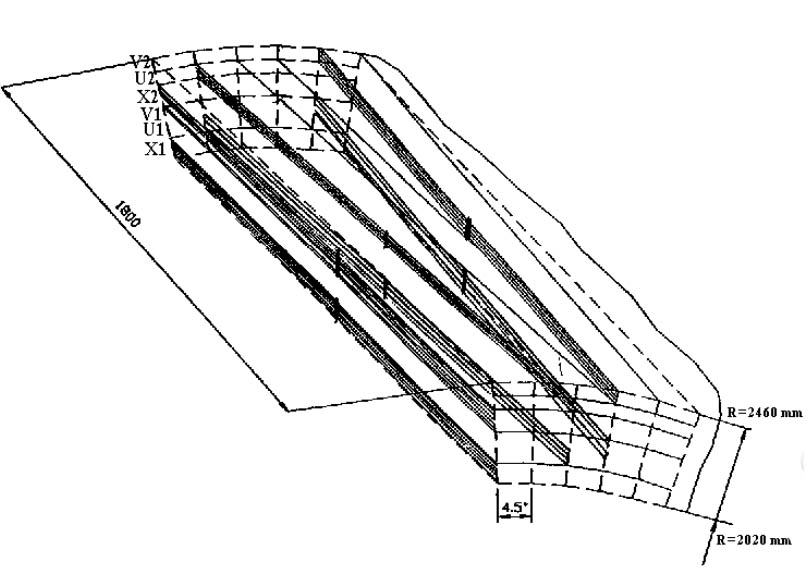
\includegraphics[width=0.6\textwidth]{Figures/dcdiagram.jpg}
    \rule{35em}{0.5pt}
  \caption[Wire net configuration in the DC]{A diagram showing the configuration of the wire nets in the DC}
  \label{fig:dcdiagram}
\end{figure}

The Pad Chambers are three individual layers of pixel detectors. These pixels are arranged in 9 pixel clusters called "pads" that are readout by a single channel \citep{PCfocus}. The pads in the closest-to-collision PC (PC1) are 8.4 mm x 8.45 mm and the pads in PC2 and PC3 are sized to maintain the same angular resolution at farther radial distances. The PC and DC have the same azimuthal coverage as the rest of the central arm and are located at increasing concentric distances from the collision vertex, the DC being the inner most detector, followed immediately by PC1.  PC2 only exists in the west arm however PC3 exists in both arms. The small size of the individual pads allows for a large pixel density important for maintaining the separation of individual track signals in a high luminosity, high multiplicity event such as that of central heavy ion collisions. Since we can use these detectors to accurately determine particle track trajectories, and since charged particles under the influence of a magnetic field curve, the determined curvature can be used to determine track momentum. This track location data is also used to match with other detector data such as calorimetry, time of flight, and Cherenkov counters.
\begin{figure}[htbp]
  \centering
    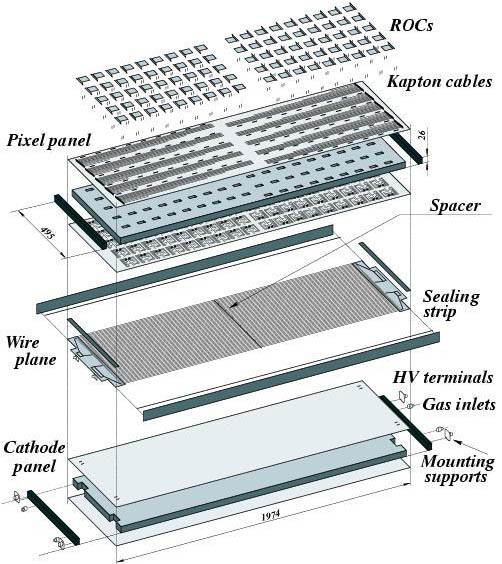
\includegraphics[width=0.6\textwidth]{Figures/pcdiagram.jpg}
    \rule{35em}{0.5pt}
  \caption[Schematic of the Pad Chambers]{A blown up schematic showing the anatomy of the Pad Chambers.}
  \label{fig:pcdiagram}
\end{figure}

\subsubsection{TOF: Time Of Flight Detectors}

In addition to the track matching detectors this analysis utilizes the Time of Flight (TOF) detectors which are high accuracy timing detectors that measure the time it takes for charged particles traveling through the central arm to go from the event vertex to the detector\citep{TOFfocus}. There are two TOF detectors in PHENIX, one on the east DC arm and one on the west arm. Located 5 meters away from the collision vertex and in the lower two sectors of the east arm, the TOF East (TOFE) is a scintillation detector with a timing resolution of $\Delta t_{res} \sim 80 ps$. It covers $\Delta\phi = \pi / 4$ and $\eta < |0.35|$. 

\begin{figure}[htbp]
  \centering
    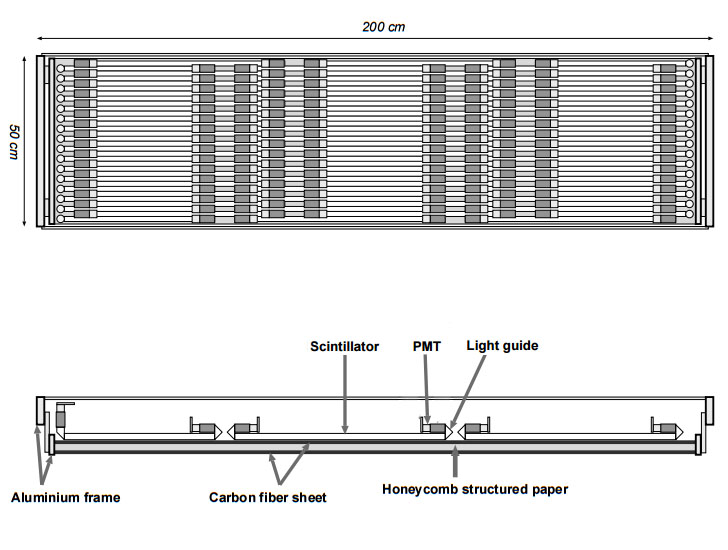
\includegraphics[width=0.8\textwidth]{Figures/TOFEschematic.jpg}
    \rule{35em}{0.5pt}
  \caption[A schematic of the slat layout in the TOFE]{A schematic of the slat layout in the TOFE}
  \label{fig:TOFEschematic}
\end{figure}

Scintillators are a special type of material that fluoresces when it absorbs radiation. The TOFE is comprised of 1000 "slats" of plastic scintillation material with two photomultiplier tubes (PMT) on either end of the slats which amplify the fluorescing photons caused by charged particles that pass through the scintillators. Since we know the length of the slat and the speed of light in the scintillation material we can easily calculate both the time when the particle first hit the slat ($T_{0}$) and the position where the particle hit the slat ($y$).

\begin{equation}
T_{0} = \frac{(T_{1}+T_{2})-L/v}{2} , \, \, y = \frac{T_{1}-T_{2}}{2} v
\end{equation}

Where $T_1$ and $T_{2}$ are the times measured by PMTs 1 and 2 respectively, $L$ is the length of the slat, and $v$ is the speed of light in the scintillator.

\begin{figure}[htbp]
  \centering
    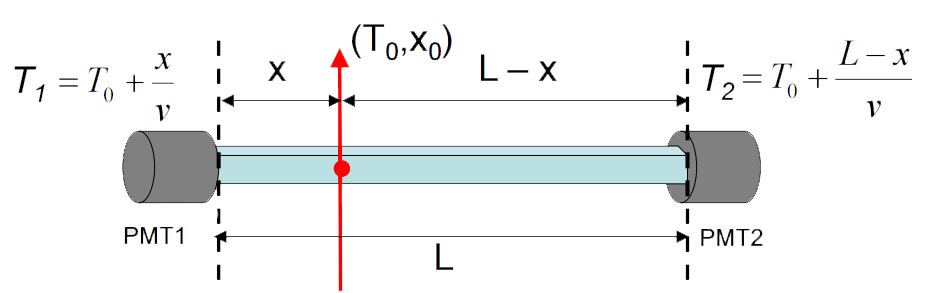
\includegraphics[width=0.8\textwidth]{Figures/TOFEcartoon.jpg}
    \rule{35em}{0.5pt}
  \caption[An illustration of a single slat in the TOFE]{An illustration of a single slat in the TOFE}
  \label{fig:TOFEcartoon}
\end{figure}

In the west arm, the TOF West (TOFW) is a 1024 channel Multi-gap Resistive Plate Chamber (MRPC) detector with a timing resolution of $\Delta t_{res} < 100 ps$, located 4.85 m from the collision vertex and also covering $\Delta\phi = \pi / 4$ and $\eta < |0.35|$. The MRPC works on the same principle as a basic Resistive Plate Chamber which is comprised of two high resistivity plastic (bakelite) plates separated by a volume of gas. On one resistive plate is a sheet of conducting material which is used to maintain a constant electric field across the gas gap. The other resistive plate has an array of conducting readout strips. When a charged particle travels through the gas it causes an electron avalanche similar to what happens in a drift chamber. This electron avalanche is accelerated under the influence of an externally applied electric field toward one of the readout strips resulting in a "hit" signal which is then amplified by electronics. 

\begin{figure}[h]
  \centering
    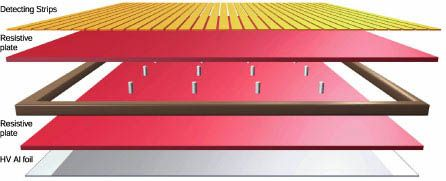
\includegraphics[width=0.8\textwidth]{Figures/RPClayers.jpg}
    \rule{35em}{0.5pt}
  \caption[Diagram of a basic RPC]{Diagram of a basic RPC \citep{CMSRPC}}
  \label{fig:RPCbasic}
\end{figure}

A MRPC is a version of an RPC with alternating layers of the  resistive material and gas gaps sandwiched together with the high voltage surface and readout strips on the outermost sides of the device \citep{Akindinov:2000rq}. The resistive plates inside the sandwich are electrically isolated and are transparent to the fast signals of incoming particles. Initially the externally applied electric field induces charges on the surfaces of the resistive plates causing each of the small gas gaps to be held at the same potential, and since each incoming particle ionizes the gas and deposits the same amount of one charge on one side of the plate and the opposite charge on the other, the potential in each individual gap is held constant. This means that the total signal the strips see is the \textit{sum} of all of the electrical activity in each of small gaps. By using this configuration a greater precision is allowed than conventional RPC designs and lends itself well to high precision timing detectors.

\begin{figure}[ht!]
  \centering
    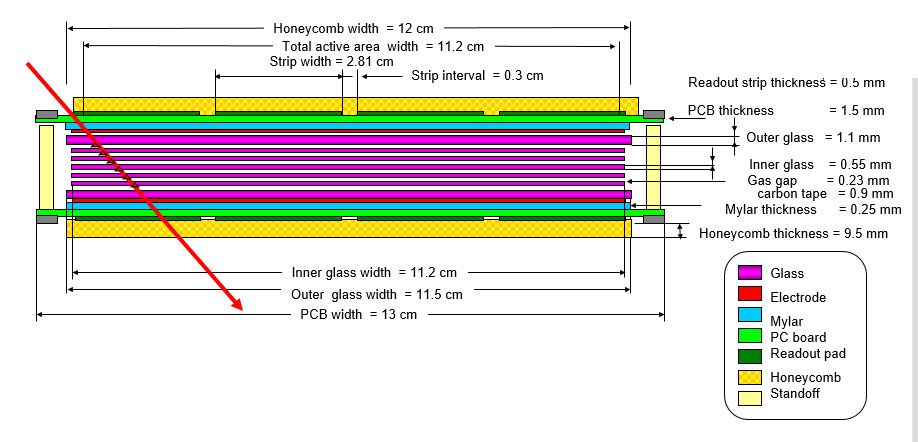
\includegraphics[width=0.8\textwidth]{Figures/MRPC_TOFW.jpg}
    \rule{35em}{0.5pt}
  \caption[Cross sectional diagram of the MRPCs used in the TOFW]{Cross sectional diagram of the MRPCs used in the TOFW}
  \label{fig:MRPCTOFW}
\end{figure}

\subsubsection{ACC: Aerogel Cherenkov Counter}
As track momentum increases the signal width of the particle masses increases. The high resolution capabilities of the TOF detectors only allows them to be able to separate $\pi^{\pm}$, $k^{\pm}$, and $p$ / $\bar{p}$ signals up to certain transverse momentum $p_{T}$ thresholds. The distinct masses of the particles of interest do provide an additional method of separating particle signals since if you were to give two particles of different mass the same momentum they would have distinct velocities. This is the principle with which a Cherenkov detector works. Cherenkov radiation is light that is emitted in a material when a charged particle travels through it with a velocity faster than the speed of light in that medium. This medium, called a Cherenkov radiator, can be carefully selected such that its intrinsic speed of light is such that lighter particles with higher velocities cause Cherenkov radiation but heavier particles which travel slower given the same momentum will not. This threshold is given by:

\begin{equation}
E_{threshold} = \frac{nm}{\sqrt{n^2-1}}
\end{equation}
where n is the index of refraction in the Cherenkov radiator and m is the mass of the particle.
Using this, a Cherenkov detector acts as a logic detector categorizing tracks as those that either "fire" or "veto", that is to say tracks that radiate versus tracks that don't. In the case of separating $\pi^{\pm}$ mesons from $k^{\pm}$ mesons for $p_{T}$ tracks where their mass signals overlap so strongly that they cannot be uncorrelated, the radiator was chosen such that the pions will fire the detector and the kaons will not. Pions and kaons are indistinguishable for $p_{T} > 2.8$ GeV/c, so the radiator chosen to separate the signals is a silica aerogel ($n \approx 1.011$).

\begin{figure}[htbp!]
  \centering
    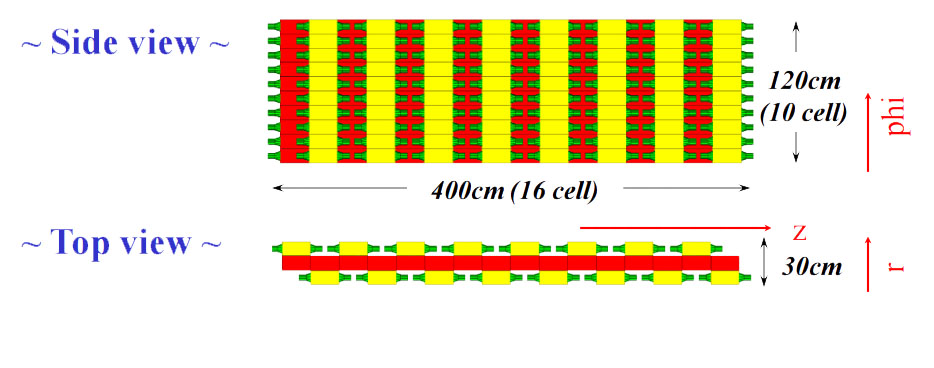
\includegraphics[width=0.8\textwidth]{Figures/ACCschematic.jpg}
    \rule{35em}{0.5pt}
  \caption[A schematic of the Aerogel Cherenkov Counter]{A schematic of the Aerogel Cherenkov Counter}
  \label{fig:ACCschematic}
\end{figure}

The Aerogel Cherenkov Counter (ACC) is comprised of 160 tiles of silica aerogel. Each tile is affixed to an integration cube which allows for radiated cherenkov photons to reflect internally until they hit a PMT. Each integration cube is filled with air and is covered on all exposed sides by a goretex reflector except for the "front" facing aerogel tile side and the two cutouts where the PMTs attach. There are two PMTs located opposite from each other for each cube. To account for the space taken by PMTs on the ends of the tiles the ACC is two sided and the tiles are oriented such that the opposite side tile occupies the gap where PMTs would be situated.  There are 10 rows of 8 tiles on each side for a total of 160 tiles.

\begin{figure}[htbp!]
  \centering
    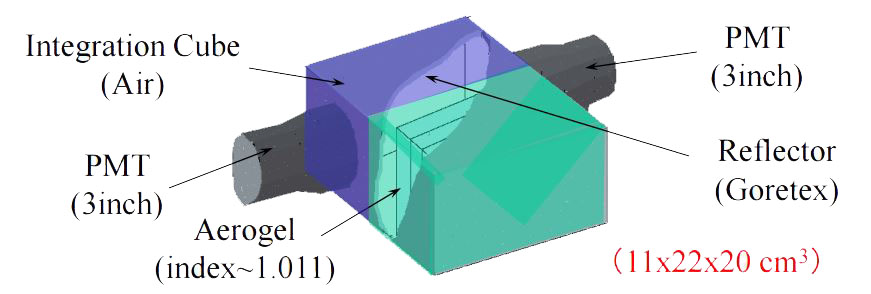
\includegraphics[width=0.8\textwidth]{Figures/aerogelchannel.JPG}
    \rule{35em}{0.5pt}
  \caption[A schematic of one tile in the ACC]{A schematic of one tile in the ACC}
  \label{fig:accchannel}
\end{figure}

The ACC is located in the west arm covering the half of the azimuthal coverage that the TOFW covers and with the same rapidity coverage. When used in conjunction with the TOFW it can provide pion/kaon separation for $p_{T} < 4$ GeV/c and can discriminate protons for $p_{T} < 7$ GeV/c.  The total capabilities of the combination of the TOFW + ACC is shown in the following chart.

\begin{figure}[h!]
  \centering
    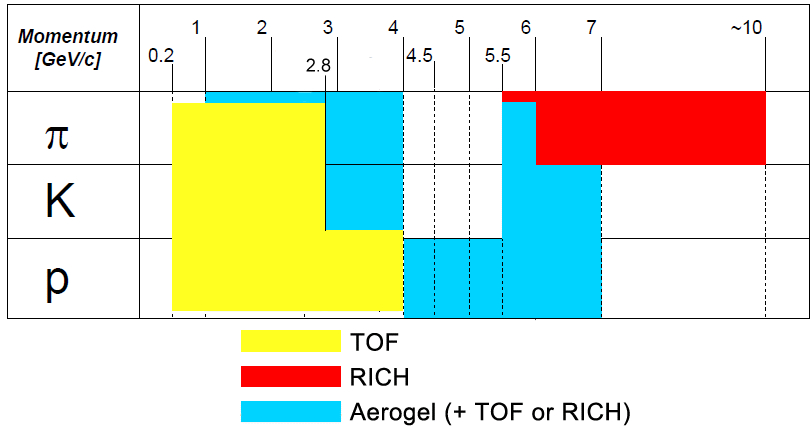
\includegraphics[width=0.8\textwidth]{Figures/accrange.jpg}
    \rule{35em}{0.5pt}
  \caption[Chart of Particle Identification capabilities over a range of transverse momentum]{Chart of Particle Identification capabilities over a range of transverse momentum}
  \label{fig:PIDrange}
\end{figure}

\subsubsection{EMCal and RICH: Electromagnetic Calorimeter and Ring Imaging Cherenkov Counter}
Two other detectors that provide important track data are the \textit{Electromagnetic Calorimeter} (EMCal) and the \textit{Ring Imaging Cherenkov Counter} (RICH). Each arm has full coverage with both the RICH and the EMCal and they are often used together in order to study electrons via the EMCal/RICH Trigger (ERT).

As evident from it's name, the RICH is a Cherenkov counter that is used in a similar fashion as the ACC: to discriminate between particle species using Cherekov radiation as a logic trigger. In the case of RICH, we are interested in separating pion and electron signals. It is filled with CO$_2$ which was chosen because it would allow electrons to radiate at very low $p_T$ ($>$ 0.018 GeV/c) while pions will not until the relatively high $p_T$ of 4.87 GeV/c. Cherenkov radiated photons are emmitted parallel to each other along the track path as electrons move through the detector. The outer surface of the RICH is a series of mirrors arranged to form a spherical mirror which focusses that Cherenkov light onto the 2560 PMTs/arm which line the inner surface of the RICH. This results in a ring shaped Cherenkov signature as measured by the PMTs, hence the name: Ring Imaging Cherenkov Counter. 

\begin{figure}[h!]
  \centering
    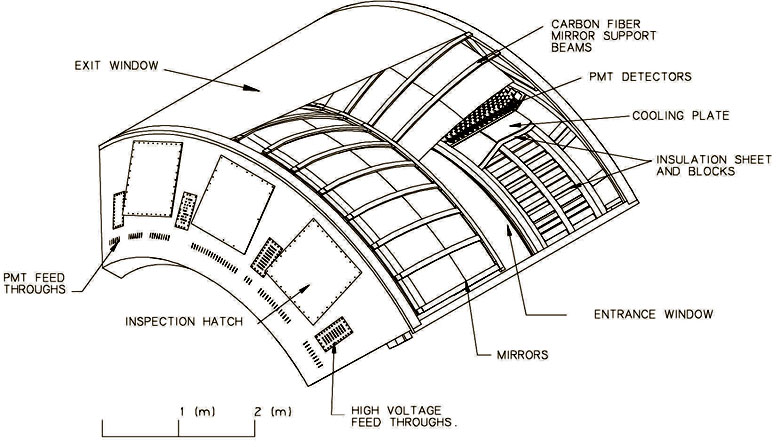
\includegraphics[width=0.8\textwidth]{Figures/RICHdiagram.jpg}
    \rule{35em}{0.5pt}
  \caption[A diagram of the RICH]{A diagram of the RICH}
  \label{fig:RICHdiagram}
\end{figure}

\begin{figure}
\centering
\begin{subfigure}[p]{0.5\textwidth}
    \centering
    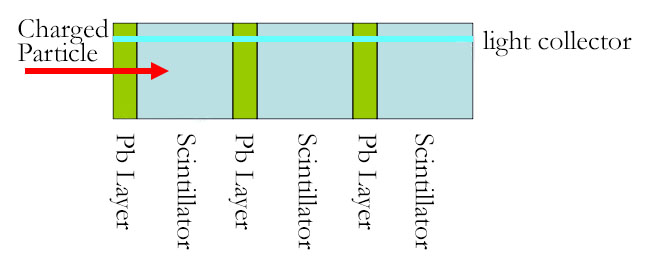
\includegraphics[width=\textwidth]{Figures/PbScschematic.jpg}\ssp
    \caption{Schematic of a PbSc module. Pb layers cause EM showers which create light in the scintillators and are detected by the light collectors.}
    \label{fig:pbscmodule}
\end{subfigure}
\begin{subfigure}[b]{0.6\textwidth}
    \centering
    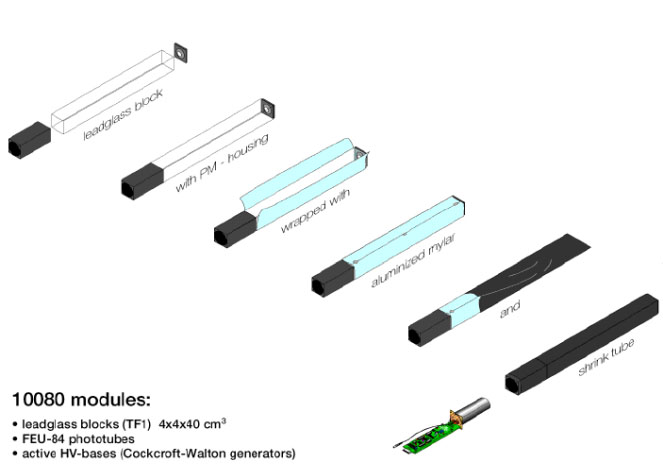
\includegraphics[width=\textwidth]{Figures/PbGlmodules.jpg}
    \caption{Construction of PbGl modules.}
    \label{fig:ppiratiocentvsperiph}
\end{subfigure}
\begin{subfigure}[b]{0.6\textwidth}
    \centering
    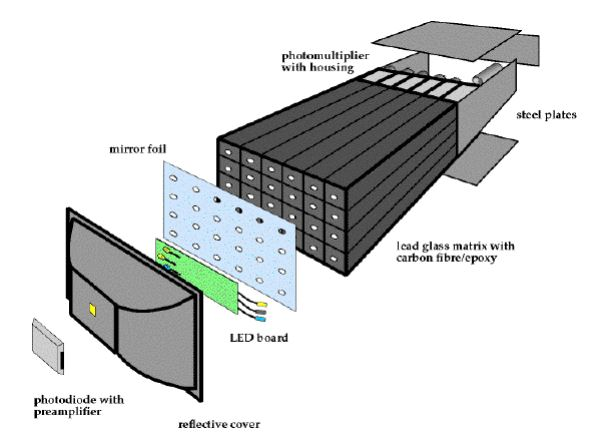
\includegraphics[width=\textwidth]{Figures/pbglsupermodule.JPG}
    \caption{One PbGl super module}
    \label{fig:Rcpcentvsperiph}
\end{subfigure}
\caption[Schematics of EMCal components]{Schematics of EMCal components}
\label{fig:baryonenhancementAA}
\end{figure}
\dsp

The EMCal provides an energy measurement for charged tracks and is broken up into eight sectors, four sectors in each arm \citep{EMCfocus}. Six of the sectors (all four of the west arm and the top two in the east arm) are made of channels comprised of alternating layers of lead and scintillator (PbSc) material. The lead layers cause incoming particles to shower into the scintillator layers which generate light that is detected by PMTs. The lower two sectors in the east arm are comprised of 10,080 uniform lead glass Cherenkov radiator towers (PbGl). These towers have PMTs attached on one end and are wrapped individually in reflective mylar and shrink wrapped to form \textit{modules}. They are then placed in grid-like networks and each 16 module x 12 module structure is read out by one photodiode/preamplifier combination. 

Though it may seem odd to have two types of detectors in the EMCal, there is a method to the madness. Both have their own strengths, PbSc is more linear in response and is better at timing than PbGl thanks to its alternating layers, whereas PbGl is a tried and true design used in previous experiments such as WA98 at the SPS at CERN for it's exceptional granularity and accurate energy measurement. Because they are two separate systems, they have different systematics and therefore we have a higher confidence level for the physics results from the EMCal. 

As mentioned, the EMCal and RICH are used together to form a level 1 trigger to classify charged tracks. Since the RICH is tuned to radiate with electron tracks and the EMCal measures all charged tracks, we know that tracks that result in signals in both the EMCal and the RICH are most likely electrons, whereas tracks that only have signals in the EMCal are likely charged hadrons.

\begin{figure}[h!]
  \centering
    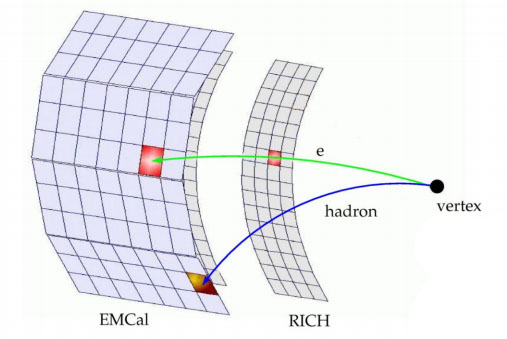
\includegraphics[width=0.5\textwidth]{Figures/ERT.jpg}
    \rule{35em}{0.5pt}
  \caption[A drawing of example ERT events]{A drawing of example ERT events}
  \label{fig:ERT}
\end{figure}

\subsection{Forward and Global Detectors}
Though the bulk of this analysis is dependent on the central arm detectors, many aspects of reconstruction, namely event characterization (start of the event timer, the event vertex, centrality, and event reaction plane) is dependent on a handful of forward detectors which I will briefly discuss here.

\subsubsection{BBC: Beam-Beam Counter}
Of the forward detectors, the \textit{Beam-Beam Counter} (BBC) is probably the most important because of its ability to measure the various global event parameters. There are two BBCs, one on the north side and one on the south side of PHENIX both equidistant from the center of the interaction region (IR). The constituent detector elements are made of quartz Cherenkov radiators attached to meshed dynode PMTs housed in hexagonal encasement. These elements are arranged in a toroidal shape in order to allow the ion beams to pass through the center while still getting full $2\pi$ azimuthal coverage. The BBCs cover 3.1$\leq \Delta \eta \leq<$4 in pseudorapidity.
\begin{figure}
\centering
\begin{subfigure}[b]{0.4\textwidth}
    \centering
    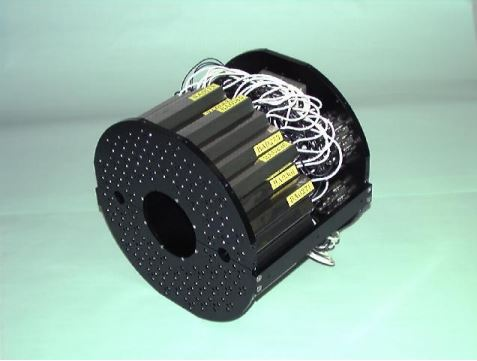
\includegraphics[width=\textwidth]{Figures/bbcrender.JPG}
    \caption{An illustration of a BBC}
    \label{fig:ppiratiocentvsperiph}
\end{subfigure}
\begin{subfigure}[b]{0.4\textwidth}
    \centering
    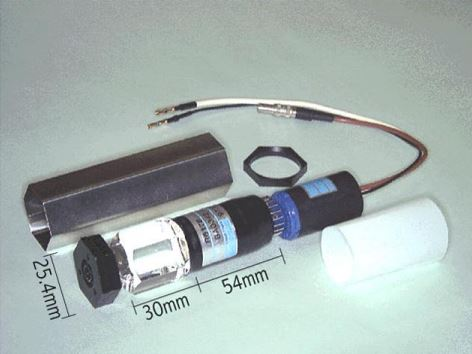
\includegraphics[width=\textwidth]{Figures/bbcsinglechannel.JPG}
    \caption{A single element of the BBC}
    \label{fig:Rcpcentvsperiph}
\end{subfigure}
\caption[The Beam Beam Counter]{The Beam Beam Counter}
\label{fig:baryonenhancementAA}
\end{figure}

\subsubsection{ZDC/SMD: Zero Degree Calorimeter and Shower Max Detectors}

\begin{figure}[h!]
  \centering
    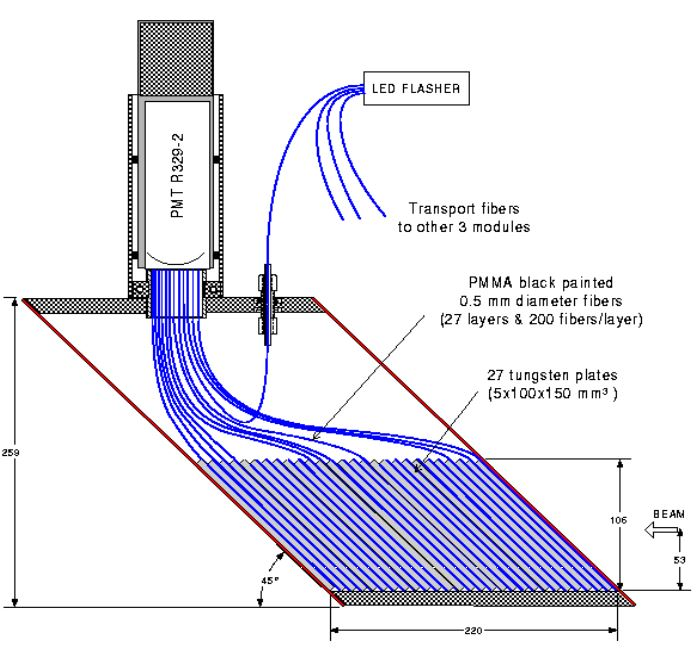
\includegraphics[width=0.7\textwidth]{Figures/ZDCschematic.JPG}
    \rule{35em}{0.7pt}
  \caption[Schematic showing the layout of fiber optics in the ZDC]{Schematic showing the layout of fiber optics in the ZDC}
  \label{fig:zdcvsbbc}
\end{figure}

Crucial to the determination of event centrality is the ability to count the number of spectator particles. Since neutrons are have no charge we can place a calorimeter at high rapidity behind an IR dipole magnet which we can use to "sweep" away charged particles like proton spectators and other charged track noise. The \textit{Zero Degree Calorimeter}\citep{ZDCfocus} is comprised of a ribbon of acrylic fiber optic strands sandwiched between two tungsten plates. The tungsten plates act as a dense absorber for the neutrons to hit and shower into resulting in detectable photon yield in the fiber optic ribbon. Sandwiched between modules of the ZDC is a hodoscope called the \textit{Shower Max Detector} (SMD). The SMD is comprised of 21 0.5 cm x 0.5 cm scintillators and is used to measure the centroid of the shower in cartesian coordinates since the ZDC only measures energy\citep{phenixzdc}. The ZDC is used in conjunction with the BBC in order to determine centrality. Since more peripheral collisions mean more spectators and therefore more neutrons to hit the ZDC, the higher the energy measured by the ZDC the more peripheral the event (see fig \ref{fig:zdcvsbbc}\citep{Ghosh2001}).

\begin{figure}[h!]
  \centering
    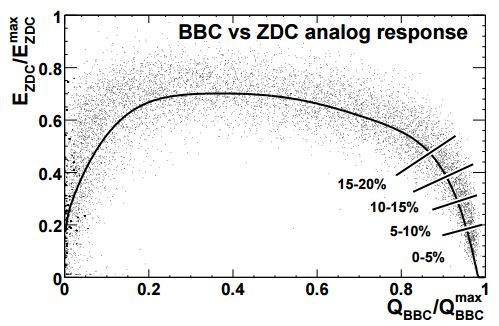
\includegraphics[width=0.5\textwidth]{prevplots/bbczdcanaresponse.JPG}
    \rule{35em}{0.5pt}
  \caption[Centrality bins as determined by ZDC energy versus BBC charge sum]{Centrality bins as determined by ZDC energy versus BBC charge sum\citep{Ghosh2001}}
  \label{fig:zdcvsbbc}
\end{figure}

\subsubsection{MPC: Muon Piston Calorimeter}
The \textit{Muon Piston Calorimeter} (MPC) was a needed upgrade to PHENIX that provided calorimetry at very high rapidity\citep{kleinjanthesis}. It was installed in two parts: first in the south in 2005, then in the north in 2006 and was commisioned to reconstruct $\pi^{0}$ and $\eta$ mesons for various forward physics analyses. Nestled in a gap in the piston of the Muon Magnet Arms, it provides full azimuthal coverage at $3.1 \leq  | \eta | \leq 3.7$ ($3.9$ in the north) and is comprised of 196 (220 in the north) Lead Tungstate $PbWO_4$ crystal scintillator towers attached to avalanche photodiodes with preamplifiers to measure the electromagnetic shower photons. For this analysis, the MPC is used as a another measurement point for determining the reaction plane resolution correction. 

\begin{figure}[h!]
  \centering
    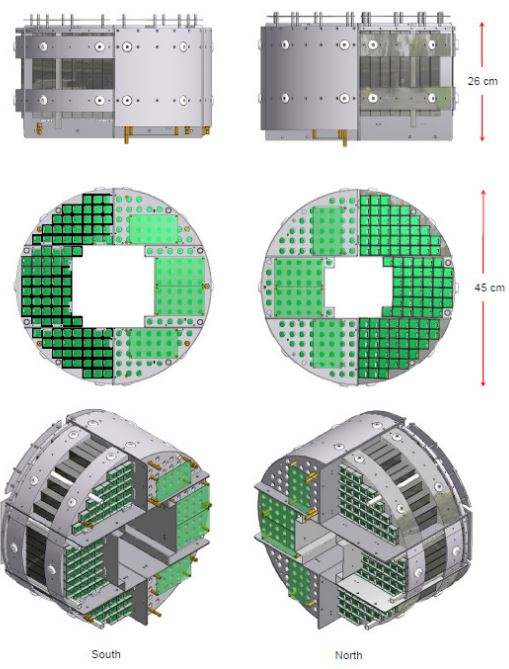
\includegraphics[width=0.7\textwidth]{Figures/mpcschematic.JPG}
    \rule{35em}{0.5pt}
  \caption[Schematic of the MPC]{Schematic of the MPC}
  \label{fig:mpcschematic}
\end{figure}

\subsubsection{RXNP: Reaction Plane Detector}
Of particular interest for this analysis is the determination of the reaction plane. This will be discussed in further detail in a later chapter but I will cover the basics of the technical specifications here. The \textit{Reaction Plane Detector} (RXNP) is a forward detector subsystem \citep{RXNPfocus} with full azimuthal coverage in 12 segments. It has two segments in rapidity: an inner segment that covers $1.5 \leq \eta \leq 2.8$ and an outer segment that covers $1.0 \leq \eta \leq 1.5$. There are two RXNP detectors, one on each muon arm and all the segments are made of 2 cm thick plastic scintillators with a 2 cm layer of lead placed directly in front that acts as a converter causing all tracks to shower before hitting the scintillators \citep{RXNPfocusER}.  

\begin{figure}[h!]
  \centering
    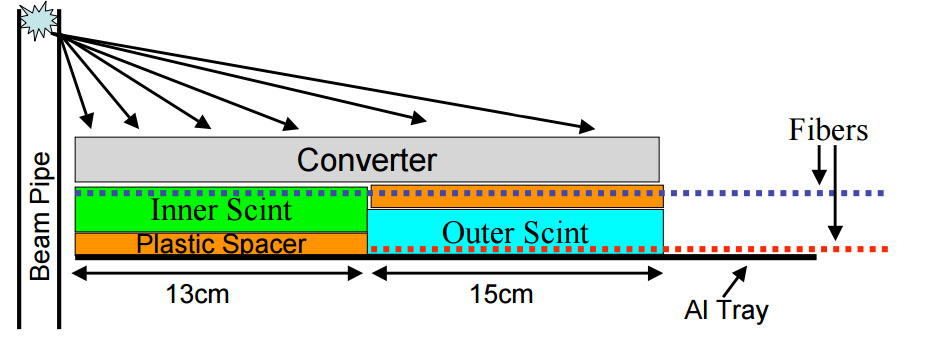
\includegraphics[width=0.7\textwidth]{Figures/RXNPschem.jpg}
    \rule{35em}{0.5pt}
  \caption[Cross sectional diagram of RXNP layers]{Cross sectional diagram of RXNP layers}
  \label{fig:RXNP}
\end{figure}

\section{The DAQ}
Each of these detector subsystems captures large amounts of data per event, and with the high luminosity of RHIC collisions in the millions of events per second, the events don't stop and wait for our computation systems, reconstruction, or network storage capabilities to catch up. The process of optimizing data collection created from a high-event-rate, high track multiplicity experiment, in the form of dozens and dozens of event and track variables collected by thousands of individual readout channels in a handful of individual subsystems, all funneled through a single data acquisition system that organizes everything and prepares the data for analysis is an intricate and chaotic symphony \citep{DAQfocus}. In order to do this, the DAQ breaks up the dataflow into smaller groups called \textit{partitions} which are assembled from the smallest collection of data channels that can collect coherent data which we call \textit{granules}. This partition model with granules allows PHENIX to collect even if some subsystems are down for whatever reason, an ability of great importance since funding for RHIC runs only allows us to have collisions for a few months a year, meaning that during data taking runs it is of utmost importance that we collect as much data as possible, stopping only to maintain the machinery. In practice this results in three 8 hour manned shifts a day, 7 days a week, for the duration of the run, where data taking only stops to re-inject RHIC with ions or on machine-wide agreed upon "access days" where all collaborations and the Collider-Accelerator Department agree to do their maintenance and repair work with no beam in RHIC.

Each granule consists of a Granule Timing Module (GTM), a Front End Module (FEM), and a Data Collection Module (DCM).  The GTM synchronizes with the overall DAQ clock which is also synchronized with the RHIC clocks. These clocks optimize the amount of time the DAQ is actively processing data (called its \textit{livetime}) so that the DAQ is live when bunches of ions are colliding at a maximum rate. The FEMs take the raw output from the preamplifiers in the individual readout channels of a detector subsystem and organizes them into coherent data packets which are transferred over fiber optics to the DCMs which act as a sort of stop light regulating the flow of data into buffers with the GTM clock so that data packets from various subsystems are in sync with each other from the same event as they go into the buffer boxes before being transferred to storage. Even with this timing and granule optimization, RHIC's event rate is so high that it is impossible to collect every track that passes through its subsystems. The means of making sure the only events we capture are events that contain rare processes is called \textit{triggering}. There are many triggers at different levels of the DAQ, for example the aforementioned ERT is a trigger that allows us to only collect data on electron events, events that are of interest for dilepton analyses such as Drell-Yan and J/Psi measurements. The master trigger that sets the timing for the whole DAQ is called the Global Level 1 trigger or the GL1. It synchronizes large track multiplicity signal coincidence collected by the ZDC to the start of the event and checks to see if the buffers in each granule are clear. Other triggers such as \textit{Local Level 1} (LL1) utilize data from the BBCs to ensure the event vertex happens within a region that will result in acceptable track acceptance.

\begin{figure}[h!]
  \centering
    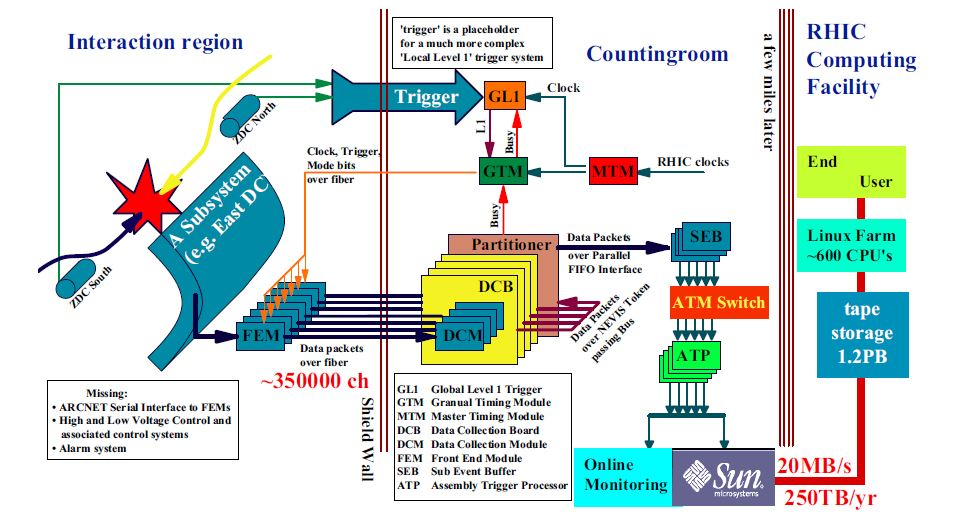
\includegraphics[width=1\textwidth]{Figures/DAQ.jpg}
    \rule{35em}{0.5pt}
  \caption[A diagram of the data flow of PHENIX data through the DAQ]{A diagram of the data flow of PHENIX data through the DAQ}
  \label{fig:DAQ}
\end{figure}

\pagebreak
\pagebreak

\chapter{Heavy Ion Collisions: A Primer} % Main chapter title
\label{hicollisions}
%----------------------------------------------------------------------------------------
\section{Measurable Quantities}
Due to the complexity inherent in colliding large nuclei containing a large number of nucleons (for instance 197 nucleons in Au) there is a multitude of metrics we can use to quantify the collision and the evolution of what happens after. For clarification, when talking about high energy physics analyses we refer to all data gathered from a single collision of two nucleons as an \textit{event}. The location where the collision takes place is called the \textit{event vertex} or often in collaboration literature since the z-axis is along the beam axis, the \textit{z vertex}. The high luminosity of heavy ion collisions (437 $nb^{-1}$ in 9 weeks for the data used in this analysis: Run 8 d+Au), produces a plethora of events (10.6 billion events). As these particles travel from the event vertex through the various layers of detectors under the influence of the PHENIX magnetic field it leaves its own signature on each detector it passes through. These signatures for each given particle can be matched to form a trajectory from the event vertex through PHENIX. The set of data corresponding to location, kinematic, and detector specific variables (i.e. charge deposited, clusters fired, Cherenkov photons, etc) is called a \textit{track}. The determination of these variables is the topic of this chapter.

\section{Event Characterization}
When describing a heavy ion collision it is useful to introduce quantities that describe the initial conditions of the interacting nucleons. The set of variables that correspond to these conditions are called the \textit{event} or \textit{global} variables. They are used to accurately locate where the event took place inside the detector and the geometric configuration of the nuclei at the time of collision. By Heisenberg uncertainty, since the ions are traveling at ultra-relativistic speeds we cannot say for certain where the ions are at the point of collision. By this I mean, we have very little idea (or control) before the collision what the event parameters such as centrality, event vertex, and the orientation of the event plane will be. We use the remnants of the collisions to determine these event parameters. Because the particles that do not interact in the collision continue down the beam pipe, these event variables are best reconstructed the extremely forward detectors: the \textit{Beam-Beam Counters} (BBC) and the \textit{Zero Degree Calorimeters} (ZDC). 

\subsection{Centrality} \label{sect:centrality}
One such variable is \textit{centrality} and is used to describe how ``head-on'' two ions collide, that is, do they collide with complete cross sectional overlap or do they just barely glance each other (see fig \ref{fig:centvsperiph}). It is useful to quantify this overlap with a quantity called the \textit{impact parameter}, \textbf{b}. We define this impact parameter by measuring the distance between ion centers as depicted on the left-hand side of figure \ref{fig:cernfireball}. Note that the ions in this illustration appear contracted in the x axis due to Lorentz contraction. Small impact parameters correspond to large ion-ion overlap in the collision and large impact parameters refer to glancing collisions. In heavy ion physics we call collisions with small impact parameters \textit{central collisions} and those with large impact parameters \textit{peripheral collisions}. Experimentally it is impossible to measure the distance between the two ion centers. In practice, centrality can also be quantified by the number of \textit{participants}, or the number of nucleons that collide/interact with each other, versus the number of \textit{spectators}, or the number of nucleons that do not collide. Since we know the number of total nucleons in each ion we can determine the number of participants by counting the number of spectators and subtracting them from the total number of nucleons. Colliding nucleons will produce particles in all directions however spectator nucleons will continue to travel down the beam pipe. We therefore can count the number of spectators by using detectors at very high rapidity to detect them. As mentioned in section \ref{sect:ZDC}, the ZDCs are used to detect neutrons at very high rapidity just past a dipole magnet which sweeps away charged particles. The BBCs, on the other hand, measure charged particles. Because of the rapidity coverage of the BBC, these particles are forward-going particles created in the collision. There is, therefore, an inverse correlation between the energy deposited in the ZDC and the total charge in the BBC for each event due to spectators being both neutral and charged; the more charge measured by the BBC, the higher number of colliding nuclear participants in the collision, and the lower the expected energy in the ZDC. Conversely, the lower the charge measured in the BBC, the higher the expected energy measurement in the ZDC corresponding to a higher amount of nucleon spectators. This correlation can be seen in figure \ref{fig:zdcvsbbc}.
\begin{figure}[htbp!]
  \centering
    \begin{subfigure}[p]{0.7\textwidth}
    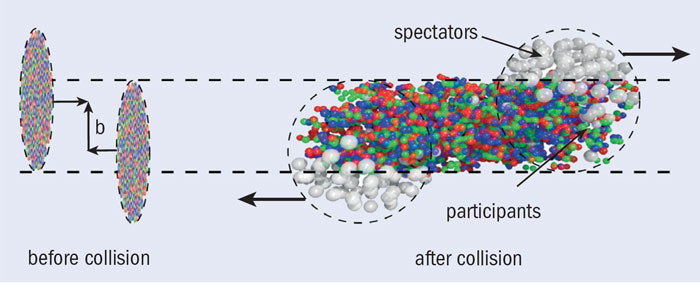
\includegraphics[width=1\textwidth]{Figures/spectatorsvsparticipants.jpg}
    \caption[Diagram showing impact parameter versus $N_{spectators}$ and $N_{participants}$]{Diagram showing impact parameter versus $N_{spectators}$ and $N_{participants}$\citep{cernhifireball}}
    \label{fig:cernfireball}
    \end{subfigure} 
    \rule{35em}{0.5pt}
    \begin{subfigure}[p]{0.7\textwidth}
    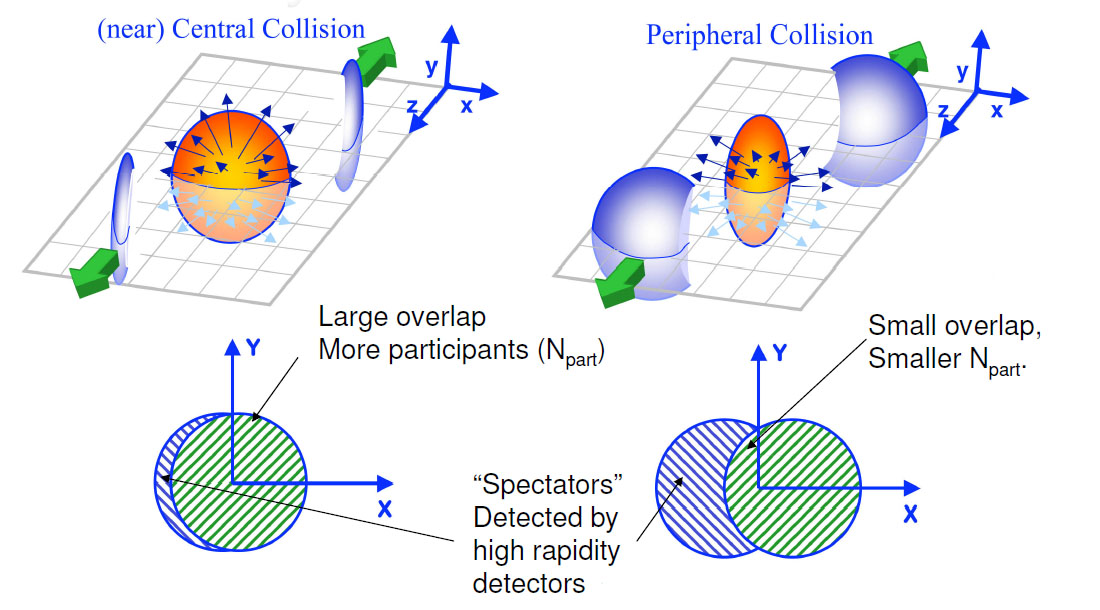
\includegraphics[width=1\textwidth]{Figures/centralvsperipheral.jpg}
	\caption[Central vs Peripheral collisions, geometry of initial conditions]{Central vs Peripheral collisions, geometry of initial conditions. The beam axis goes into and out of the page for the lower diagrams.}
\label{fig:centvsperiph}
    \end{subfigure}
    \rule{35em}{0.5pt}
\begin{subfigure}[p]{1\textwidth}
  \centering
    \includegraphics[width=0.5\textwidth]{prevplots/bbczdcanaresponse.JPG}

  \caption[Centrality bins as determined by ZDC energy versus BBC charge sum]{Centrality bins as determined by ZDC energy versus BBC charge sum\citep{Ghosh2001}. ZDC counts spectators, BBC counts particles produced by spectators, correlation of the two gives centrality parameter.}
  \label{fig:zdcvsbbc}
\end{subfigure}

    \rule{35em}{0.5pt}
  \caption[Central versus peripheral ion collisions, BBC vs ZDC determination of]{Central versus peripheral ion collisions, BBC vs ZDC determination of}
  \label{fig:centralvsperipheral}
\end{figure}


Extending the terminology from impact parameters, we then define a collision with a large number of participants to be a \textit{central} collision and a collision with a large number of spectators: a \textit{peripheral} collision. These are quantified in percents, 0$\%$ being most central collisions i.e. highest number of participants, $b=0$, two colliding ions overlap completely, and 100$\%$: ions completely miss each other, i.e. there are no participants, $b > R_{nucleus}$. Since ions are spherical in shape, centrality can be used as a way of describing the geometry of the collision region, central collisions have a more circular shape whereas peripheral collisions have a more almond-like shape. In practice, the asymmetric system of d+Au has spectators on the ``gold-going'' side. For this, BBC and ZDC correlations are done on the gold side and compared with the BBC (participant count) measurement on the deuteron side.



\subsection{Event Vertex and Timing}
\label{sect:timeandvtx}
The event vertex is the location along the beam axis where the collision happened relative to the equidistant point between the two beam beam counters. That is, an event vertex value of 0 would be exactly in the center of the PHENIX detector, at equal distance from both BBCs. When a collision happens, the non colliding nucleons (spectators) continue to travel through the interaction region and are detected at two different times, on the other side of the IR, by the two ZDCs (see fig \ref{fig:zdcvtx}). These two time measurements, $T_1$ and $T_2$ respectively, can be used to calculate both the event vertex ($z_{vtx}$) and the initial time the collision takes place ($T_0$) as follows\citep{Mitchell:2002wu}:

\begin{equation}
 z_{vtx} = \frac{T_1 - T_2}{2c} \qquad\text{and}\qquad T_0 = \frac{T_1 + T_2}{2}
\end{equation}

This initial time is used to start the stopwatch of the event and is used in conjunction with other detectors to to find the time a produced particle takes to travel from the vertex to a detector. The event vertex is used to determine if a collision happens in a region in the IR where a majority of created particle tracks will hit somewhere in the PHENIX acceptance. Too large of a vertex value and the collision is no longer happening in the ideal location for the central arms to detect outgoing tracks. The event vertex for the data set used in this analysis can be seen in figure \ref{fig:vtxdist} with an applied cut of $z_{vtx} \leq 30$ cm for optimal central arm track acceptance.

\begin{figure}[htbp!]
  \centering
    \includegraphics[width=1\textwidth]{Figures/BBCevtchar.JPG}
    \rule{35em}{0.5pt}
  \caption[Diagram of ZDC event characterization]{Diagram of ZDC event characterization. North and South ZDCs compare time measurements to determine the time of the start of the event and the vertex of the collision.}
  \label{fig:zdcvtx}
\end{figure}


\begin{figure}[htbp!]
  \centering
    \includegraphics[width=0.5\textwidth]{evtQA/zvtxdist.JPG}
    \rule{35em}{0.5pt}
  \caption[Event Vertex Distribution]{Event vertex distribution, there is an applied cut for all events to be $|z_{vtx}| \leq 30$ cm.}
  \label{fig:vtxdist}
\end{figure}

\section{Track Reconstruction}
\label{trkrecosect}
\subsection{Variables for Track Selection}
After the collision, created particles fly outward from the vertex and traverse the various layers of the PHENIX spectrometer, depositing information about their kinematics and species along the way. Due to the high multiplicity of tracks resulting from a heavy ion collision, there are a large number of hits in the various detectors that all must be matched to form coherent particle tracks. This high multiplicity makes it combinatorially difficult to come up with possible particle trajectories. The process of rejecting combinations of hits that are unlikely or are background and accepting hits is called \textit{track matching}. Track reconstruction is not perfect, not all hits can be correlated to a clean particle trajectory, and not all trajectories will deposit hits perfectly lined up in every detector subsystem. Therefore, it is important to come up with a metric with which to measure the quality of the tracks in order to discern which tracks have enough subsystem data to be reconstructed cleanly versus those which do not.
\subsubsection{Track Matching: DC and PC1}
Track reconstruction utilizes various layers of the Drift Chamber and Pad Chambers in concert to determine track momentum due to the varying curvature of tracks of different momenta traveling through a magnetic field. Tracks are reconstructed in the DC and PC1 using an algorithm called a \textit{combinatorial Hough Transform} (CHT)\citep{Mitchell:2002wu}. A CHT is a reconstruction algorithm used on a set of points that we know were created by single particles in order to fit them with likely linear track candidates\citep{OHLSSON199277}. The set of points are connected combinatorially and probabilities are assigned to each connection based on other kinematic variables and the likeliness that the connection describes a real particle track. For instance, we know all tracks must start at or reasonably close to the event vertex, therefore if any connected points point back to a point that we know is not the event vertex, it is unlikely that that connection reconstructs a real track created in the collision. Furthermore, further out from the vertex additional hits should happen at radially more distant detectors, and there should be corresponding points at those detectors as well.  We use a parameter called track \textit{quality} in order to quantify our confidence that a CHT reconstructed track is a likely fit. Track quality is a function of how many points in the different tracking detector layers were used to reconstruct a track. Since this is a combinatorial reconstruction, and since PHENIX doesn't exist in a vacuum, it is possible that other tracks such as cosmic events and background events are reconstructed.  Because of this we also make the assumption that the origin of all probable tracks is the event vertex as determined by the BBC. This analysis uses tracks whose accepted reconstructions were made with at least 3 hits in the inner tracking detectors (DC and PC): at least one hit in X1 and X2 wire nets in the DC(sect. \ref{sect:dcpc}) and a hit in PC1.

\begin{figure}[htbp!]
  \centering
    \includegraphics[width=0.7\textwidth]{Figures/houghtransformcartoon.JPG}
    \rule{35em}{0.5pt}
  \caption[Hits in the DC matched to tracks using a Hough transform]{Hits in the DC matched to tracks using a Hough transform. A CHT aims to provide these matched track lines by weighting combinatoric solutions with the probability of it being a physical track.}
  \label{fig:houghtransform}
\end{figure}

\subsubsection{Track Matching: TOF and PC3}
The magnetic field in PHENIX is strongest in the IR where $R<2 m$ and negilgible within the central arms\citep{rolnickthesis}. Therefore once tracks are matched in the DC and through the PC1 we can project the track linearly through the rest of the central arms. We can then match these projections with hits in the PC3 and TOF as illustrated in figure \ref{fig:pc3tofmatching} and assign variables (called \textit{residuals}) to the difference between where a hit landed in the TOF/PC3 versus where it was projected to be, one in azimuthal angle ($d\phi$) and one along beam axis ($dz$). Therefore, track purity can be increased by setting limits to how large a track's residuals can be. These residuals are set per strip in the TOFW (slat in the TOFE). DC/PC reconstructed track residuals for a given strip/slat are plotted and fit with a Gaussian. The corresponding width of this Gaussian is used to set the acceptance threshold for matched tracks projected out to the TOF/PC3. For this analysis, the maximum residual allowed for both TOF and PC3 in both $z$ and $\phi$ is three standard deviations ($3\sigma$) from the mean residual to allow for more statistics needed due to the lower multiplicity d+Au system (compared to larger systems) while still maintaining good track reconstruction purity. Combined with the DC/PC track quality cut, the TOF and PC3 matching cuts require that all reconstructed tracks used in this analysis be made with at least 5 points in 4 detector subsystems that are spread out over 5 m radially from the event vertex.
\begin{figure}[htbp!]
  \centering
    \includegraphics[width=0.9\textwidth]{Figures/pc3tofmatching.JPG}
    \rule{35em}{0.5pt}
  \caption[Diagram of track reconstruction by the DC/PC1 projected linearly onto the TOF/PC3]{Diagram of track reconstruction by the DC/PC1 projected linearly onto the TOF/PC3. \citep{schaeferthesis}}
  \label{fig:pc3tofmatching}
\end{figure}

\subsection{Particle Identification}
\label{sect:pidmethod}
Using the TOF detectors' high resolution timing measurements we are able to identify charged particles that are created in heavy ion collisions. For this analysis, the particles of interest are the charged pions ($\pi^{\pm}$), charged kaons ($k^{\pm}$), and protons/antiprotons ($p/\bar{p}$). Since the masses of these particles are distinct, plotting particle charge/momentum vs time of flight can show clear separation between pion, kaon, and proton signals (see fig \ref{fig:tofchargemom}). 

\begin{figure}[htbp!]
  \centering
    \includegraphics[width=0.7\textwidth]{Figures/tofchargemom.JPG}
    \rule{35em}{0.5pt}
  \caption[Particle separation in the TOF]{charge/momentum vs Time of Flight\citep{tofchargemom} is plotted to show particle separation in the TOF vis-\`a-vis equation \ref{eqn:qmomentum}. Pions, kaons, protons, and deuteron signals are labeled. Other signals corresponding to shorter flight times in the plot other particles, the closest to the pion signal are electrons, followed by photons which notably have a constant time of flight at all momenta (as they should).}
  \label{fig:tofchargemom}
\end{figure}

While visually the individual particle signatures are easily identifiable in this plot, computationally it is advantageous to convert units so that the signatures only depend on a single variable. We know from basic kinematics that we can calculate the velocity, v, of an object traveling at a constant speed:

\begin{equation}
v=\frac{L}{t} \implies t=\frac{L}{v},
\end{equation}
where t is the time it takes to travel some path length, L. It is useful to define the relative speed of the particle compared to the speed of light, c, as $\beta = v/c$ and substitute it in for v. We also know from the relativistic identities that $\beta = p/E$ and $E^{2} = p^{2} + m^{2}$. The equation is then: 

\begin{equation} \label{eqn:qmomentum}
t=\frac{L}{v} = t=\frac{L}{c\beta} = \frac{L}{c} \frac{E}{p} = \frac{L}{c} \frac{\sqrt{p^{2} + m^{2}}}{p}.
\end{equation}

which can be solved for $m^{2}$ to give the mass vs time relation:

\begin{equation} \label{eqn:m2tof}
m^{2} = p^{2} \bigg\{ \frac{t^{2}}{L^{2}} -1 \bigg\}.
\end{equation}

Since the distance from the event vertex to the detector is constant and the velocity (and therefore momentum) of the particle is constant, $m^{2}$ depends on two constant terms if we take measurements in bins of p. Since we are talking about radially outward traveling tracks, this p is, in practice, $p_{T}$. From this we can see that the time of flight for particles created in ion collisions can be used to identify their species.
\begin{figure}[htbp!]
  \centering
    \includegraphics[width=0.7\textwidth]{Figures/m2tofvspt.jpg}
    \rule{35em}{0.5pt}
  \caption[$m^{2}$ vs $p_{T}$ showing clear constant separation of particle signatures.]{$m^{2}$ vs $p_{T}$ showing clear constant separation of particle signatures.\citep{tofchargemom}. Under this transformation, electron peaks overlap strongly with pions and need to be cut out by using the RICH. Photons are massless leading to the wisp-like distribution for $m^2<0$.}
  \label{fig:m2tofvspt}
\end{figure}

\pagebreak
\pagebreak

% Chapter 4

\chapter{Anisotropic Flow} % Main chapter title
\label{sect:flow}
\section{Flow from Geometry of Initial Conditions}
%----------------------------------------------------------------------------------------
\begin{figure}[p]
  \centering
  \begin{subfigure}[h]{1\textwidth}
  \centering
    \includegraphics[width=0.6\textwidth]{Figures/pressuregradientsvscent.jpg}
    \caption{Symmetric systems (i.e. Au+Au, Pb+Pb, etc.).}
    \label{fig:pgradauau}
   \end{subfigure}
   \begin{subfigure}[h]{0.8\textwidth}
  \centering
    \includegraphics[width=0.6\textwidth]{Figures/pressuregradientsdau.jpg}
    \caption{Asymmetric systems. In this case (d+Au) the smaller ion is inherently elliptically shaped since it only contains two nucleons.}
   \label{fig:pgraddau}
   \end{subfigure}
        \rule{35em}{0.5pt}
  \caption[A cartoon showing pressure gradients in central versus peripheral collisions.]{Cartoons showing pressure gradients in central versus peripheral collisions in symmetric and asymmetric systems. Here the yellow and blue circles represent the colliding ions, one going into the page and one coming out of the page. The red circles denote surfaces of equal compression in the region of nucleon interaction. Peripheral collisions have the steepest gradient of compression along the event plane. Thus, an ellipsoidal ion collision anisotropy corresponds to a pressure anisotropy in the created medium leading to an elliptically shaped momentum anisotropy of flow which hadronizes and is measured as an azimuthal anisotropy of particles produced in the azimuth.}
  \label{fig:pressuregradients}
\end{figure}


In the moments immediately after a collision event, the outward expansion of the newly formed QGP can be studied to better understand the QCD processes that take place both during formation as well what happens as the temperature of the system drops to below the freeze out threshold. Though fluctuations in collision geometry can happen, if we ignore them for the moment, we can say that the shape of the colliding ions' cross-sectional overlap provides a good approximation of the initial conditions of the medium after collision. Therefore, the geometry of the initial configuration of participants is dependent on the collision's centrality\footnote{see sect. \ref{sect:centrality}}. Because of this, peripheral events in symmetric systems such as Au+Au have an inherently elliptical shape (as shown in figure \ref{fig:pgradauau}). The azimuthal asymmetry of this interaction creates different amounts of pressure, or \textit{pressure gradients}, about the azimuth. These pressures are strongest along the waist of the collision and weakest at the poles. Because of this, though it expands in all directions, it is the stronger expansion about the azimuth that best describes the behavior of this fluid. Asymmetric systems, such as the one studied in this analysis (d+Au), have a different dependence on centrality. As shown in figure \ref{fig:pgraddau}, since deuterons contain only two nucleons, they are inherently elliptical in shape, the pressure gradients then only depend on how many of the gold ion's nucleons the deuteron interacts with. By the Glauber model, we can approximate the nucleon distribution of an ion as a density function that decreases with increasing radius. Therefore, it follows that, for d+Au, pressure gradients are maximal with central collisions since nuclear interaction is maximal at maximum centrality. Consequently, flow should be strongest in central collisions due to this maximal pressure.  

Often physicists like to describe the behavior of phenomena using a series expansion of orthogonal functions. Since the azimuthal angle runs from $0$ to $2 \pi$, this azimuthal expansion can be treated as a harmonic function which lends itself well to parameterization using a Fourier series. Recall that a Fourier series can be used to approximate the shape of a periodic function, $f(x)$, over a fixed period, $L$:

\begin{equation}
f(x) = \sum^{\infty}_{n=-\infty} A_{n} e^{i(2 \pi n x / L)}
\end{equation}
where
\begin{equation}
A_{n} = \frac{1}{L} \int^{L}_{0} f(\phi) e^{-i(2 \pi n x / L)} dx
\end{equation}

are said to be the Fourier \textbf{coefficients} or often, since they approximate harmonic functions, Fourier \textbf{harmonics}. For azimuthal periodicity, $L=2\pi$ and these equations become: 

\begin{equation}
f(\phi) = \sum^{\infty}_{n=-\infty} A_{n} e^{i(n \phi)}
\end{equation}
where
\begin{equation}
A_{n} = \frac{1}{2\pi} \int^{-\pi}_{\pi} f(\phi) e^{-i(n \phi)} d\phi
\end{equation}

These coefficients describe the amount a particular harmonic's functional shape contributes to the overall shape of the periodic function. We know that the exponential term can be written as the sum of a real cosine term and an imaginary sine term:

\begin{equation}
f(\phi) = \sum^{\infty}_{n=0} A_{n} cos ( n \phi) + i \sum^{\infty}_{n=0} B_{n} sin (n \phi)
\end{equation}
where
\begin{equation}
A_{n} = \frac{1}{2\pi} \int^{-\pi}_{\pi} f(\phi) cos (n \phi) d\phi
\end{equation}
and
\begin{equation}
B_{n} = \frac{1}{2\pi} \int^{-\pi}_{\pi} f(\phi) sin (n \phi) d\phi 
\end{equation}

\begin{figure}[htbp!]
  \centering
  \rule{35em}{0.5pt}
    \includegraphics[width=0.7\textwidth]{Figures/RP_InOutPlane_3.jpg}
        
  \caption[Reaction plane coordinates.]{Reaction plane coordinates. $\phi = 0$ is oriented along the reaction plane therefore track vectors with $\Delta\phi$ values at $\pi/2$ and $3 \pi / 2$ correspond to particles produced out of the event plane and $\Delta\phi$ values of $0$ and $\pi$ correspond to vectors in the event plane.}
  \rule{35em}{0.5pt}
  \label{fig:dphiep}
\end{figure}


Since we define $\phi=0$ to be along the waist of the ellipsoidal shaped QGP and not at the poles (see fig \ref{fig:dphiep}), odd function contributions (sine terms, $B_{n}$) to the Fourier series can all be ignored. Therefore, if we wish to approximate the shape of the outgoing flow from the QGP, we can define the rate of change of outgoing particle tracks vs transverse momentum and approximate it with a Fourier series. Flow anisotropy of the QGP can then be written as:
\begin{equation}
E \frac{d^{3}N}{dp^{3}} = \frac{1}{2 \pi} \frac{d^{2}N}{p_{T} dp_{T}dy}\Big( 1 + \sum^{\infty}_{n=1} 2 v_{n} \cos\big(n \Delta \phi)\big) \Big),
\end{equation}
where:
\begin{equation}
v_{n} = \bigg \langle cos \Big( n \Delta\phi \Big) \bigg \rangle
\end{equation}
are the n-th order Fourier coefficients that describe the azimuthal shape of the QGP's outward expansion and $\Delta \phi = \phi_{lab} - \Psi_{RP}$ is the azimuthal angle with respect to the reaction plane angle relative measured in the lab coordinate system, changing the lab coordinate phi to the angle phi with respect to the event plane. Each n-th order coefficient scales the amount of expansion that behaves like $cos$ $nx$.

\begin{figure}[htbp!]
  \centering
    \includegraphics[width=0.8\textwidth]{Figures/fouriercosines.jpg}
    \rule{35em}{0.5pt}
  \caption[Plots of the first four harmonics of a cosine series.]{Plots of the first four harmonics of a cosine series. $\phi=0$ is along the event plane and increasing $\phi$ goes clockwise as shown in figure \ref{fig:dphiep}.}
  \label{fig:fouriercosines}
\end{figure}

From studying the behavior of these various harmonics we can see that $n=0$ corresponds to a constant term since $\cos{0} = 1$ for $n=1$. Furthermore, $\cos{x}$ is a maximum at $\phi=0$ and a minimum at $\phi = \pi$ which would correspond to a collective flow in the $\phi=0$ direction. Therefore, the $n=1$ flow coefficient is often called \textit{directed flow}. For the case of $n=2$ we see that again there is a maximum at $\phi=0$ and another at $\phi=\pi$ which corresponds to maximal flow along the event plane of the ellipsoidal QGP. This anisotropic expansion that is strongest along the reaction plane in an elliptical collective flow, a term which is shortened to \textit{elliptic flow}. There are higher order harmonics which can describe various other phenomena of QGP flow which are beyond the scope of this analysis.

\section{Flow from Fluctuations}
Geometric sources of initial conditions are a good approximation; however, it has been seen that higher harmonics can be measured in elliptic systems such as peripheral Au+Au previously thought to be only elliptic\citep{Alver:2010gr}. This effect has been attributed to secondary scattering processes of the participant nucleons. These nucleons that interact with spectators in secondary reactions are called \textit{wounded nucleons} and the overall effect of these additional collisions increases both the number of binary collisions and alters the initial shape of the created medium. An example of this shown in figure \ref{fig:v3inauau} where a symmetric Au+Au system collided peripherally and we expect a strong $v_2$, however fluctuations and wounded nucleons create a triangular shaped initial condition, which would correspond to a $v_3$ signal.

\begin{figure}[htbp!]
  \centering
    \includegraphics[width=0.8\textwidth]{prevplots/phobosglauberv3.JPG}
    \rule{35em}{0.5pt}
  \caption[Triangular Flow from Fluctuations.]{An example of how fluctuations can cause flow with the shape of higher Fourier harmonics. Here Au+Au collisions are modeled with Glauber Monte Carlo. The distribution of nucleons at the point of collision in the x-y plane is plotted. Wounded nucleons cause secondary collisions which alter the initial elliptic shape from the overlap into a triangular shape\citep{Alver:2010gr}. In this plot small dotted circles are spectators and solid circles are participants, the large dotted circle that contains the various circles are outlines of the two colliding ions.}
  \label{fig:v3inauau}
\end{figure}
\pagebreak
\pagebreak

% Chapter 6

\chapter{Event Plane} % Main chapter title

\section{Determination of Event Plane}
\section{Event Plane "Flattening"}
\section{Event Plane Resolution Correction}
So we correct this resolution error by some multiplicative scaling such that:
\begin{equation}
v_2^{res corr} = \frac{\langle cos (2(\phi - \Psi_2)) \rangle}{Res(\Psi_2)}
\end{equation}
where $\phi$ is the azimuthal angle, $\Psi_2$ is the 2nd order Fourier harmonic event plane, and $Res(\Psi_2)$ is a single valued correction factor for a $v_2$ measurement using a specific detector and a single bin in centrality. Since device resolution is independent of particle species, we do not need to calculate a different correction for each particle flow. 

The method used for this analysis is called the \textit{Three Subevent Method} and can be calculated by comparing the event plane measured with one detector to measurements made by two other detectors.
%----------------------------------------------------------------------------------------
\begin{equation}
Res\{2k \Psi^{A}\} = \sqrt{\frac{\langle cos(2k[\Psi^{A}-\Psi^{B}])\rangle \langle cos(2k[\Psi^{A}-\Psi^{C}])\rangle}{\langle cos(2k[\Psi^{B}-\Psi^{C}])\rangle}}
\end{equation} 
\pagebreak
\pagebreak

% Chapter 6

\chapter{Results} % Main chapter title
\section{Charged Track $v_{2}$}
Here I present measurements of elliptic flow in $\sqrt{s_{NN}}=200$ GeV d+Au collisions. Since the flattening the event plane redistributes the event plane distribution, the unidentified charged track flow can be measured directly from plots of $d\phi$. Recall that the Fourier coefficients parameterize the shape of the azimuthal hydrodynamic flow by describing it as a superposition of cosine harmonics:
\begin{equation}
\frac{d^{2}N}{dp^{2}} \propto v_0 + v_1 \cos\big(\phi - \Psi_{r}\big) + v_2 \cos\big(2(\phi - \Psi_{r})\big) + v_3 \cos\big(3(\phi - \Psi_{r})\big) \cdots
\end{equation}
where $v_0$, $v_1$, $v_2$, and $v_3$ are the values that scale the amount of spherical, directed, elliptic, and triangular flow respectively, and are indicative of collective behavior of the nuclear matter. To measure the elliptic flow we count number of tracks in bins of $d\phi$ and fit this with a function of the form:
\begin{equation}
\label{v2fitfn}
f(x) = A [1 + B \cos 2x]
\end{equation}
where A is a term that accounts for an overall shift in the number of tracks due to statistics and B is our $v_2$. Due to the asymmetric nature of d+Au collisions, event plane calculations are significantly better on the Au going side, because of this, the following plots (figures \ref{fig:Ndphicent0}-\ref{fig:Ndphicent3}) were made using the BBC South determination of the event plane. They are binned in 5\% bins of centrality up to 15\%, at which point statistics requires the remainder of data to be binned 10\%-25\%. This $d\phi$ plot can then be fit with the aforementioned cosine function to calculate the elliptic flow measurements vs centrality for all charged tracks which is shown in figure \ref{fig:alltrackv2}.


\begin{figure}[htbp!]
  \centering
    \includegraphics[width=1\textwidth]{chargedtrackv2/htrkdphi2bbcs_0.jpg}
    \rule{35em}{0.5pt}
  \caption[$\frac{dN}{d\phi}$ vs $d\phi$, 0-5\% centrality.]{$\frac{d^N}{d\phi}$ vs $d\phi$, 0-5\% centrality, each plot represents a 0.2 GeV slice in transverse momentum space.}
  \label{fig:Ndphicent0}
\end{figure}

\begin{figure}[htbp!]
  \centering
    \includegraphics[width=1\textwidth]{chargedtrackv2/htrkdphi2bbcs_1.jpg}
    \rule{35em}{0.5pt}
  \caption[$\frac{dN}{d\phi}$ vs $d\phi$, 5-10\% centrality.]{$\frac{d^N}{d\phi}$ vs $d\phi$, 5-10\% centrality, each plot represents a 0.2 GeV slice in transverse momentum space.}
  \label{fig:Ndphicent1}
\end{figure}
\begin{figure}[htbp!]
  \centering
    \includegraphics[width=1\textwidth]{chargedtrackv2/htrkdphi2bbcs_2.jpg}
    \rule{35em}{0.5pt}
  \caption[$\frac{dN}{d\phi}$ vs $d\phi$, 10-15\% centrality.]{$\frac{d^N}{d\phi}$ vs $d\phi$, 10-15\% centrality, each plot represents a 0.2 GeV slice in transverse momentum space.}
  \label{fig:Ndphicent2}
\end{figure}
\begin{figure}[htbp!]
  \centering
    \includegraphics[width=1\textwidth]{chargedtrackv2/htrkdphi2bbcs_3.jpg}
    \rule{35em}{0.5pt}
  \caption[$\frac{dN}{d\phi}$ vs $d\phi$, 15-25\% centrality.]{$\frac{d^N}{d\phi}$ vs $d\phi$, 15-25\% centrality, each plot represents a 0.2 GeV slice in transverse momentum space.}
  \label{fig:Ndphicent3}
\end{figure}

\begin{figure}[htbp!]
  \centering
    \includegraphics[width=0.7\textwidth]{chargedtrackv2/rawtrackv2_bbcNS.jpg}
    \rule{35em}{0.5pt}
  \caption[Charged track elliptic flow,$\sqrt{s_{NN}}=$200 GeV d+Au collisions]{Charged track elliptic flow,$\sqrt{s_{NN}}=$200 GeV d+Au collisions}
  \label{fig:alltrackv2}
\end{figure}
\clearpage
\section{Separating Particle Signals}
Following the flattening of the event plane and checking for calibration of the TOF detector, I can plot a 2-d histogram of $p_T$ vs $m^2$ following the method described in section \ref{sect:pidmethod} to identify the species of charged track hits in the TOF. In order to do a statistical analysis, these 2-d histograms will need to be ``sliced'' into a series of 1-d histograms in small bins of $p_T$ which will give a 3-peak histogram showing the signatures of the pion, kaon, and proton which are Gaussian in shape. The widths and heights of these particle peaks will change and overlap in various ways over the variance of $p_t$, because of this I will divide the $p_T$ range into three ranges which will be analyzed with different methods. The Gaussians are then integrated to calculate the particle yield for each species. Integration bounds can be set to increase track ID purity at the expense of statistics and vice versa. As a QA tool means and widths across each bin in $d\phi$ are plotted and set to be flat as there should not be a shift in either of those for a set bin of $p_T$. The yields from the integrated Gaussians are then fit with the Fourier function to determine the 2nd harmonic coefficient as per equation \ref{v2fitfn}.

\subsection{Single Gaussians}
For $p_T< 1.3$, there is enough separation between the pion, kaon, and proton signals to fit each particle peak with a single Gaussian. This will take the form:
\begin{equation}
f(x) = \frac{N_0}{\sqrt{2\pi \sigma^2}} e^{-\frac{(x-\mu)^2}{2\sigma^{2}}},
\end{equation}
where $\sigma$ is the width of the identified particle peak, $\mu$ is the location of the peak's mean along the x-axis, and $N_0$ is the height of the peak. The Gaussians are then integrated from $\mu-2\sigma$ to $\mu+2\sigma$ for each particle distribution, i.e. the number of particles of each type are counted out to two standard deviations around their mean mass. 

\newgeometry{top=2cm} 
\subsubsection{Single Gaussian fits, $p_T$=0.5-1.3 GeV/c, TOF.W, negative charged tracks}

\begin{figure}[H]
  \centering
    \begin{subfigure}{1\textwidth}
    \includegraphics[width=1\textwidth]{lowptfits/yieldvsdphi_tof1_cent0_ch0_pT-5-7.jpg}
    \end{subfigure}
    \begin{subfigure}{1\textwidth}
    \includegraphics[width=1\textwidth]{lowptfits/fitParams_tof1_cent0_ch0_pT-5-7.jpg}
    \end{subfigure}
    \rule{35em}{0.5pt}
  \caption[PID fits and Yield vs $d\phi$ for $p_T$=0.5-0.7 GeV/c, TOF.W, negative particles ]{$m^2$ Gaussian fits for PID and resulting Yield vs $d\phi$ for $p_T$=0.5-0.7 GeV/c, TOF.W, negative particles}
  \label{fig:fits5-7neg}
\end{figure}

\begin{figure}[H]
  \centering
    \begin{subfigure}{1\textwidth}
    \includegraphics[width=1\textwidth]{lowptfits/yieldvsdphi_tof1_cent0_ch0_pT-7-9.jpg}
    \end{subfigure}
    \begin{subfigure}{1\textwidth}
    \includegraphics[width=1\textwidth]{lowptfits/fitParams_tof1_cent0_ch0_pT-7-9.jpg}
    \end{subfigure}
    \rule{35em}{0.5pt}
  \caption[PID fits and Yield vs $d\phi$ for $p_T$=0.7-0.9 GeV/c, TOF.W, negative particles ]{$m^2$ Gaussian fits for PID and resulting Yield vs $d\phi$ for $p_T$=0.7-0.9 GeV/c, TOF.W, negative particles}
  \label{fig:fits7-9neg}
\end{figure}

\begin{figure}[H]
  \centering
    \begin{subfigure}[p]{1\textwidth}
    \includegraphics[width=1\textwidth]{lowptfits/yieldvsdphi_tof1_cent0_ch0_pT-9-11.jpg}
    \end{subfigure}
    \begin{subfigure}[p]{1\textwidth}
    \includegraphics[width=1\textwidth]{lowptfits/fitParams_tof1_cent0_ch0_pT-9-11.jpg}
    \end{subfigure}
    \rule{35em}{0.5pt}
  \caption[PID fits and Yield vs $d\phi$ for $p_T$=0.9-1.1 GeV/c, TOF.W, negative particles ]{$m^2$ Gaussian fits for PID and resulting Yield vs $d\phi$ for $p_T$=0.9-1.1 GeV/c, TOF.W, negative particles}
  \label{fig:fits9-11neg}
\end{figure}

\begin{figure}[H]
  \centering
    \begin{subfigure}[p]{1\textwidth}
    \includegraphics[width=1\textwidth]{lowptfits/yieldvsdphi_tof1_cent0_ch0_pT-11-13.jpg}
    \end{subfigure}
    \begin{subfigure}[p]{1\textwidth}
    \includegraphics[width=1\textwidth]{lowptfits/fitParams_tof1_cent0_ch0_pT-11-13.jpg}
    \end{subfigure}
    \rule{35em}{0.5pt}
  \caption[PID fits and Yield vs $d\phi$ for $p_T$=1.1-1.3 GeV/c, TOF.W, negative particles ]{$m^2$ Gaussian fits for PID and resulting Yield vs $d\phi$ for $p_T$=1.1-1.3 GeV/c, TOF.W, negative particles}
  \label{fig:fits11-13neg}
\end{figure}

\subsubsection{Single Gaussian fits, $p_T$=0.5-1.3 GeV/c, TOF.W, positive charged tracks}

\begin{figure}[H]
  \centering
    \begin{subfigure}[p]{1\textwidth}
    \includegraphics[width=1\textwidth]{lowptfits/yieldvsdphi_tof1_cent0_ch1_pT-5-7.jpg}
    \end{subfigure}
    \begin{subfigure}[p]{1\textwidth}
    \includegraphics[width=1\textwidth]{lowptfits/fitParams_tof1_cent0_ch1_pT-5-7.jpg}
    \end{subfigure}
    \rule{35em}{0.5pt}
  \caption[PID fits and Yield vs $d\phi$ for $p_T$=0.5-0.7 GeV/c, TOF.W, positive particles ]{$m^2$ Gaussian fits for PID and resulting Yield vs $d\phi$ for $p_T$=0.5-0.7 GeV/c, TOF.W, positive particles}
  \label{fig:fits5-7pos}
\end{figure}

\begin{figure}[H]
  \centering
    \begin{subfigure}[p]{1\textwidth}
    \includegraphics[width=1\textwidth]{lowptfits/yieldvsdphi_tof1_cent0_ch1_pT-7-9.jpg}
    \end{subfigure}
    \begin{subfigure}[p]{1\textwidth}
    \includegraphics[width=1\textwidth]{lowptfits/fitParams_tof1_cent0_ch1_pT-7-9.jpg}
    \end{subfigure}
    \rule{35em}{0.5pt}
  \caption[PID fits and Yield vs $d\phi$ for $p_T$=0.7-0.9 GeV/c, TOF.W, positive particles ]{$m^2$ Gaussian fits for PID and resulting Yield vs $d\phi$ for $p_T$=0.7-0.9 GeV/c, TOF.W, positive particles}
  \label{fig:fits7-9pos}
\end{figure}

\begin{figure}[H]
  \centering
    \begin{subfigure}[p]{1\textwidth}
    \includegraphics[width=1\textwidth]{lowptfits/yieldvsdphi_tof1_cent0_ch1_pT-9-11.jpg}
    \end{subfigure}
    \begin{subfigure}[p]{1\textwidth}
    \includegraphics[width=1\textwidth]{lowptfits/fitParams_tof1_cent0_ch1_pT-9-11.jpg}
    \end{subfigure}
    \rule{35em}{0.5pt}
  \caption[PID fits and Yield vs $d\phi$ for $p_T$=0.9-1.1 GeV/c, TOF.W, positive particles ]{$m^2$ Gaussian fits for PID and resulting Yield vs $d\phi$ for $p_T$=0.9-1.1 GeV/c, TOF.W, positive particles}
  \label{fig:fits9-11pos}
\end{figure}

\begin{figure}[H]
  \centering
    \begin{subfigure}[p]{1\textwidth}
    \includegraphics[width=1\textwidth]{lowptfits/yieldvsdphi_tof1_cent0_ch1_pT-11-13.jpg}
    \end{subfigure}
    \begin{subfigure}[p]{1\textwidth}
    \includegraphics[width=1\textwidth]{lowptfits/fitParams_tof1_cent0_ch1_pT-11-13.jpg}
    \end{subfigure}
    \rule{35em}{0.5pt}
  \caption[PID fits and Yield vs $d\phi$ for $p_T$=1.1-1.3 GeV/c, TOF.W, positive particles ]{$m^2$ Gaussian fits for PID and resulting Yield vs $d\phi$ for $p_T$=1.1-1.3 GeV/c, TOF.W, positive particles}
  \label{fig:fits11-13pos}
\end{figure}
\restoregeometry


\subsection{Gaussian Mixing}
For $1.3<p_T<2.1$, kaon and pion mass distributions become overlapped. To decouple the two I use a mixed Gaussian model in order to fit the tails of the distributions without over counting. This function takes the form:

\begin{equation}
f(x) = \frac{1}{\sqrt{2\pi}} \bigg( \frac{N_{\pi}}{\sigma_{\pi}} e^{-\frac{(x-\mu_{\pi})^2}{2\sigma_{\pi}^{2}}} + \frac{N_{k}}{\sigma_{\pi}-\sigma_{k}} e^{-\frac{(x-\mu_{k})^2}{2(\sigma_{\pi} - \sigma_{k})^{2}}} \bigg),
\end{equation}
where $N_{x}$, $\mu_x$, and $\sigma_x$ are the parameters that describe the shape of particle $x$'s ($\pi$/k) distribution. These parameters can then be used to reconstruct single Gaussian distributions which are then integrated out to $2\sigma$ as mentioned in the previous section.

\newgeometry{top=2cm} 
\subsubsection{Mixed Gaussian fits, $p_T$=1.3-2.1 GeV/c, TOF.W, negative charged tracks}

\begin{figure}[H]
  \centering
    \begin{subfigure}{1\textwidth}
    \includegraphics[width=1\textwidth]{lowptfits/yieldvsdphi_tof1_cent0_ch0_pT-13-15.jpg}
    \end{subfigure}
    \begin{subfigure}{1\textwidth}
    \includegraphics[width=1\textwidth]{lowptfits/fitParams_tof1_cent0_ch0_pT-13-15.jpg}
    \end{subfigure}
    \rule{35em}{0.5pt}
  \caption[PID fits and Yield vs $d\phi$ for $p_T$=1.3-1.5 GeV/c, TOF.W, negative particles ]{$m^2$ Gaussian fits for PID and resulting Yield vs $d\phi$ for $p_T$=1.3-1.5 GeV/c, TOF.W, negative particles}
  \label{fig:fits13-15neg}
\end{figure}

\begin{figure}[H]
  \centering
    \begin{subfigure}{1\textwidth}
    \includegraphics[width=1\textwidth]{lowptfits/yieldvsdphi_tof1_cent0_ch0_pT-15-17.jpg}
    \end{subfigure}
    \begin{subfigure}{1\textwidth}
    \includegraphics[width=1\textwidth]{lowptfits/fitParams_tof1_cent0_ch0_pT-15-17.jpg}
    \end{subfigure}
    \rule{35em}{0.5pt}
  \caption[PID fits and Yield vs $d\phi$ for $p_T$=1.5-1.7 GeV/c, TOF.W, negative particles ]{$m^2$ Gaussian fits for PID and resulting Yield vs $d\phi$ for $p_T$=1.5-1.7 GeV/c, TOF.W, negative particles}
  \label{fig:fits15-17neg}
\end{figure}

\begin{figure}[H]
  \centering
    \begin{subfigure}[p]{1\textwidth}
    \includegraphics[width=1\textwidth]{lowptfits/yieldvsdphi_tof1_cent0_ch0_pT-17-19.jpg}
    \end{subfigure}
    \begin{subfigure}[p]{1\textwidth}
    \includegraphics[width=1\textwidth]{lowptfits/fitParams_tof1_cent0_ch0_pT-17-19.jpg}
    \end{subfigure}
    \rule{35em}{0.5pt}
  \caption[PID fits and Yield vs $d\phi$ for $p_T$=1.7-1.9 GeV/c, TOF.W, negative particles ]{$m^2$ Gaussian fits for PID and resulting Yield vs $d\phi$ for $p_T$=1.7-1.9 GeV/c, TOF.W, negative particles}
  \label{fig:fits17-19neg}
\end{figure}

\begin{figure}[H]
  \centering
    \begin{subfigure}[p]{1\textwidth}
    \includegraphics[width=1\textwidth]{lowptfits/yieldvsdphi_tof1_cent0_ch0_pT-19-21.jpg}
    \end{subfigure}
    \begin{subfigure}[p]{1\textwidth}
    \includegraphics[width=1\textwidth]{lowptfits/fitParams_tof1_cent0_ch0_pT-19-21.jpg}
    \end{subfigure}
    \rule{35em}{0.5pt}
  \caption[PID fits and Yield vs $d\phi$ for $p_T$=1.9-2.1 GeV/c, TOF.W, negative particles ]{$m^2$ Gaussian fits for PID and resulting Yield vs $d\phi$ for $p_T$=1.9-2.1 GeV/c, TOF.W, negative particles}
  \label{fig:fits19-21neg}
\end{figure}

\subsubsection{Mixed Gaussian fits, $p_T$=1.3-2.1 GeV/c, TOF.W, positive charged tracks}

\begin{figure}[H]
  \centering
    \begin{subfigure}[p]{1\textwidth}
    \includegraphics[width=1\textwidth]{lowptfits/yieldvsdphi_tof1_cent0_ch1_pT-13-15.jpg}
    \end{subfigure}
    \begin{subfigure}[p]{1\textwidth}
    \includegraphics[width=1\textwidth]{lowptfits/fitParams_tof1_cent0_ch1_pT-13-15.jpg}
    \end{subfigure}
    \rule{35em}{0.5pt}
  \caption[PID fits and Yield vs $d\phi$ for $p_T$=1.3-1.5 GeV/c, TOF.W, positive particles ]{$m^2$ Gaussian fits for PID and resulting Yield vs $d\phi$ for $p_T$=1.3-1.5 GeV/c, TOF.W, positive particles}
  \label{fig:fits13-15pos}
\end{figure}

\begin{figure}[H]
  \centering
    \begin{subfigure}[p]{1\textwidth}
    \includegraphics[width=1\textwidth]{lowptfits/yieldvsdphi_tof1_cent0_ch1_pT-15-17.jpg}
    \end{subfigure}
    \begin{subfigure}[p]{1\textwidth}
    \includegraphics[width=1\textwidth]{lowptfits/fitParams_tof1_cent0_ch1_pT-15-17.jpg}
    \end{subfigure}
    \rule{35em}{0.5pt}
  \caption[PID fits and Yield vs $d\phi$ for $p_T$=1.5-1.7 GeV/c, TOF.W, positive particles ]{$m^2$ Gaussian fits for PID and resulting Yield vs $d\phi$ for $p_T$=1.5-1.7 GeV/c, TOF.W, positive particles}
  \label{fig:fits15-17pos}
\end{figure}

\begin{figure}[H]
  \centering
    \begin{subfigure}[p]{1\textwidth}
    \includegraphics[width=1\textwidth]{lowptfits/yieldvsdphi_tof1_cent0_ch1_pT-17-19.jpg}
    \end{subfigure}
    \begin{subfigure}[p]{1\textwidth}
    \includegraphics[width=1\textwidth]{lowptfits/fitParams_tof1_cent0_ch1_pT-17-19.jpg}
    \end{subfigure}
    \rule{35em}{0.5pt}
  \caption[PID fits and Yield vs $d\phi$ for $p_T$=1.7-1.9 GeV/c, TOF.W, positive particles ]{$m^2$ Gaussian fits for PID and resulting Yield vs $d\phi$ for $p_T$=1.7-1.9 GeV/c, TOF.W, positive particles}
  \label{fig:fits17-19pos}
\end{figure}

\begin{figure}[H]
  \centering
    \begin{subfigure}[p]{1\textwidth}
    \includegraphics[width=1\textwidth]{lowptfits/yieldvsdphi_tof1_cent0_ch1_pT-19-21.jpg}
    \end{subfigure}
    \begin{subfigure}[p]{1\textwidth}
    \includegraphics[width=1\textwidth]{lowptfits/fitParams_tof1_cent0_ch1_pT-19-21.jpg}
    \end{subfigure}
    \rule{35em}{0.5pt}
  \caption[PID fits and Yield vs $d\phi$ for $p_T$=1.9-2.1 GeV/c, TOF.W, positive particles ]{$m^2$ Gaussian fits for PID and resulting Yield vs $d\phi$ for $p_T$=1.9-2.1 GeV/c, TOF.W, positive particles}
  \label{fig:fits19-21pos}
\end{figure}
\restoregeometry

\subsection{ACC as a Particle Discriminator}
Above $p_T=2.3$ pion/kaon mixing becomes inseparable. In this region I utilize the ACC to trigger and veto pion and kaon events respectively by setting Cherenkov radiation threshold which is done by counting the number of photoelectrons collected by the two PMTs on each channel of the ACC. This utilization of the ACC therefore sorts tracks into two separate histograms, one with an \textit{ACC fire} condition that contains mostly pions with minimal kaon contamination, and another with an \textit{ACC veto} condition that contains the remaining kaons and protons with minimal pion contamination. These two histograms can then be analyzed with single Gaussians since the distributions are now separate. This ACC threshold is the sum of the number of photoelectrons ($N_{p.e.}$) in both PMTs. The total number of $N_{p.e.}$ is plotted versus $m^2$ in a 2-d histogram and a threshold is set in order for there to be a maximum separation between pion and kaon signals. This 2-d histogram is then projected from the threshold up to the highest $N_{p.e.}$ bin for the pions and projected from the threshold down to the lowest $N_{p.e.}$ bin for kaons and protons. These 1-d projections can then be modeled with either single Gaussians (pions) or mixed Gaussians (kaons and protons).

\newgeometry{top=2cm} 
\subsubsection{TOF.W and ACC, $p_T$=2.1-3.5 GeV, negative charged tracks}

\begin{figure}[H]
  \centering
    \begin{subfigure}{1\textwidth}
    \includegraphics[width=1\textwidth]{hiptfits/neg/PSaccthreshold_cent0_ich0_accfire0_ptbin8.jpg}
    \caption{$N_{p.e.}$ vs $m^2$}
    \end{subfigure}
    \begin{subfigure}{1\textwidth}
    \includegraphics[width=1\textwidth]{hiptfits/neg/PSm2_cent0_ich0_accfire0_ptbin8.jpg}
    \caption{$m^2$ for ACC vetoed tracks}
    \end{subfigure}
  \label{fig:fits13-15neg}
\end{figure}

\begin{figure}[H]
  \ContinuedFloat
    \begin{subfigure}{1\textwidth}
    \includegraphics[width=1\textwidth]{hiptfits/neg/PSm2_cent0_ich0_accfire1_ptbin8.jpg}
    \caption{$m^2$ for ACC fired tracks}
    \end{subfigure}  
    \begin{subfigure}{1\textwidth}
    \includegraphics[width=1\textwidth]{hiptfits/neg/fitParams_tof2_cent0_ch0_pT-21-23.jpg}
    \caption{$m^2$ for ACC fired tracks}
    \end{subfigure}    
    \rule{35em}{0.5pt}
  \caption[PID fits and Yield vs $d\phi$ for $p_T$=1.3-1.5 GeV/c, TOF.W, negative particles ]{$m^2$ Gaussian fits for PID and resulting Yield vs $d\phi$ for $p_T$=1.3-1.5 GeV/c, TOF.W, negative particles}
  \label{fig:fits13-15neg}
\end{figure}
\restoregeometry

\subsection{High $p_T$: Fixed Width and Mean}

\section{Yield vs Event Plane}
Here the yield vs $d\phi$ plots can be treated like the $dN/d\phi$ vs $d\phi$ plots that provided the charged track $v_2$ measurement which was acquired by fitting with the functional form of equation \ref{v2fitfn}. 
\section{Identified Particle $v_{2}$}

\pagebreak
\pagebreak

% Chapter 7

\chapter{Error Analysis} % Main chapter title
There are various sources of systematic error that could contribute to uncertainty in this measurement. These include certainty in how the event plane was determined (sect. \ref{secteperr}), how well the event centrality can be determined (sect. \ref{sectcenterr}), various uncertainties pertaining to the identification of the particles (sect. \ref{sectpiderr}), and the effects of detector acceptance (sect. \ref{sectaccepterr}). In this chapter I will quantify the uncertainty for each of these contributions and then use these values to find the possible variance in the flow measurement due to these uncertainties. It will be shown that event plane resolution and PID systematics due to Gaussian fitting dominate and other errors are negligible.

Any uncertainty that would affect the value of this flow measurement would do so in one of two ways: either by shifting individual $v_2$ data points (changing inherent shape of the data set) or by changing the overall scaling of the whole measurement in a net direction (simple scaling of entire data set). Errors that would simply shift all values of $v_2$ are the event plane resolution and centrality determination errors. Errors that would shift individual points consist of the various PID uncertainties and detector acceptance effects. The way the uncertainties in this category would shift individual data points is by changing the shape of the particle yield distribution in $d\phi$. Recall that there are two terms that parametrize the shape of the yield in $d\phi$:

\begin{equation}
yield(d\phi) = v_0 [1 + v_2 \cos 2d\phi]
\end{equation}

In this equation, $v_0$ corresponds to an overall shift in the function, that is to say it describes the up-and-down displacement of the whole curve and doesn't affect the general shape of it. The remaining parameter, $v_2$, describes the shape of the yield distribution in $d\phi$. Changes to the shape of this distribution happen when yield values are perturbed up or down in individual bins of $d\phi$ which results in a change in the associated $v_2$ . In order to study the strength of $v_2$-affecting uncertainties I will apply the variances discussed in this chapter to individual points in the yield vs $d\phi$ distribution and re-fit in order to see the variances' effect on the flow coefficient. 

\section{Event Plane Resolution Correction}
\label{secteperr}
\begin{table}[htbp!]
\centering
\caption[Event Plane Resolution Corrections for MPC, 0-5\% centrality]{Event Plane Resolution Corrections for MPC, 0-5\% centrality, calculated using the Three Sub Event method (see sect. \ref{sect:epres})}
\label{EPrestable}
\begin{tabular}{|l|l|}
\hline
\textbf{Detectors Used}     & \textbf{$\Psi_{RES.3SE}$}       \\ \hline
\textit{MPC, SMD, RXNIN}    & \textit{0.200718 $\pm$ 0.0001312} \\ \hline
\textit{MPC, SMD, RXNOUT}   & \textit{0.261658 $\pm$ 0.0001312} \\ \hline
\textit{MPC, SMD, RXNCMB}   & \textit{0.241446 $\pm$ 0.0001311} \\ \hline
\textbf{$\langle\Psi_{RES.MPC}\rangle$}            & \textbf{0.234607}               \\ \hline
\textbf{$\sigma_{RES.MPC}$} & \textbf{0.03104}                \\ \hline
\end{tabular}
\end{table}
As mentioned in section \ref{sect:epres}, the limitations of the detectors to precisely resolve the event plane result in a weaker anisotropic flow measurement. We therefore define a resolution correction to the overall $v_2$ measurment such that:
\begin{equation}
v_n = \frac{v_n^{A}}{Res(\Psi_n^A)}
\end{equation}
where Res($\Psi_n^A$) is the resolution correction for the n-th order event plane determined using detector A. Because of this definition, detectors that are able to resolve the event plane more precisely require less of a correction, so larger values of resolution correction would come from detectors that are better suited to measure the event plane. These resolution limitations are exacerbated by the asymmetric nature of the d+Au system. From the way ions are fed into RHIC and the orientation of PHENIX in the RHIC ring, the north arm is the ``deuteron-going'' side and the south side is the ``gold-going'' side, i.e. deuteron remnants and forward produced particles hit the north arm and spectators and particles produced from the gold beam hit the south arm. The significant increase in the number of nucleons in a gold nucleus result in higher track multiplicity in the south arm which, in turn, makes the determination the event plane using south arm detectors significantly easier for the d+Au system. This can be seen by comparing the event flattening plots for the north and south detectors in fig \ref{fig:evtpln}. This combination of higher track multiplicity in the south arm and a smooth flattened event plane distribution in the MPC makes it a good choice for event plane determination. Furthermore, because each of the sub event terms inthe three sub event method for determining the resolution correction is calculated using the average values for the differences of event plane measurements for two detectors, these average values can be calculated for all combinations of detectors which can, in turn, be used to combinatorially determine the resolution correction for every detector. In doing so, it was seen that the MPC has the best resolution of all the detectors possible. Additional independent measurements of the event plane are used to correct further resolution limitations in the MPC (using the Three Subevent Method, eqn. \ref{eqn3se}). The resolution correction measurements displayed in table \ref{EPrestable} were determined using 5 detectors: the SMD, MPC, inner RXNP, outer RXNP, and the combined RXNP. Since any 3 detectors can be used to determine an event plane resolution correction, this correction can be calculated for the MPC using various detectors as subevent comparisons. Doing so gives a 3\% systematic variance on the MPC resolution correction.

\section{Centrality Resolution}
\label{sectcenterr}
Flow is at its strongest in most central collisions and uncertainty in the determination of centrality could affect the flow measurement. Collaborators have addressed the centrality categorization in Run 8 d+Au\citep{phenixcentrality} by correlating the charge sum in the BBC to the number of binary collisions ($\langle N_{coll} \rangle$). They found a systematic uncertainty of 7\% on the determination of $\langle N_{coll} \rangle$ for this data set for centralities from 0-20\%. Furthermore, centrality systematic do little to change the shape of the yield vs $d\phi$ distribution and only increase the statistics. As a check, I performed the flow measurement on a centrality range from 0-4\% and 0-6\% to see if the value was changed appreciably or not. In figure \ref{fig:centsys} I have plotted the fractional deviation:
\begin{equation}
\sigma_{sys}^{centrality} = \left| \frac{v_{2}^{0-5\%}-v_{2}^{0-4\%(6\%)}}{v_{2}^{0-5\%}} \right|,
\end{equation}
as a measure of the effect of varying size of the centrality bin on the flow measurement. This deviation was maximally 5\% and appeared to have no correlation to the $p_T$ of the tracks.

\begin{figure}[htbp]
  \centering
    \includegraphics[width=0.8\textwidth]{evtQA/CentSysErrs.jpg}
    \rule{35em}{0.5pt}
  \caption[Centrality uncertainty contribution to Systematic Error]{Centrality uncertainty contribution to Systematic Error}
  \label{fig:centsys}
\end{figure}

\section{Particle Identification Methods}
\label{sectpiderr}
There are three sources of error that can come from the identification of these particle species. Since the separation of signals is dependent on the time of flight and the momentum, uncertainty in either of these propagates to the error in identification. Furthermore, imperfections in the goodness of fit for the Gaussian models can systematically miscount particles contributing to further uncertainty in flow coefficients.

\subsection{Momentum Uncertainty}
Track momentum is determined by track curvature in the DC/PC1 as described in section \ref{trkrecosect}. Track curvature and certainty of this calculation is correlated to the ability to match hits in the DC and PC which is quantified by the \textit{track quality} designation. As mentioned, only tracks which have at least 3 hits in the DC and PC1 are accepted for analysis. Additionally, TOF and PC3 tracking adds additional confidence to the tracing of individual hits to reconstructed tracks. Track projections that pass the quality cut in the PC1 are projected onto the TOF and PC3 and only hits that fall within $3\sigma$ of the projected hit are accepted for analysis. Furthermore momentum reconstruction resolution has been studied with single particle simulations\citep{Mitchell:2002wu}. This resolution was shown to be linear in $p_T$ with the highest $p_T$ bin used in this analysis (5 GeV/c) having a resolution of 2\%.
 
\subsection{TOF Timing}
Since the TOF boasts a very high timing resolution and since the preamplifier gains, cable lengths, and various other systematics can affect the timing measurement from strip to strip, it is important to calibrate the response across all the strips in the TOF. Conventionally, the tracks are shifted to some expected value. Since pions are by far the most plentiful particles created in heavy ion collisions, we pick them to be our normalization. Specifically the track time distribution is plotted for each strip individually. We know the start of the event time as given by the BBC and we know the expected time of flight for a pion ($t_{\pi}$) of mass $m_{\pi}$ with a measured momentum, $p$:

\begin{equation}
t_{\pi} = \sqrt{\frac{m_{\pi}}{p^2} + \frac{1}{c^2}}.
\end{equation}

Each strip is then fit with a normal distribution and the distance from the mean to $t=0$ is the timing offset ($\Delta t$) for the strip. This offset is then applied to each track's measured time:

\begin{equation}
\Delta t = t_{TOF measured} - t_{collision/BBC} - t_{\pi} 
\end{equation}
 
\begin{figure}[htbp]
  \centering
    \includegraphics[width=0.7\textwidth]{evtQA/ttofwdist.JPG}
    \rule{35em}{0.5pt}
  \caption[Timing QA in the TOF.W]{Timing QA in the TOF.W, $\Delta$t vs TOF.W strip id}
  \label{fig:tofwdist}
\end{figure}

\begin{figure}[htbp]
  \centering
    \includegraphics[width=0.7\textwidth]{evtQA/deltattofwdist.jpg}
    \rule{35em}{0.5pt}
  \caption[Systematic Offset in TOF.W]{Systematic Timing Offset in the TOF.W}
  \label{fig:tofwsyst}
\end{figure}

Given the TOFW's known resolution of $\sim 80 ps$, if we propagate this error through eqn. \ref{eqn:m2tof} with the known distance from the vertex of the TOF.W and a maximal $p_T$ value for this analysis of 5 GeV/c, the maximum variance in $m$ due to resolution is $\pm 2$ eV/c$^2$) which, when compared to the smallest mass measured ($m_{\pi}\approx$139 MeV/c$^2$), is negligible. Furthermore, the systematic offset of the detector after calibration is 21 ps, well below the TOFW's resolution limitation (fig. \ref{fig:tofwsyst}).

\subsection{Uncertainties from Gaussian Models}
\subsubsection{Single and Mixed Gaussians, no ACC, $p_T\leq2.1$ GeV/c}
Species purity is integrated out to $2\sigma$ which accounts for 95.45\% of particles about the mean of their distribution. Therefore systematics due to mixing in the tails of the particle distributions is at most 4.55\%. Gaussian distributions do not perfectly match the particle distributions, often there is a trade off between fitting the shape of the peak or the shape of the tails. Given the the $2-\sigma$ integration of the Gaussians, fitting the shape of the peaks took priority as the tails would contribute very minimally. This systematic uncertainty in the tails always \textit{under} counts the number of particles in a distribution, however it can be seen from inspection (see App. \ref{app:data}) that and over and under counting done by the models is uniform across each bin in $d\phi$ for within the same bin of $p_T$. Any systematic over/under counting such as this only serves to shift the y-position of the flow curve a net value up or down without changing the value of the harmonic. This appears to remain true for $p_T \leq 2.1$ GeV/c. There are a few instances where fitting algorithms appear to have not matched the shape of the peaks perfectly but the functions fit nicely through the waist of the distribution. Each of these bins were inspected and allowed to vary by hand to fit various misshapen regions of the distributions. The maximal variance in the yield from the fit functions was 2\% for the pions and kaons and $<$1\% for the protons in this range of $p_T$.

\subsubsection{ACC Meson Separation and Gaussian Tail Cross Contamination, $2.1\leq p_T \leq 2.9$}
For $p_T \geq 2.1 GeV/c$, the ACC is used to separate pions from kaons and protons. Over/under counting in the tails is still the most likely place for systematic errors to accrue and this effect is strongest in the kaons since the ACC threshold still allows some pion contamination. Because of this, fitting the peaks and the right side waist and tail of the kaon distributions for ACC vetoed tracks took priority. In the lower bound of this $p_T$ range, kaons maintain good separation from protons, however as the $p_T$ increases there is some species contamination in the tails. This is accounted for in two ways. Firstly, as with the low $p_T$ $\pi / k$, mixing happens in the extremes of the tails and particle counting stops at $2-\sigma$. Secondly. A two peak, Mixed Gaussian model is used to fit the kaon and proton peaks which allows for the additive overlap in the tails to be visualized and accounted for. This accounts for a 5\% maximum systematic error for the kaons and 2\% max for the protons. Since the ACC operates on Cherenkov radiation, the ``ACC fire'' condition is far more selective since it requires particles to be traveling fast enough to radiate. This leads to a very pure pion signal with negligible contamination, attributing $<1\%$ systematic uncertainty.

\subsubsection{Fixed Width/Mean Gaussians and Background Effects}
For $p_T \geq 3$ GeV/c, low statistics cause the means and widths of particle distributions to vary across bins in $d\phi$. Because of this, all $d\phi$ bins are summed for a given $p_T$ bin and are fit as a whole in order to fix a constant mean and width for each particle species. In doing so, only the heights of the Gaussians are allowed to vary. In practice, this method tends to undercount particles. When the means of particle distributions deviate from the model-fixed values of the Gaussian models it causes only the regions that fall under the Gaussians to be counted, largely missing regions of the distribution that are not encompassed by the curve. This accounts for a 7\% under-counting in these bins.

Additionally, background tracks for the very last $p_T$ bin are strong enough to contribute to error. The TOFW along with the PC3 allows for very strong background rejection thanks to the two detectors' high precision tracking and distance from the event vertex. Only tracks with five matching points are accepted for analysis, that is: 2 hits in the DC, 1 matched hit in the PC1 within $2-\sigma$, 1 matched hit in the TOFW within $3-\sigma$, and 1 matched hit in the PC3 to $3-\sigma$. This leads to a negligible background for high statistics analyses. For $4\leq p_T \leq4.5$, the numbers of detected particles are low enough that the background may contribute 1 out of every 10 tracks counted for each particle species. This leads to a 10\% systematic error for this last bin from background.

\section{Detector Acceptance}
\label{sectaccepterr}
Detectors occupy a limited and constant range in space. The ability of a detector to cover a range in space is called its \textit{acceptance}. Additionally, detectors are imperfect, there are dead channels, hot channels, edge effects, and other phenomena that can ruin the efficiency of a detector and add holes to its acceptance. Because of this, acceptance limitations of detectors can affect measurements in various analyses, however, for reasons I will discuss, a flow analysis is at best negligibly affected by detector acceptance effects. Analyses where acceptance effects are strongest are those where the coordinate system is ``static''. By this I mean that the production of analyzed tracks are studied in the lab frame coordinate system and any repeatedly missed tracks in a hole in acceptance are missed indefinitely and completely. Since event characteristics are random, by the necessity of event plane determination there is a statistical ``smearing'' that happens from the Q-vector normalization and the event plane flattening. Any holes in azimuthal coverage due to detector limitations in the lab coordinate system are smeared over by this normalization and flattening since we are performing the analysis in the event plane coordinate system which is statistically distributed and normalized. Furthermore, collaborators have studied the systematics of acceptance on $v_2$ measurements\citep{azianisystematics} by comparing $v_2$ measurements made with charged hadrons detected in TOF.E and TOF.W ($45^{\circ}$ per arm) with charged hadrons detected in full central arm acceptance ($90^{\circ}$ per arm). They found that a two-fold increase in azimuthal acceptance resulted in less than 2\% difference in flow measurements. 

\section{Summary}
The particle yield is binned in six bins of $d\phi$ which therefore means that there are six points that can be perturbed systematically. In order to study the propagation of the yield uncertainty to the measured flow coefficient I take the known values of yield in $d\phi$ and perturb them up or down by the percentages quantified in this chapter. The changed yield vs $d\phi$ distribution is re-fit and a new flow coefficient is calculated. This new $v_2$ is compared to the original one in order to determine systematic errors on the final measurement which are caused by sources within the process of measuring it. Since the identified track flow follows the behavior of the individual particle flows I will use it for this study and for completeness, perturbations both up and down were be studied. 


\begin{figure}[p]
\captionsetup{width=1.2\linewidth}
    \caption[Effects of Systematic Shifts in Yield on $v_2$.]{Effects of Systematic Shifts in Yield on $v_2$. 1\%, 2\%, 4\%, 5\%, 7\%, and 10\% perturbations are applied to each yield for a particular bin of $d\phi$ and the corresponding $v_2$ is calculated. Closed circles are downward perturbations, open circles, upward perturbations.}
    \rule{35em}{0.5pt}
    \centerline{\includegraphics[width=1\textwidth]{evtQA/plusminusstudy.jpg}}
    \label{fig:wiggleupdown}
\end{figure}

In practice, of these six points, four contribute strongly to the overall shape of the yield distribution, these are: the two end points and the two center points. This is shown by the significantly smaller systematic error in bins 1 and 4 in fig \ref{fig:wiggleupdown}. Additionally, the direction of perturbation makes a negligible difference; up and down perturbations line up very well on the plots. Yield systematics have the strongest effect on the lower $p_T$ bins. This is because their significantly higher statistics correspond to a larger loss or gain of counted particles with which to skew the flow coefficient.

The resulting systematic errors are summarized in table \ref{tab:syserr}.

\begin{table}[hp]
\centering
\caption{Table of Systematic Errors in each bin of $p_T$}
\label{tab:syserr}
\resizebox{\textwidth}{!}{
\begin{tabular}{lllllllll}
                                                                       & \multicolumn{8}{c}{\textbf{Transverse Momentum Bin Range (GeV/c)}}                                                                                                                                                                                                                                                                                                                                                                                                                                                            \\ \hline \hline
\rowcolor[HTML]{C0C0C0} 
\multicolumn{1}{|l||}{\cellcolor[HTML]{C0C0C0}\textbf{Source of Error}} & \multicolumn{1}{l|}{\cellcolor[HTML]{C0C0C0}\textbf{0.5-0.7}} & \multicolumn{1}{|l|}{\cellcolor[HTML]{C0C0C0}\textbf{0.7-0.9}} & \multicolumn{1}{|l|}{\cellcolor[HTML]{C0C0C0}\textbf{0.9-1.1}} & \multicolumn{1}{|l|}{\cellcolor[HTML]{C0C0C0}\textbf{1.1-1.3}} & \multicolumn{1}{|l|}{\cellcolor[HTML]{C0C0C0}\textbf{1.3-1.5}} & \multicolumn{1}{|l|}{\cellcolor[HTML]{C0C0C0}\textbf{1.5-1.7}} & \multicolumn{1}{|l|}{\cellcolor[HTML]{C0C0C0}\textbf{1.7-1.9}} & \multicolumn{1}{|l|}{\cellcolor[HTML]{C0C0C0}\textbf{1.9-2.1}} \\ \hline \hline
\multicolumn{1}{|l||}{\textbf{Event Plane Resolution}}                  & \multicolumn{1}{l|}{23.40\%}                                  & \multicolumn{1}{l|}{23.40\%}                                  & \multicolumn{1}{l|}{23.40\%}                                  & \multicolumn{1}{l|}{23.40\%}                                  & \multicolumn{1}{l|}{23.40\%}                                  & \multicolumn{1}{l|}{23.40\%}                                  & \multicolumn{1}{l|}{23.40\%}                                  & \multicolumn{1}{l|}{23.40\%}                                  \\ \hline
\multicolumn{1}{|l||}{\textbf{Detector Acceptance}}                     & \multicolumn{1}{l|}{\textless2\%}                             & \multicolumn{1}{l|}{\textless2\%}                             & \multicolumn{1}{l|}{\textless2\%}                             & \multicolumn{1}{l|}{\textless2\%}                             & \multicolumn{1}{l|}{\textless2\%}                             & \multicolumn{1}{l|}{\textless2\%}                             & \multicolumn{1}{l|}{\textless2\%}                             & \multicolumn{1}{l|}{\textless2\%}                             \\ \hline
\multicolumn{1}{|l||}{\textbf{Centrality Determination}}                & \multicolumn{1}{l|}{5\%}                                      & \multicolumn{1}{l|}{5\%}                                      & \multicolumn{1}{l|}{5\%}                                      & \multicolumn{1}{l|}{5\%}                                      & \multicolumn{1}{l|}{5\%}                                      & \multicolumn{1}{l|}{5\%}                                      & \multicolumn{1}{l|}{5\%}                                      & \multicolumn{1}{l|}{5\%}                                      \\ \hline
\multicolumn{1}{|l||}{\textbf{PID uncertainty (pion)}}                  & \multicolumn{1}{l|}{22\%}                                     & \multicolumn{1}{l|}{20\%}                                     & \multicolumn{1}{l|}{14\%}                                     & \multicolumn{1}{l|}{11\%}                                     & \multicolumn{1}{l|}{9\%}                                      & \multicolumn{1}{l|}{17\%}                                     & \multicolumn{1}{l|}{16\%}                                     & \multicolumn{1}{l|}{15\%}                                     \\ \hline
\multicolumn{1}{|l||}{\textbf{PID uncertainty (kaon)}}                  & \multicolumn{1}{l|}{22\%}                                     & \multicolumn{1}{l|}{20\%}                                     & \multicolumn{1}{l|}{14\%}                                     & \multicolumn{1}{l|}{11\%}                                     & \multicolumn{1}{l|}{9\%}                                      & \multicolumn{1}{l|}{17\%}                                     & \multicolumn{1}{l|}{16\%}                                     & \multicolumn{1}{l|}{15\%}                                     \\ \hline
\multicolumn{1}{|l||}{\textbf{PID uncertainty (proton)}}                & \multicolumn{1}{l|}{22\%}                                     & \multicolumn{1}{l|}{20\%}                                     & \multicolumn{1}{l|}{14\%}                                     & \multicolumn{1}{l|}{10\%}                                     & \multicolumn{1}{l|}{9\%}                                      & \multicolumn{1}{l|}{8\%}                                      & \multicolumn{1}{l|}{8\%}                                      & \multicolumn{1}{l|}{7\%}                                      \\ \hline
\end{tabular}}

\vspace{1cm}
\resizebox{\textwidth}{!}{
\begin{tabular}{llllllll}
                                                                       & \multicolumn{7}{c}{\textbf{Transverse Momentum Bin Range (GeV/c)}}                                                                                                                                                                                                                                                                                                                                                                                            \\ \hline \hline
\rowcolor[HTML]{C0C0C0} 
\multicolumn{1}{|l||}{\cellcolor[HTML]{C0C0C0}\textbf{Source of Error}} & \multicolumn{1}{l|}{\cellcolor[HTML]{C0C0C0}\textbf{2.1-2.3}} & \multicolumn{1}{l|}{\cellcolor[HTML]{C0C0C0}\textbf{2.3-2.5}} & \multicolumn{1}{l|}{\cellcolor[HTML]{C0C0C0}\textbf{2.5-2.7}} & \multicolumn{1}{l|}{\cellcolor[HTML]{C0C0C0}\textbf{2.7-2.9}} & \multicolumn{1}{l|}{\cellcolor[HTML]{C0C0C0}\textbf{3.0-3.5}} & \multicolumn{1}{l|}{\cellcolor[HTML]{C0C0C0}\textbf{3.5-4.0}} & \multicolumn{1}{l|}{\cellcolor[HTML]{C0C0C0}\textbf{4.0-4.5}} \\ \hline \hline
\multicolumn{1}{|l||}{\textbf{Event Plane Resolution}}                  & \multicolumn{1}{l|}{23.40\%}                                  & \multicolumn{1}{l|}{23.40\%}                                  & \multicolumn{1}{l|}{23.40\%}                                  & \multicolumn{1}{l|}{23.40\%}                                  & \multicolumn{1}{l|}{23.40\%}                                  & \multicolumn{1}{l|}{23.40\%}                                  & \multicolumn{1}{l|}{23.40\%}                                  \\ \hline
\multicolumn{1}{|l||}{\textbf{Detector Acceptance}}                     & \multicolumn{1}{l|}{\textless2\%}                             & \multicolumn{1}{l|}{\textless2\%}                             & \multicolumn{1}{l|}{\textless2\%}                             & \multicolumn{1}{l|}{\textless2\%}                             & \multicolumn{1}{l|}{\textless2\%}                             & \multicolumn{1}{l|}{\textless2\%}                             & \multicolumn{1}{l|}{\textless2\%}                             \\ \hline
\multicolumn{1}{|l||}{\textbf{Centrality Determination}}                & \multicolumn{1}{l|}{5\%}                                      & \multicolumn{1}{l|}{5\%}                                      & \multicolumn{1}{l|}{5\%}                                      & \multicolumn{1}{l|}{5\%}                                      & \multicolumn{1}{l|}{5\%}                                      & \multicolumn{1}{l|}{5\%}                                      & \multicolumn{1}{l|}{5\%}                                      \\ \hline
\multicolumn{1}{|l||}{\textbf{PID uncertainty (pion)}}                  & \multicolumn{1}{l|}{7\%}                                      & \multicolumn{1}{l|}{7\%}                                      & \multicolumn{1}{l|}{8\%}                                      & \multicolumn{1}{l|}{8\%}                                      & \multicolumn{1}{l|}{40\%}                                     & \multicolumn{1}{l|}{40\%}                                     & \multicolumn{1}{l|}{90\%}                                     \\ \hline
\multicolumn{1}{|l||}{\textbf{PID uncertainty (kaon)}}                  & \multicolumn{1}{l|}{35\%}                                     & \multicolumn{1}{l|}{35\%}                                     & \multicolumn{1}{l|}{35\%}                                     & \multicolumn{1}{l|}{35\%}                                     & \multicolumn{1}{l|}{55\%}                                     & \multicolumn{1}{l|}{53\%}                                      & \multicolumn{1}{l|}{90\%}                                     \\ \hline
\multicolumn{1}{|l||}{\textbf{PID uncertainty (proton)}}                & \multicolumn{1}{l|}{15\%}                                     & \multicolumn{1}{l|}{15\%}                                     & \multicolumn{1}{l|}{16\%}                                     & \multicolumn{1}{l|}{16\%}                                     & \multicolumn{1}{l|}{55\%}                                     & \multicolumn{1}{l|}{53\%}                                      & \multicolumn{1}{l|}{90\%}                                     \\ \hline
\end{tabular}}

\end{table}



\pagebreak
\pagebreak

% Chapter 6

\chapter{Conclusions} % Main chapter title

\begin{figure}[hbtp]

\centering
    \includegraphics[width=0.7\textwidth]{results/v2all.jpg}
    \rule{35em}{0.5pt}
    \caption[Elliptic Flow vs Transverse Momentum, 200 GeV d+Au]{Elliptic Flow vs Transverse Momentum, 200 GeV d+Au}
    \label{fig:v2main}
\end{figure}

Measurements of the second Fourier coefficient corresponding to an elliptically shaped azimuthal anisotropy of pions, kaons, and (anti)protons produced in 200 GeV deuteron-gold collisions are presented in figure \ref{fig:v2main}. This measurement is a sign that collective behavior happens in systems previously thought of as ``cold'' and is an indication that a QGP could be formed in the simpler system of d+Au. This flow increases steadily for all hadrons up to $p_T \sim 1.5 $ GeV/c where the mesons (pions and kaons) seem to reach a saturation and flatten out. The kaons exhibit a flow signal stronger than the pions in this range but eventually decreasing to the same nominal value as the pions. The (anti)protons continue to flow increasingly up to $p_T \sim 2$ GeV/c. 

\section{Discussion}

\subsection{Hadronization}
\begin{figure}[hbtp]
\centering    
    \includegraphics[width=0.7\textwidth]{results/v2NqvspT.jpg}
    \rule{35em}{0.5pt}
    \caption[Quark Scaled Elliptic Flow ($\pi^{\pm}$ and $p/\bar{p}$) vs Transverse Momentum, 200 GeV d+Au]{Quark Scaled Elliptic Flow ($\pi^{\pm}$ and $p/\bar{p}$) vs Transverse Momentum, 200 GeV d+Au}
    \label{fig:qscaledv2}
\end{figure}

This (anti)proton flow enhancement in the mid-$p_T$ range is similar to the baryon enhancement seen in previous experiments. Assuming quark deconfinement is achieved (which collective flow is a strong indicator of), this enhancement must happen in the freeze out stage. The leading model describing this phenomenon, recombination/fragmentation, can be seen by scaling the flow coefficient and momentum by the number of quarks that comprise the measured particle\footnote{2 quarks for pions/kaons, 3 quarks for protons}. Doing so shows that this particle momentum discrepancy may come from the sum of momenta of the constituent quarks. That is to say, the reason why protons appear to have stronger flow is simply because they contain more quarks. For example, if we were to take three quarks that have the same momentum, they would combine to produce a particle with higher momentum than if only two of those quarks had combined. This quark scaled flow is shown in figure \ref{fig:qscaledv2} for pions and protons and shows that both particle signals increase and reach saturation in the same range. This is a strong indication of recombination as the mechanism for thermal freeze-out and is a result that agrees with similar quark scaled results in $^3$He+Au\citep{huangQM2015}, Au+Au\citep{Adler:2003kt}, Cu+Cu\citep{PhysRevC.92.034913}, Pb+Pb\citep{Noferini:2012ps} systems both at RHIC and abroad.

\subsection{Comparison to Flow Models}
\begin{figure}[hbtp]
\centering    
    \includegraphics[width=0.7\textwidth]{results/v2allpipmodels.jpg}
    \rule{35em}{0.5pt}
    \caption[$\pi^{\pm}$ and $p/\bar{p}$ Elliptic Flow compared to hydrodynamic models.]{$\pi^{\pm}$ and $p/\bar{p}$ Elliptic Flow compared to hydrodynamic models: MC-Glauber\citep{Nagle:2013lja}, IP-Glasma\citep{Schenke:2014gaa}, and superSONIC\citep{Romatschke2015}}.
    \label{fig:hydrov2}
\end{figure}

Prior to hadronization, the equilibrated state of deconfined quarks has been described well with viscous hydrodynamic models. The way these models differ is in their assumption of the initial conditions (Glauber versus CGC) and duration of equilibration time. A comparison of this measurement with these hydrodynamic models is shown in figure \ref{fig:hydrov2}. Models using Monte Carlo simulations of identified particle flow that utilize Glauber initial conditions (MC-Glauber) describe the data well for low $p_T$ but diverge above $p_T \sim 1$ GeV/c, also seen in d+Au in a previous PHENIX analysis\citep{Adare:2014keg}\footnote{though diverging at slightly higher transverse momentum, $p_T < 1.5 $GeV/c}. A continuation of MC-Glauber including a longer equilibration time (longer period of \textit{pre-flow} before a thermalized QGP flow) and the effect of post freeze-out hadron interaction\footnote{referred to in literature as \textit{Hadronic Cascade Afterburner}} called \textit{superSONIC}\citep{Romatschke2015}\footnote{an extension of an earlier SONIC model with a longer pre-flow time. SONIC stands for \textit{Super hybrid mOdel simulatioN for relativistic heavy-Ion Collisions}\citep{Romatschke2015}} matches data up to higher $p_T$ but does not match the flow signal's saturation that begins just below $p_T \sim 2$ GeV/c, an effect also seen in the aformentioned PHENIX d+Au analysis. A model using impact parameter independent CGC/Glasma (IP-Glasma)\citep{Schenke:2014gaa} as an initial condition overestimates the flow strength but does appear to model the asymptotic flow behavior at mid-high $p_T$, albeit overestimating the the value of that maximum flow value slightly. To minimize the effect of baryon enhancement in mid $p_T$, the elliptic flow of all hadrons is approximated by summing the yields of all identified tracks and performing a flow analysis. This is shown compared to both IP-Glasma and superSONIC models in figure \ref{fig:allhadronhydro}
\begin{figure}[hbtp]
\centering    
    \includegraphics[width=0.7\textwidth]{results/v2hydro.jpg}
    \rule{35em}{0.5pt}
    \caption[Elliptic flow of all charged hadrons compared to hydrodynamic models.]{Elliptic flow of all charged hadrons measured by summing the yields of all identified tracks. Data is compared to IP-Glasma and superSONIC models.}.
    \label{fig:fig:allhadronhydro}
\end{figure}

\subsection{Strangeness and Initial Conditions}





\pagebreak
\pagebreak



\appendix
\chapter{PHENIX Coordinate System} % Main appendix title

\begin{figure}[htbp!]
  \centering
    \includegraphics[width=0.3\textwidth]{Figures/coord2.jpg}
    \rule{35em}{0.5pt}
  \caption[PHENIX coordinate system]{PHENIX coordinate system}
  \label{fig:PHENIXcoord}
\end{figure}

The PHENIX coordinate system in Cartesian coordinates is defines the beam line as the z-axis with the north side of the detector being the positive going direction, due west being the positive going x-axis, and straight up being the positive going y-axis. For spherical coordinates, the azimuthal angle $\phi$ spans $2\pi$ about the z axis with $\phi=0$ pointing due west, i.e. along the x-axis. The polar angle $\theta$ is often converted to pseudorapidity for analysis. Pseudorapidity, often shortened to "rapidity," is defined as:

\begin{equation}
\eta = - ln \bigg[ tan \bigg( \frac{\theta}{2} \bigg) \bigg].
\end{equation}


\chapter{Nuclear Modification Factor} % Main appendix title
\label{nuclmodfactapp}

Since heavy ion systems are comprised of many nucleons colliding, we would like to differentiate between phenomena from singular nucleon-nucleon collisions and phenomena created from interactions of nuclear matter. It is therefore convenient to define a quantity that describes how different a system of N colliding nucleons differs from a system of two colliding nucleons scaled up by N, often referred to as \textit{Binary Scaling}. For example, consider the system created with Au+Au collisions. If we wanted to know how pion production was affected by nuclear matter we would be interested in how different pion production was in the collision of 197 nucleons with another 197 nucleons compared to pion production in p+p scaled up by a factor of 197. This quantity is called a \textit{Nuclear Modification Factor} and is usually denoted with the letter R and two subscripts defining what kind of Nuclear Modification Factor it is:

\begin{equation}
R_{AA}(p_{T}) = \frac{1}{\langle N_{coll} \rangle} \frac{dN_{AA}/dp_{T}}{d\sigma_{pp}/dp_{T}},
\end{equation}
where $dN_{AA}/dp_{T}$ is the differential yield in the system, $d\sigma_{pp}/dp_{T}$ is the differential cross section in proton-proton collisions, and $\langle N_{coll} \rangle$ is the number of binary collisions. Given this definition if $R_{AA}=1$ then we expect no new phenomena in the system, that is, the system comprised of N colliding nucleons behaves exactly as we'd expect N proton-proton collisions to behave. If $R_{AA}>1$ it is said that interactions with the nuclear material enhances production and vice versa with $R_{AA}<1$, production is suppressed.
\chapter{Event and Track Selection Cuts} % Main appendix title
This is a summary of cuts made on event selection and accepted tracks used for this analysis. For a detailed discussion of the choices for these cuts see chapters \ref{apparatus} and \ref{hicollisions}

\begin{table}
\end{table}
\chapter{Data Tables} % Main appendix title
\label{Data Tables}
\section{Charged Track Elliptic Flow}
\section{Identified Particle Elliptic Flow}


\nocite{*}
%\singlespacing
%\bibliographystyle{alpha}
\ssp
\bibliographystyle{unsrt} 
\bibliography{references} 


\end{document}
